\documentclass[withoutpreface,bwprint]{cumcmthesis}
\usepackage{bm}
\usepackage{tablefootnote}
\usepackage{longtable}
\usepackage[linesnumbered,ruled,vlined]{algorithm2e}

\title{\zihao{3}{\heiti{2023年第二届“钉钉杯”大学生 \\ 大数据挑战赛论文}}}
\tihao{A}
\baominghao{2023070519067}
\schoolname{武汉科技大学}
\membera{常璐瑶}
\memberb{杜睿}
\memberc{韦钧舰}
\supervisor{}
\yearinput{2023}
\monthinput{07}
\dayinput{15}

\begin{document}
\pagestyle{empty}
\maketitle

\medskip
\begin{tabularx}{0.9\textwidth}{lc}
    \zihao{4}{题 \qquad 目:}\hspace{1em} & \zihao{4}{\hspace{3em} 智能手机用户监测数据分析 \hspace{3em}} \\[-2pt]
    \cline{2-2}
\end{tabularx}

\newblock

\begin{abstract}

    随着智能手机市场快速增长,智能手机用户群体愈发多样,智能手机软件满目琳琅,研究智能手机用户的行为模式和使用偏好对于理解用户需求、预测用户行为和优化产品与服务具有重要意义。

    针对数据进行探索、预处理和粗特征提取,本文将21天监测数据与APP类别辅助表进行左连接,发现原始数据存在一定的错误、冗余及缺失,了解到日志条数、活跃用户数、活跃APP数的总体情况,分析了APP类别、类型、数目之间的关联、对于用户使用时长、使用频次、上下行流量进行数据清洗与异常值检测,最后提出了关于数据的洞察与直觉,提出了基于使用时长、使用流量、使用频次的统计量简易用户模型。

    针对问题一,首先采用统计量对用户进行量化,选择前7日各类APP总时长、频次、上下行流量作为初始量化特征,采用主成分分析法将80维特征降至3维;然后分别采用原型(K-Means++)、密度(DBSCAN)、层次(BIRCH+AGNES)三种聚类算法对用户进行聚类,对于K-Means++以及DBSCAN遵循“肘部法则”选择合理的聚类数量K值;最后,采用三种内部评价指标、t-SNE二维散点图及PCA三维散点图对聚类结果进行评价,根据K-Means++聚类结果对不同类别的用户画像,了解到各个用户群体对各类APP的使用情况以及青睐程度。

    针对问题二,本文提出了两类基于滑动窗的下游任务预训练模型的系统框架,对于其中第一种进行实现、分析,即将第1~10天作为训练集特征,第11天作为训练集标签。采用网格搜索、交叉验证对于建立的KNN最近邻、LogisticRegression、随机森林、XGBoost算法进行超参数调整。最后,对于分类问题,正确率为68.4\%,对于回归问题,在从未见过的测试数据上,NMSE为0.932。
    \keywords{聚类分析\quad  K-Means++\quad   DBSCAN\quad  BIRCH\quad AGNES\quad KNN\quad 逻辑回归\quad 随机森林\quad XGBoost\quad 预训练\quad 滑动窗\quad 时间序列\quad 监督学习\quad 无监督学习\quad 迁移学习\quad}
\end{abstract}

%目录
\tableofcontents
\newpage

\pagestyle{mainmatterstyle}
\setcounter{page}{1}
\section{数据探索、预处理与特征提取}

\subsection{符号说明与数据概览}

原始数据集包含app类别辅助表格($A$.$\text{app\_class.csv}$)与21天监测数据($B^*$.$\text{dayxx.txt}$),来源、符号、意义及数据类型如下\cref{tab:001}~所示。

\begin{table}[!htbp]
    \caption{数据集原始特征}\label{tab:001} \centering
    \begin{tabular}{ccccc}
        \toprule[1.5pt]
        来源       & 符号            & 意义              & 类型   \\
        \midrule[1pt]
        $A\&B^*$ & $appid$       & 用户的id,唯一标识一名用户  & 类别变量 \\
        $A$      & $app\_class$  & 应用的id,唯一标识一个APP & 类别变量 \\
        $B^*$    & $app\_type$   & APP类型:系统自带、用户安装 & 类别变量 \\
        $B^*$    & $start\_day$  & 使用起始天,取值1-30    & 数值变量 \\
        $B^*$    & $start\_time$ & 使用起始时间          & 时间变量 \\
        $B^*$    & $end\_day$    & 使用结束天           & 数值变量 \\
        $B^*$    & $end\_time$   & 使用结束时间          & 时间变量 \\
        $B^*$    & $duration$    & 使用时长(秒)         & 数值变量 \\
        $B^*$    & $up\_flow$    & 上行流量            & 数值变量 \\
        $B^*$    & $down\_flow$  & 下行流量            & 数值变量 \\
        \bottomrule[1.5pt]
    \end{tabular}
\end{table}

将$B^*$与$A$进行“左连接”得到$B$(同时舍弃重复值),$app\_class$为a~t的代表$A$中20个常用类别($B$含3931种);$NaN$则代表所属类别未知的不常用APP($B$含32506种)。$B$中,在类别已知的常用20类APP中,t类数量最多(1406),r类最少(41)。

\begin{figure}[!htbp]
    \centering
    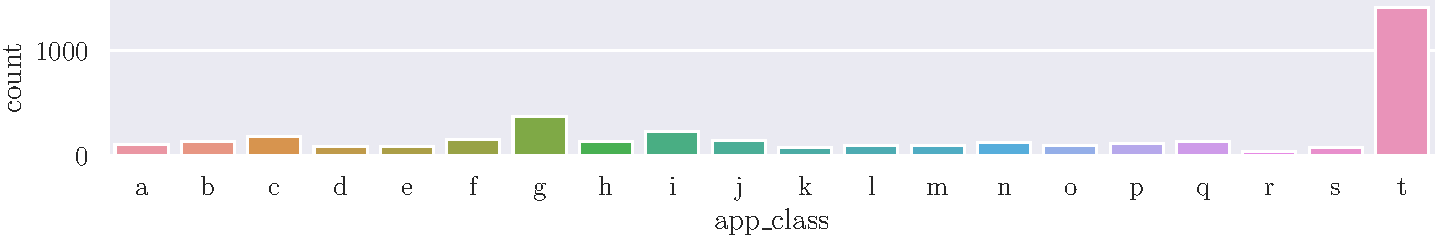
\includegraphics[width=.83\textwidth]{app_class_countplot_in_days}
    \caption{B中各类APP计数图}
    \label{fig:001}
\end{figure}

\subsection{数据探索之类别变量}

\subsubsection{单一变量}
\begin{table}[!htbp]
    \caption{类别变量统计描述(以day01为例)}\label{tab:002} \centering
    \begin{tabular}{llrll}
        \toprule[1.5pt]
               & $uid$                            & $appid$ & $app\_type$ & $app\_class$ \\
        \midrule[1pt]
        count  & 5335803                          & 5335803 & 5335803     & 5335803      \\
        unique & 35451                            & 11021   & 4           & 21           \\
        top    & A9E4AAC5B8E05D2A4E35E0D4F2994F37 & 3309    & usr         & NaN          \\
        freq   & 2629                             & 924309  & 2987468     & 2432606      \\
        \bottomrule[1.5pt]
    \end{tabular}
\end{table}

据\cref{tab:002}~,$app\_type$只有两类【系统预装、用户安装】,存在异常。通过数据探索,发现表格存在['sys', 'usr', '用户', '预装']四种取值,故将中文全部替换成英文。

$app\_class$有$21$类,这是因为在“左连接”操作时,将$NaN$也作为一种APP类型,这是由于此处数据缺失本身就代表一种资讯(小众APP),并非随机发生或人为故意。如果将$NaN$ 也视作一种$app\_class$,那么数据$B$ 不存在缺失值。

\subsubsection{天数变化}
另外,从21天的类型变量数据可以发现,每日活跃用户、APP、日志条数在各天都有所差异,如\cref{fig:002}~所示。

\begin{figure}[!htbp]
    \centering
    \begin{minipage}[c]{0.3\textwidth}
        \centering
        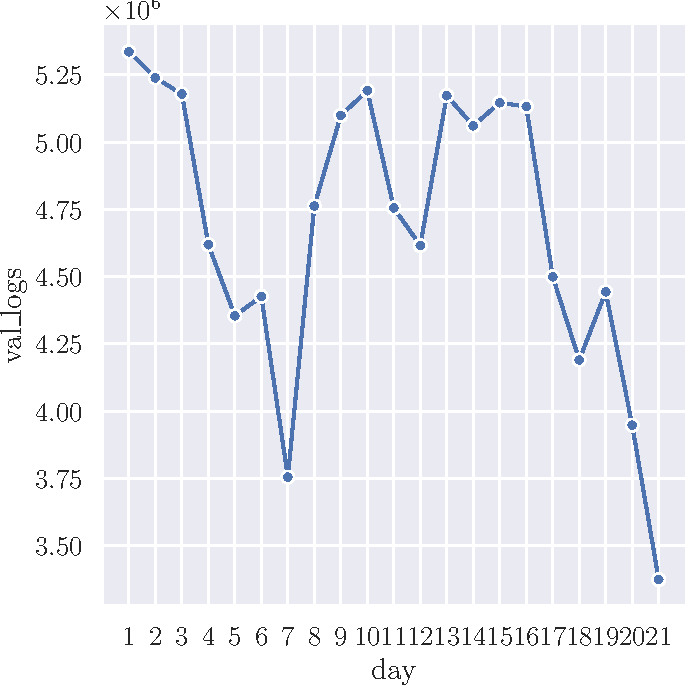
\includegraphics[width=0.95\textwidth]{relplot_line_day_val_logs}
        \subcaption{日志条数}
        \label{fig:002-a}
    \end{minipage}
    \begin{minipage}[c]{0.3\textwidth}
        \centering
        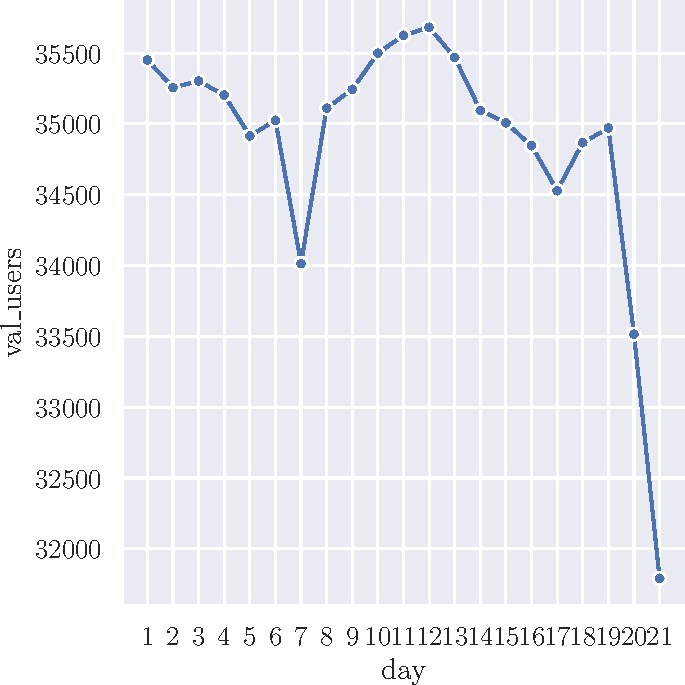
\includegraphics[width=0.95\textwidth]{relplot_line_day_val_users}
        \subcaption{活跃用户数}
        \label{fig:002-b}
    \end{minipage}
    \begin{minipage}[c]{0.3\textwidth}
        \centering
        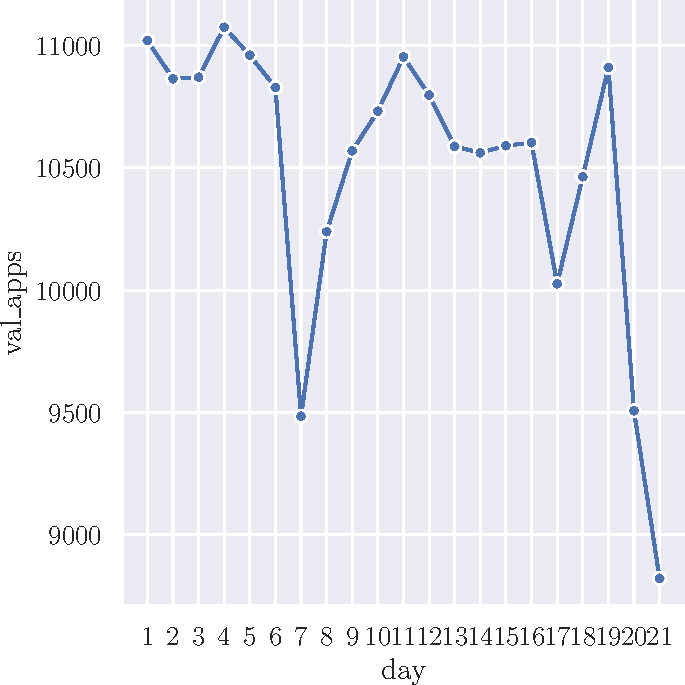
\includegraphics[width=0.95\textwidth]{relplot_line_day_val_apps}
        \subcaption{活跃APP数}
        \label{fig:002-c}
    \end{minipage}
    \caption{day01~day21类别变量的变化折线图}
    \label{fig:002}
\end{figure}

粗略观察\cref{fig:002-b},活跃用户数在$7$和$21$存在明显波谷,似乎和“星期”有某种关联;对照\cref{fig:002-a}、\cref{fig:002-b}、\cref{fig:002-c}三表分析,似乎APP活跃情况(种类、请求)与天数有所关联,甚至可以猜测某些小众APP被某些特定用户群体所使用甚至是青睐。

\subsubsection{变量关联}

APP自身包含$appid$、$app\_class$以及$app\_type$属性,因此可以抽取这三列建立$C$。

\begin{table}[!htbp]
    \caption{APP统计描述}\label{tab:003} \centering
    \begin{tabular}{lrll}
        \toprule
               & $appid$ & $app\_type$ & $app\_class$ \\
        \midrule
        count  & 37276   & 37276       & 37276        \\
        unique & 36437   & 2           & 21           \\
        top    & 19582   & usr         & NaN          \\
        freq   & 2       & 34153       & 32958        \\
        \bottomrule
    \end{tabular}
\end{table}

据\cref{tab:003}~,数据探索发现有839个app多重类型,即对于某些用户而言,该软件为系统预装,对另一些而言,则为自行安装。这似乎表明,不同的用户在软件下载与安装层面,有可相互区分的行为特征。另外,21类APP的数量情况如\cref{fig:003}~所示。

\begin{figure}[!htbp]
    \centering
    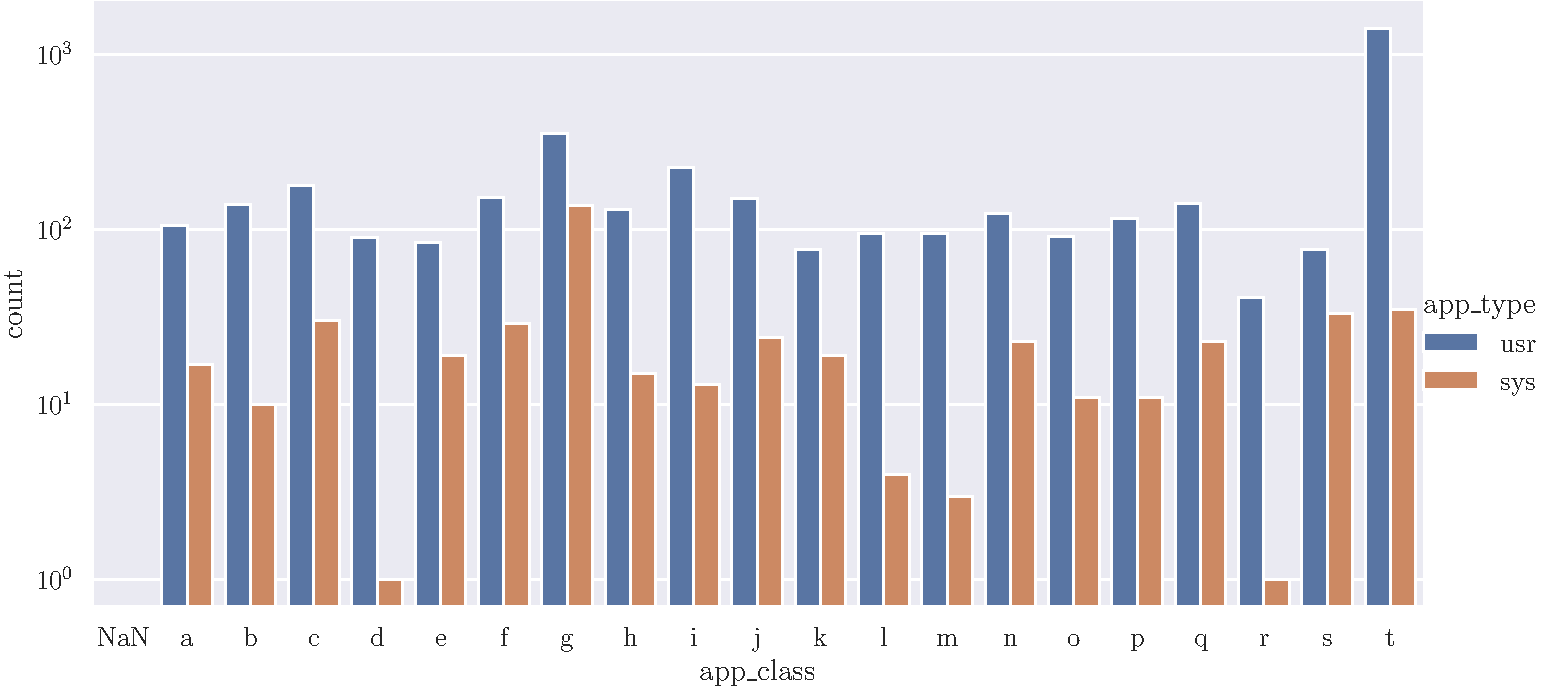
\includegraphics[width=.95\textwidth]{catplot_count_app_class}
    \caption{21类APP计数图}
    \label{fig:003}
\end{figure}

据\cref{fig:003}~,未分类的APP并不是小数目(有一部分为系统预装),$t$类在APP多样性表现上依然出众。此外,不同种类的APP就类型(预装、用户)而言相差较为悬殊,例如:$g$类,系统预装相对较多;其余类别,用户预装较为普遍,尤其是$d$和$r$类。

值得区分的是,在新建APP统计数据$C$中,计数图反映了各类APP的多样程度(市场垄断程度)。而在监测数据$B$中,某个(类)APP请求日志(行数)计数图则反映了该用户在使用各类APP时的活跃(点击)行为,这将在下一小节进行探索。

\subsection{数据探索之数值变量}

\subsubsection{单一变量}

\begin{table}[!htbp]
    \caption{数值变量统计描述(以day01为例)}\label{tab:004} \centering
    \begin{tabular}{lrrrrr}
        \toprule[1.5pt]
              & $start\_day$ & $end\_day$ & $duration$     & $up\_flow$      & $down\_flow$   \\
        \midrule[1pt]
        count & 5335803      & 5335803    & 5335803        & 5335803         & 5335803        \\
        mean  & 0.975107     & 1          & 2151.604772    & 607572.168995   & 158163.759549  \\
        std   & 16.843899    & 0          & 1455335.155631 & 11015502.975274 & 6538529.614936 \\
        min   & -16524       & 1          & 1              & 0               & 0              \\
        25\%  & 1            & 1          & 3              & 0               & 0              \\
        50\%  & 1            & 1          & 10             & 0               & 0              \\
        75\%  & 1            & 1          & 36             & 1278            & 1063           \\
        max   & 1            & 1          & 1427769883     & 3639473769      & 3292713011     \\
        \bottomrule[1.5pt]
    \end{tabular}
\end{table}

数据具体说明指出:“$start\_day$:使用起始天,取值1-30(注:第一天数据的头两行的使用起始天取值为0,说明是在这一天的前一天开始使用的)。”然而,\cref{tab:004}~显示其最小值为$-16542$,因此可以判断$start\_day$存在异常值;而这会直接导致$duration$、$up\_flow$、$down\_flow$偏差过大。因此,须要对这两列进行数据清洗,删除异常值。

\begin{figure}[!htbp]
    \centering
    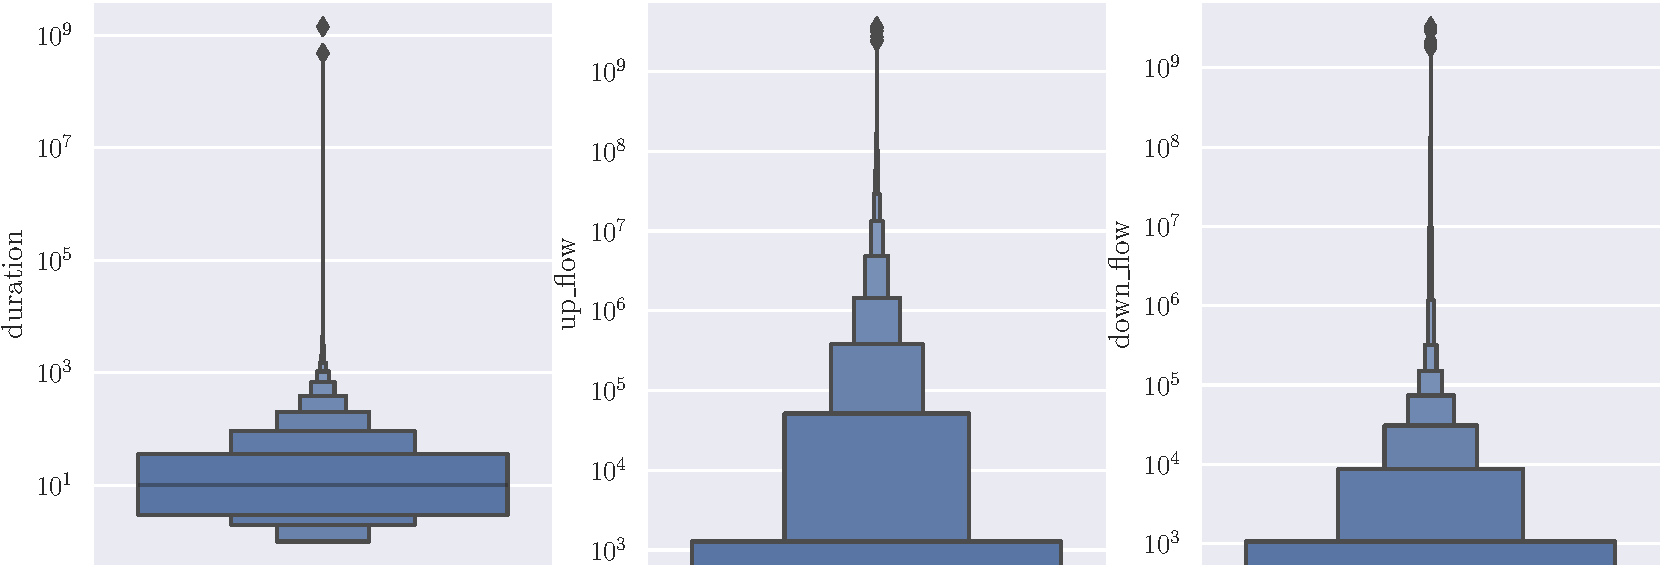
\includegraphics[width=.95\textwidth]{boxenplot_duration_day01}
    \caption{使用时长、上下行流量增强箱形图(以day01为例)}
    \label{fig:004}
\end{figure}

据统计,在第1~21天监测数据中,$99.98\%$的记录使用时长不超过$9158.02$。针对异常案例进行分析,例如,$uid=64B3E40461C56847F35DB46D55707EA4$用户:

\begin{table}[!htbp]
    \caption{异常案例}\label{tab:005} \centering
    \begin{tabular}{lllllrlrlrrr}
        \toprule[1.5pt]
        appid & app\_class & start\_day & start\_time & end\_day & end\_time & duration \\
        \midrule[1pt]
        4803  & a          & 19         & 00:52:46    & 19       & 07:47:59  & 24912    \\
        18478 & c          & 19         & 07:48:25    & 19       & 07:48:38  & 12       \\
        \.    & \.         & \.         & \.          & \.       & \.        & \.       \\
        6192  & NaN        & 19         & 20:46:11    & 19       & 20:46:29  & 18       \\
        3309  & f          & 19         & 23:14:49    & 19       & 23:16:38  & 109      \\
        \bottomrule[1.5pt]
    \end{tabular}
\end{table}

凌晨零时至早上七时的记录是不符合生活常态不可持续的,猜测是应用后台驻留、系统故障或用户因故未关闭应用。不过,是否存在异常行为可以作为一个新的特征。因此,本文对持续时间超过$9159$的认定为无效使用时长,不能真实反映用户的行为特征。

此外,以第一天为例,不同用户在$appid$个数、$duration$总时长、$up\_flow$、$down\_flow$总流量、日志行数层面有所差异,分布如\cref{fig:005}~所示。

\begin{figure}[!htbp]
    \centering
    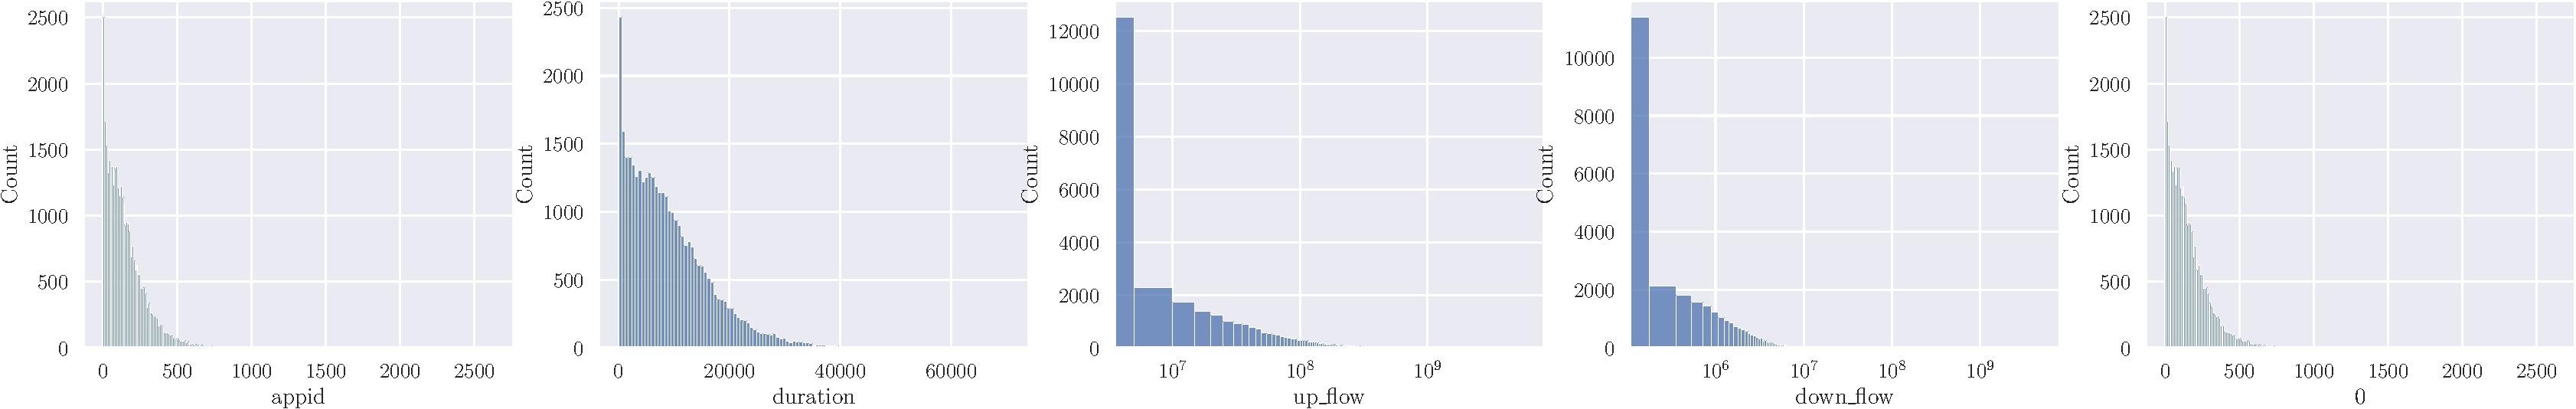
\includegraphics[width=.95\textwidth]{histplots_appid_duration_upflow_downflow_lines}
    \caption{直方图(使用APP数量、使用有效总时长、消耗上下行流量、日志行数)}
    \label{fig:005}
\end{figure}

可以观察到某些用户较依赖手机,日志数、使用时长、APP多样性、消耗流量偏多。

\subsubsection{天数变化}

探索发现,可为每名用户绘制使用APP总数/时长/流量/日志随天数变化的折线图,以展现用户在月(周)级别的变化趋势与独潜在规律,并据此将用户群归类。

\subsubsection{变量关联}

更细粒度地,对于每名用户/每天,可绘制其各类APP的个数/时长/流量/日志情况,以了解用户对不同类型APP的适用情况、青睐程度;更进一步,还可以绘制24小时各类APP使用情况,这样便于了解用户的作息、通勤、活跃时段等信息。

\subsection{直觉小结与用户量化}

\subsubsection{数据直觉}
概括来说,赛题数据$A$给出4000多个常用APP所属类别:这是$1:1$的数据;而赛题数据$B$则记录了每名用户($uid$)每日每时使用各款APP($appid$)的起始时间,使用时长,上下流量等信息:这是$1:N$的资料。可以使用统计量进行归纳。

具体而言,监测数据蕴藏大量用户行为特征,例如:
\begin{itemize}
    \item 用户一天使用多长时间的手机(可间接反映依赖程度、年龄)
    \item 用户平均多长时间看一次手机(可间接反映依赖程度、年龄、工作)
    \item 距离上一次上线,隔了几天(可间接反映依赖程度、年龄、工作)
    \item 在什么星期几的时间段最常用什么类型APP(可反映工作、生活)
    \item 用户早、晚各使用什么类APP(可反映工作、生活、作息)
    \item 用户周末、工作日各使用什么类APP(可反映工作、生活、作息)
    \item 用户最早什么时候开始使用手机、什么时候结束使用(可反映工作、作息)
    \item 用户最常用什么类型APP(可反映喜好)
    \item 哪一类APP使用最频繁、哪一类使用时长最多(可反映喜好)
    \item 用户一共安装了多少个APP(可反映保守程度、对多样性的接纳程度)
    \item 系统预装与自行安装的比例(可反映保守程度、对多样性的接纳程度)
    \item 用户的每月流量使用情况(可间接反映财富程度、年龄)
\end{itemize}

\subsubsection{用户模型}

用户量化是指将现实生活中的“用户实体”进行抽象,采用不同维度的量化指标建模,即将其视为$n$维空间的一个点,使用形如$X=[x_1, x_2, \cdots , x_n]$的数学符号表示。

基于对数据集的深入探索及理解,提出简易用户模型:

\begin{table}[!htbp]
    \caption{简易用户模型}\label{tab:006} \centering
    \begin{tabular}{lllllrlrlrrr}
        \toprule[1.5pt]
        符号             & 意义                               & 维度                   \\
        \midrule[1pt]
        $uid$          & 用户的唯一标识                          & $1$                  \\
        $DU_{d, h, c}$ & 该用户在第$d$天$h$时内使用$c$类APP时,投入的总计时长 & $d\times h \times c$ \\
        $UF_{d, h, c}$ & 该用户在第$d$天$h$时内使用$c$类APP时,消耗的上行流量 & $d\times h \times c$ \\
        $DF_{d, h, c}$ & 该用户在第$d$天$h$时内使用$c$类APP时,消耗的下行流量 & $d\times h \times c$ \\
        $NO_{d, h, c}$ & 该用户在第$d$天$h$时内使用$c$类APP时,记录的日志行数 & $d\times h \times c$ \\
        \bottomrule[1.5pt]
    \end{tabular}
\end{table}

\section{问题一:聚类分析与用户画像}

\subsection{特征工程与评价指标}

\subsubsection{特征选择与数据降维}

聚类指将数据样本对象划分成若干类(簇、标签)并尽可能的保证“类内紧凑”、“类间独立”\cite{数据仓库与数据挖掘}。不同的量化指标、不同的相似度量(距离定义),往往会带来迥异的聚类结果。一般来说,量化指标维度数目越多,算法运行时间越长、结论可解释性越弱。

关于用户画像的量化指标,陈\cite{陈纯}、成\cite{成雪}等人从\uwave{日均屏幕使用时间}切入;
武\cite{武慧娟}等人从\uwave{APP数量、阅读时间}等特征对阅读类APP使用人群进行聚类解读;
侯\cite{侯金凤}针对\uwave{每日手机使用时长}、\uwave{使用频次}、\uwave{使用偏好}等特征对用户进行建模;
韦\cite{韦磊}基于\uwave{安装数量}、\uwave{打开次数}、\uwave{使用时长}、\uwave{工作日使用时长}、\uwave{周末使用时长}构建用户特征。

首先,为避免数据泄漏,仅选择前7日各类APP总时长、频次、上下行流量作为量化特征,共计$20 \times 4=80$维;对于不同的量纲特征,分别扣除均值,除以标准差以进行数值标准化。Pearson相关热力\cref{fig:pearson}~显示,各类APP时长、频次、流量成弱正相关。

\begin{figure}[!htbp]
    \centering
    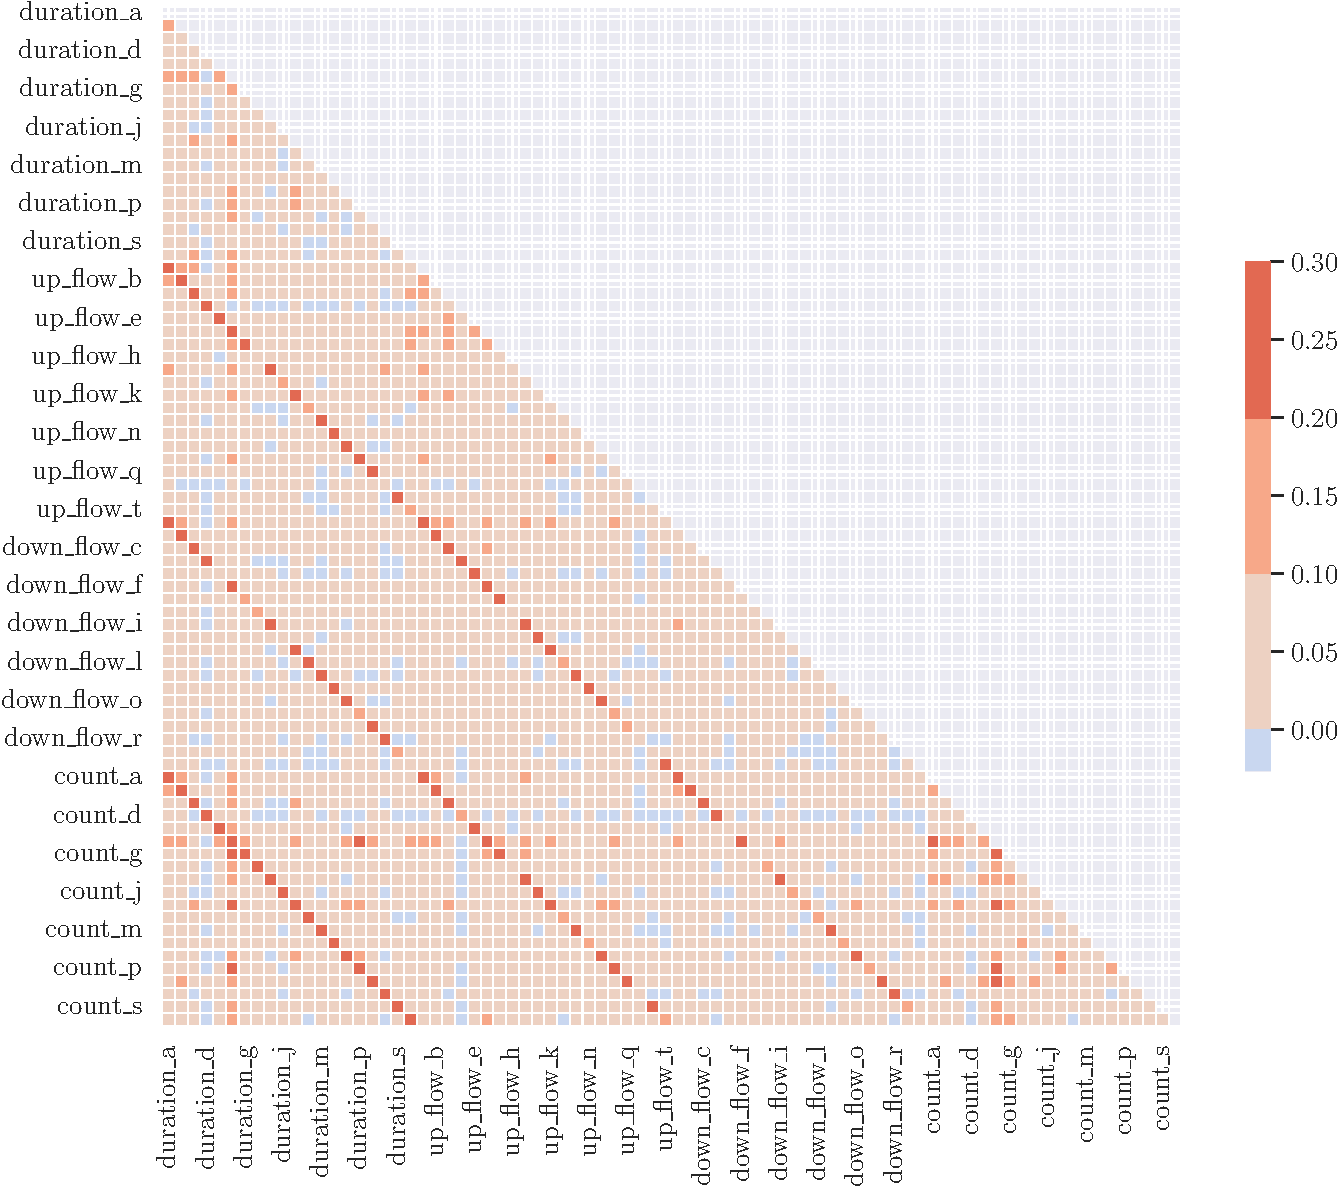
\includegraphics[width=.91\textwidth]{heatmap_features}
    \caption{皮尔逊相关系数热力图}
    \label{fig:pearson}
\end{figure}

为增加数据易用性,降低计算开销,增强视觉理解,而后采用主成分分析对特征进行变换,并按方差排序表示各维度重要程度,如\cref{fig:bar-pca}~,选定阈值将维度压缩至$3$维。

\begin{figure}[!htbp]
    \centering
    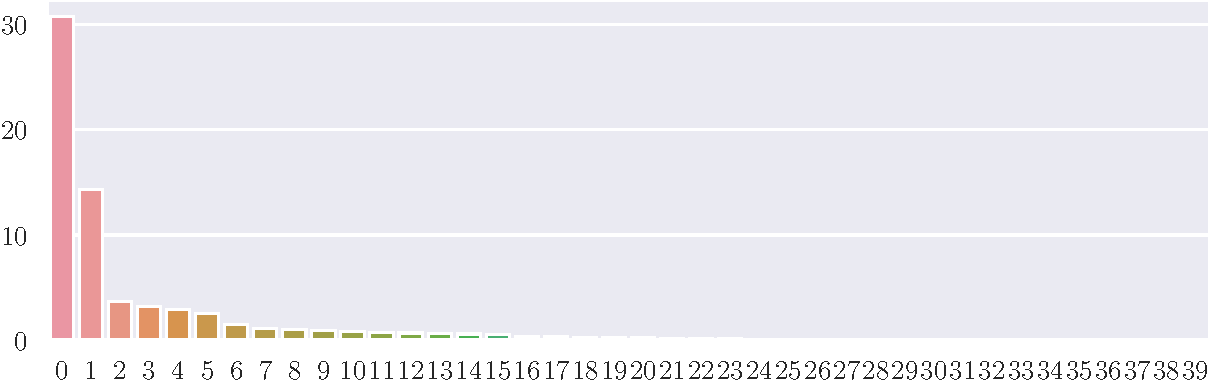
\includegraphics[width=.91\textwidth]{barplot_pca_features}
    \caption{PCA特征方差柱状图}
    \label{fig:bar-pca}
\end{figure}

\subsubsection{评价指标}

聚类“好坏”不存在绝对的客观的标准\cite{机器学习};聚类数目设定是否“合理”也往往依赖人工先验知识\cite{高维数据的聚类分析}。聚类数目设定过低,划分粒度不够细腻;聚类数目设定过高,宏观结论的可解释性又受到限制。常用选择聚类数目方法是人为观察聚合系数折线图,大致估计最优聚类数量$K$。相关定义如下:

\begin{definition}
    \textbf{各簇畸变程度}:该簇重心与其内部成员位置距离的平方和;
    假设一共将$n$个样本划分到$K$个簇中,用$C_k$表示第$k$簇,该簇重心记为$u_k$,则第$k$簇的畸变程度为:
    \begin{equation}
        \sum_{i\in C_k} |x_i-u_k|^2
        \label{eq:001}
    \end{equation}
    \label{def:001}
\end{definition}

\begin{definition}
    \textbf{聚合系数}:
    \begin{equation}
        J=\sum_{k=1}^{K} \sum_{i \in C_k} |x_i-u_k|^2
        \label{eq:002}
    \end{equation}
    \label{def:002}
\end{definition}

此外,还有Calinski-Harabasz系数\cite{CH}、Davies-Bouldin指数\cite{DB}、Silhouette轮廓系数\cite{SC}可用于度量某些聚类目的下的结论性能。

\subsection{算法概述与K值选择}

注:本小节所使用算法及评价指标均采用scikit\_learn\cite{sklearn}实现。

\subsubsection{原型聚类:K-Means++}

K-Means是一种简单、高效的聚类算法,假设聚类结构能通过一组“原型”刻画,算法的主要思想是通过迭代过程把数据集划分为不同的类别,流程如\cref{fig:008}~。K-means++优化“初始化K个聚类中心”,要求初始的聚类中心之间的相互距离要尽可能的远,在“孤立点数据敏感性”方面优于K-Means算法。默认采用欧式距离、重心法进行相似度量。

\begin{figure}[!htbp]
    \centering
    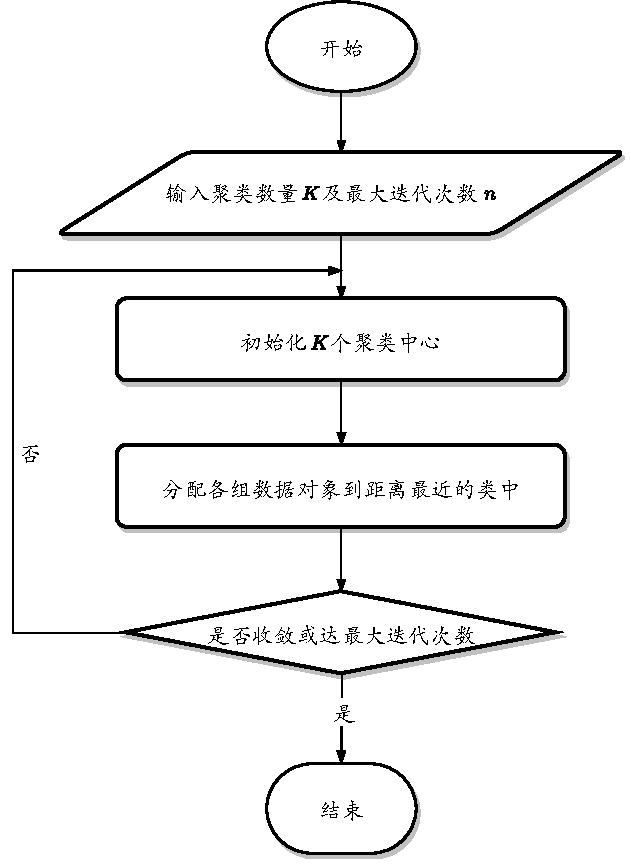
\includegraphics[width=.37\textwidth]{process_kmeans}
    \caption{KMeans算法流程图}
    \label{fig:008}
\end{figure}

将最大迭代次数设置为1000,选择K等于2~50绘制聚合系数与卡林斯基-哈拉巴斯指数折线图。根据\cref{fig:009}~,K值从2到13时,畸变程度变化最大;超过6畸变程度变化显著降低:因此根据肘部法则,可将聚类数量$K$设定为5;从来看,应将聚类数量设定为6以下。该结论符合卡林斯基-哈拉巴斯指数峰值,故将聚合数目设定为$5$。

\begin{figure}[!htbp]
    \centering
    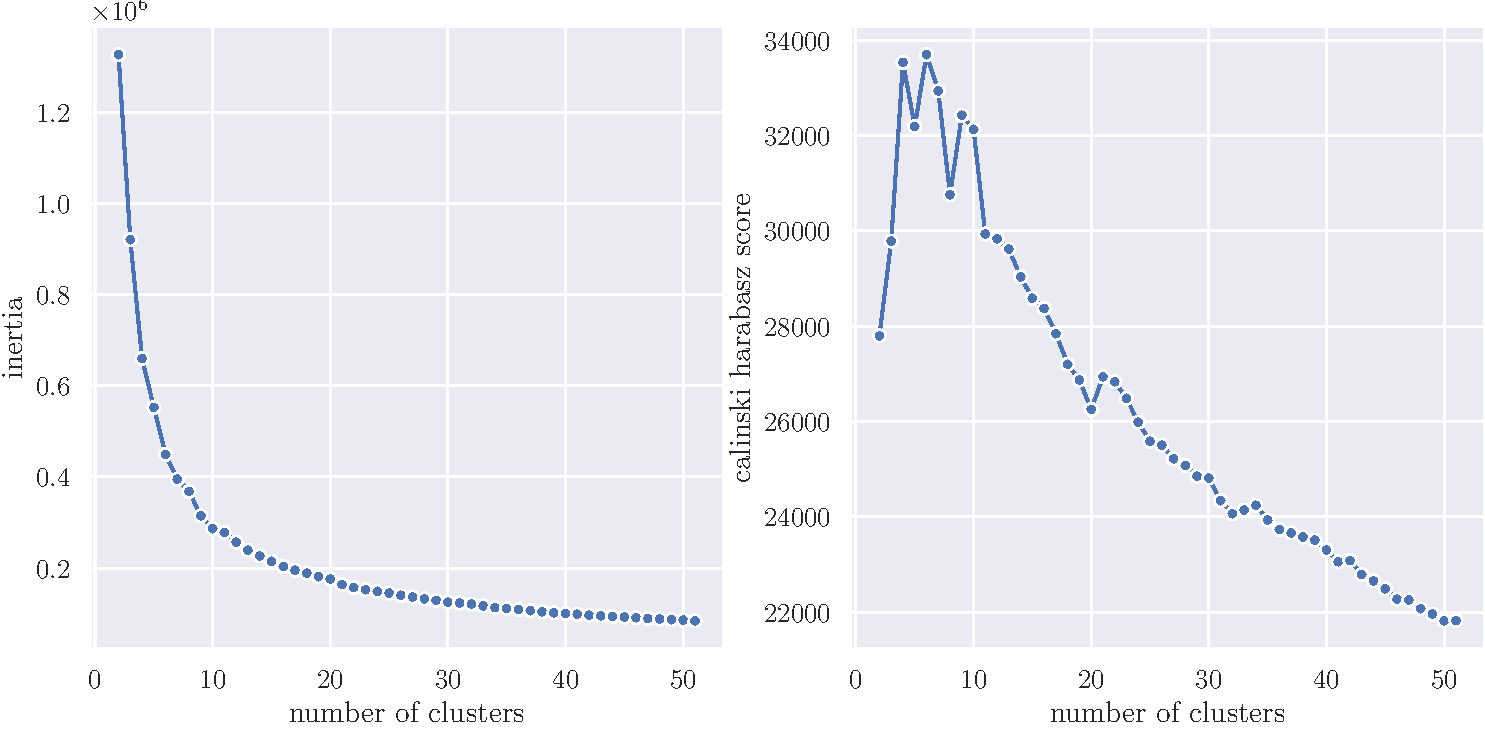
\includegraphics[width=.77\textwidth]{lineplot_Ks_inertias_CH.pdf}
    \caption{K-Means 聚合系数与卡林斯基-哈拉巴斯指数}
    \label{fig:009}
\end{figure}

\subsubsection{层次聚类:BIRCH+AGNES}

AGNES算法(Agglomerative
Nesting),以自底向上方式,不断重复合并,产生不同粒度(层次)的聚类结果,一般最终预设聚类数目为1。该算法默认采用“欧式距离”进行度量样本距离,采用“离差平方和”(ward
linkage)作为簇距离度量函数,可通过聚类谱系图(dendrogram)可视化,算法执行流程如下:

\IncMargin{1em}
\begin{algorithm} \SetKwData{Left}{left}\SetKwData{This}{this}\SetKwData{Up}{up} \SetKwFunction{Union}{Union}\SetKwFunction{FindCompress}{FindCompress} \SetKwInOut{Input}{input}\SetKwInOut{Output}{output}

    \Input{样本集$D=\{ x_1, x_2, \ldots, x_m \}$; \\
        聚类簇距离度量函数$d$;\\
        聚类簇数$k$。}
    \Output{簇划分:$\mathcal{C}=\{ C_1, C_2, \ldots, C_k \}$ }
    \BlankLine

    \BlankLine
    \emph{\#先将每个样本视作一个初始簇构造}\;
    \emph{\#构造$M$个类,每个类仅包含一个样本}\;
    \For{$j = 1,2, \ldots, m$}{
    $C_j={x_j}$
    }

    \BlankLine
    \emph{\#两两计算距离}\;
    \For{$i = 1,2, \ldots, m$}{
    \For{$j = i+1, \ldots, m$}{
    $M_{i, j}=d(C_i, C_j)$\;
    $M_{j, i}=M_{i, j}$
    }
    }

    \BlankLine
    \emph{\#当前类个数大于预设簇数}\;
    \While{$q > k$}{

    合并距离最近的两个聚类簇$C_{i^*}= C_{i^*} \cup C_{j^*}$\;
    \For{$j=j^*+1, j=j^*+2, \ldots, q$}{
        将聚类簇$C_{j}$重编号为$C_{j-1}$
    }

    删除距离矩阵$M$的第$j*$行与第$j*$列\;
    \# 重新计算距离矩阵\;
    \For{$j=1,2, \ldots, q-1$}{
    $M_{i^*, j}=d(C_{i^*}, C_{j})$\;
    $M_{j, i^*}=M_{i^*, j}$
    }
    q=q-1
    }
    \caption{AGNES算法}
\end{algorithm}
\DecMargin{1em}

AGNES算法时间复杂度为立方级别,对于本题万级别用户而言,耗费时间过长。因此,本文首先采用BIRCH\cite{birch}聚类算法得到初步聚类质心,作为AGNES算法的输入。BIRCH算法综合了层次凝聚和迭代的重定位方法首先用自底向上的层次算法,然后用迭代的重定位来改进结果。它的主要思想是:扫描数据库,建立一个初始存放于内存中的聚类
特征树然后对聚类特征树的叶结点进行聚类\cite{birch2}。

针对本题,首先将前7日44253名用户采用BIRCH算法聚类获得2827枚质心,而后AGNES对质心进行聚类,并绘制6层谱系图如下。

\begin{figure}[!htbp]
    \centering
    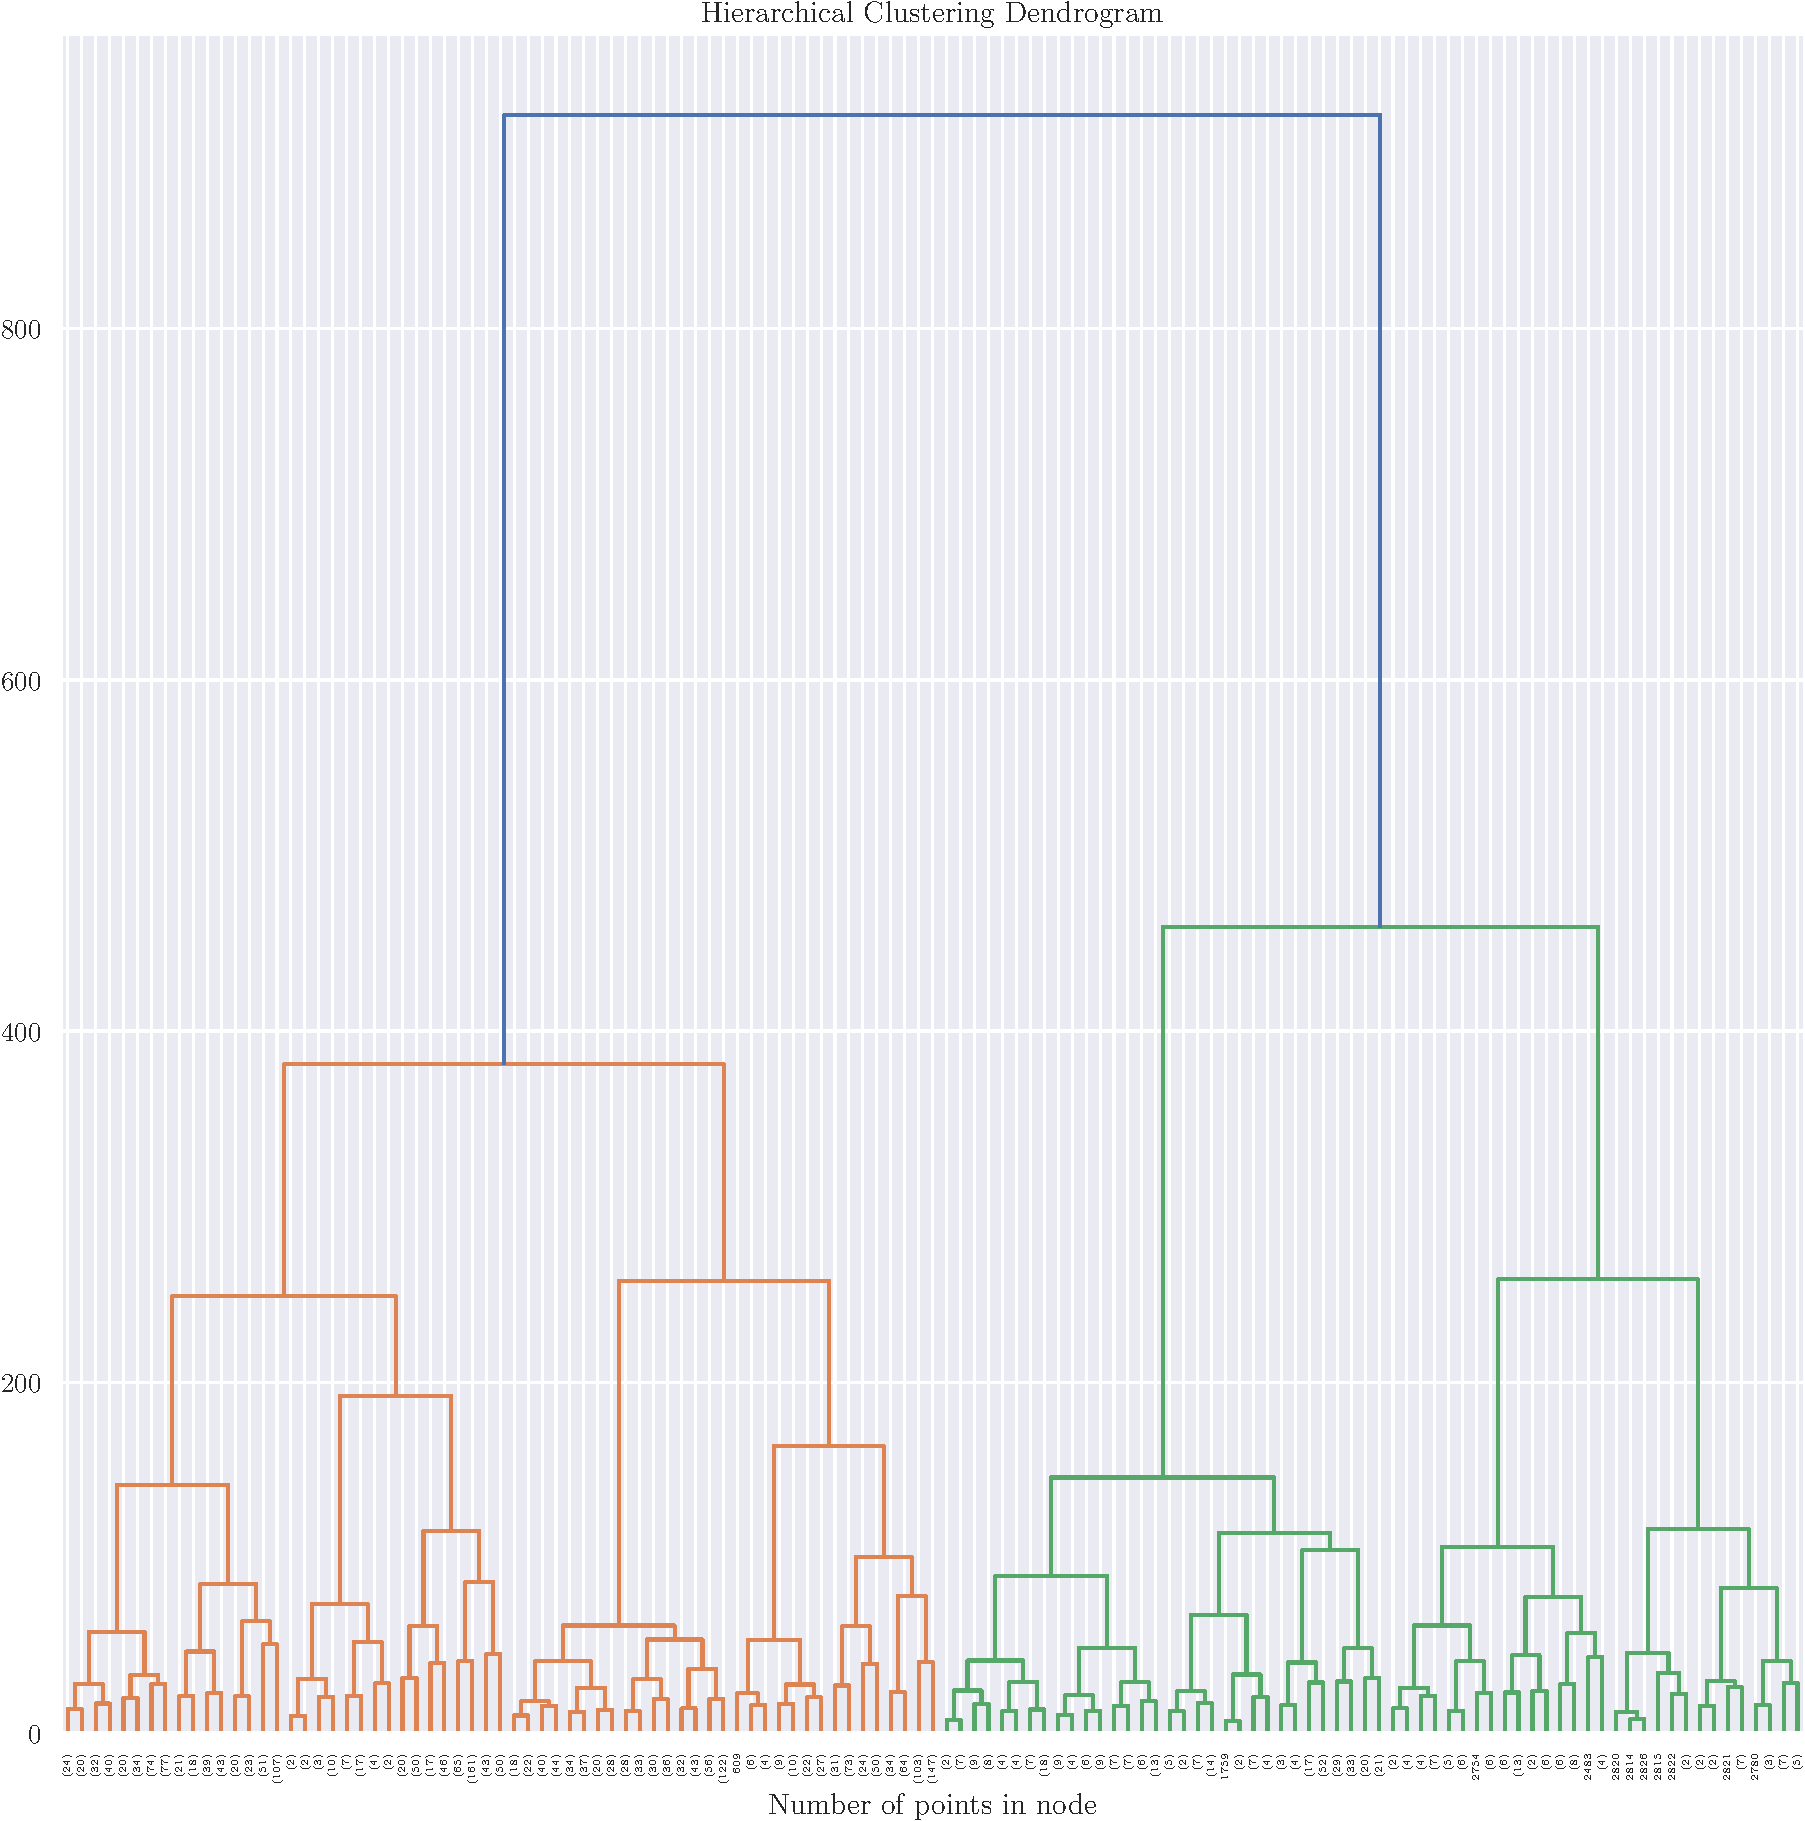
\includegraphics[width=.6\textwidth]{dendrogram}
    \caption{BIRCH+AGNES谱系图}
    \label{fig:010}
\end{figure}

\subsubsection{密度聚类:DBSCAN}

DBSCAN算法从样本密度的角度来考察样本之间的可连接性,要求聚类空间中的以$eps$为半径的邻域内所包含对象的数目不小于某一给定阈值$min\_samples$,并基于可连接样本不断扩展生长聚类簇以获得最终的聚类结果\cite{机器学习}。算法将数据样本点分为三类:

\begin{enumerate}
    \item 核心点:在半径$eps$内含有不少于$min\_samples$数目的点
    \item 边界点:在半径$eps$内点的数量小于$min\_samples$,但是落在核心点的邻域内
    \item 噪声点:既不是核心点也不是边界点的点
\end{enumerate}

DBSCAN不需要预先输入要划分的聚类个数,但是对$eps$、$min\_samples$参数敏感。记特征维度数目$N=3$、$K=2N-1$,按照以下经验值确定超参数\cite{eps1,eps2}:$min\_samples=2N=6$,将数据集各点与K-最近邻算法分类标签的距离排序,观察\cref{fig:011}~拐点$y$坐标确定$eps=2$。

运行结果如下,聚类数量为$7$,噪点用户$539$名。

\begin{figure}[!htbp]
    \centering
    \begin{minipage}[c]{0.49\textwidth}
        \centering
        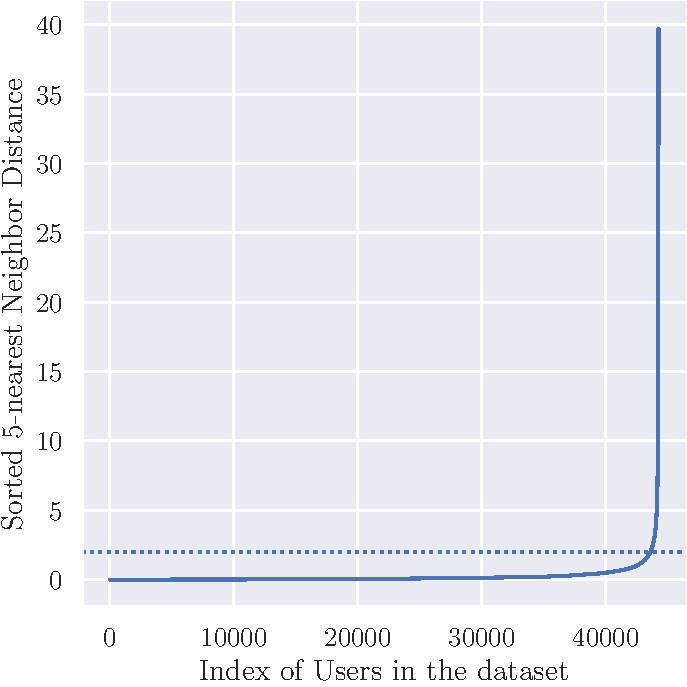
\includegraphics[width=.62\textwidth]{relplot_knn_distances}
        \caption{数据集各点6-最近邻距离(排序)}
        \label{fig:011}
    \end{minipage}
    \begin{minipage}[c]{0.49\textwidth}
        \centering
        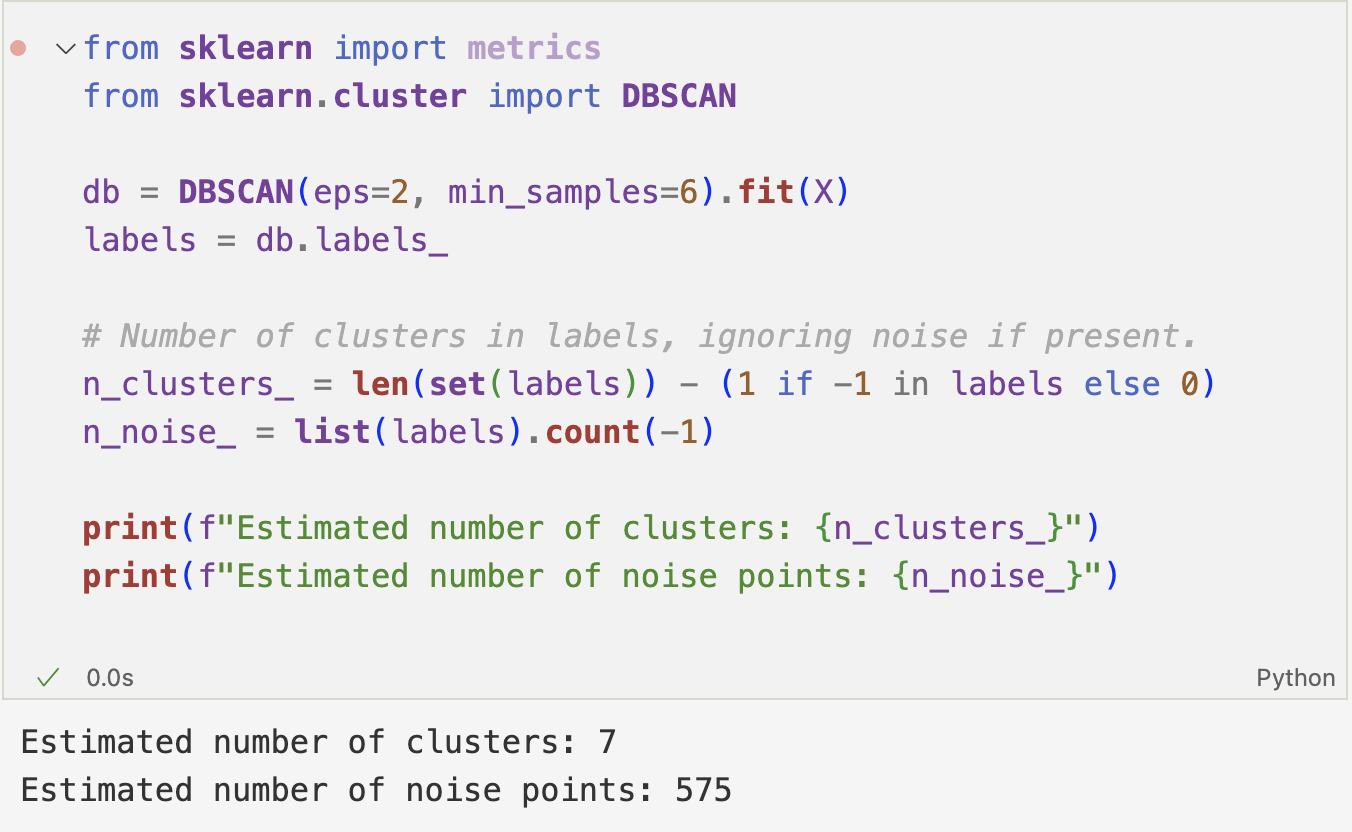
\includegraphics[width=.99\textwidth]{dbscan}
        \caption{Visual Studio运行结果截图}
        \label{fig:012}
    \end{minipage}
\end{figure}

\subsection{算法比较与用户画像}

\subsubsection{算法比较}

截取BIRCH+AGNES聚类数目为$6$时的聚类结果。先采用内部评价指标比较,再使用PCA降维特征绘制三维散点图,最后使用二维t-SNE\cite{tsne}可视化原始80维特征。

\begin{table}[!htbp]
    \caption{聚类算法内部评价指标}\label{tab:007} \centering
    \begin{tabular}{llrrr}
        \toprule[1.5pt]
          & $Method$    & $Calinski-Harabasz$            & $Davies-Bouldin$           & $Silhouette$               \\
        \midrule[1pt]
        0 & K-Means++   & \textit{\textbf{32187.076682}} & \textit{\textbf{0.766536}} & 0.511919                   \\
        1 & DBSCAN      & 2870.580217                    & 2.817892                   & \textit{\textbf{0.664019}} \\
        2 & BIRCH+AGNES & 24732.933816                   & 0.860360                   & 0.622801                   \\
        \bottomrule[1.5pt]
    \end{tabular}
\end{table}

\begin{figure}[!htbp]
    \centering
    \begin{minipage}[c]{0.25\textwidth}
        \centering
        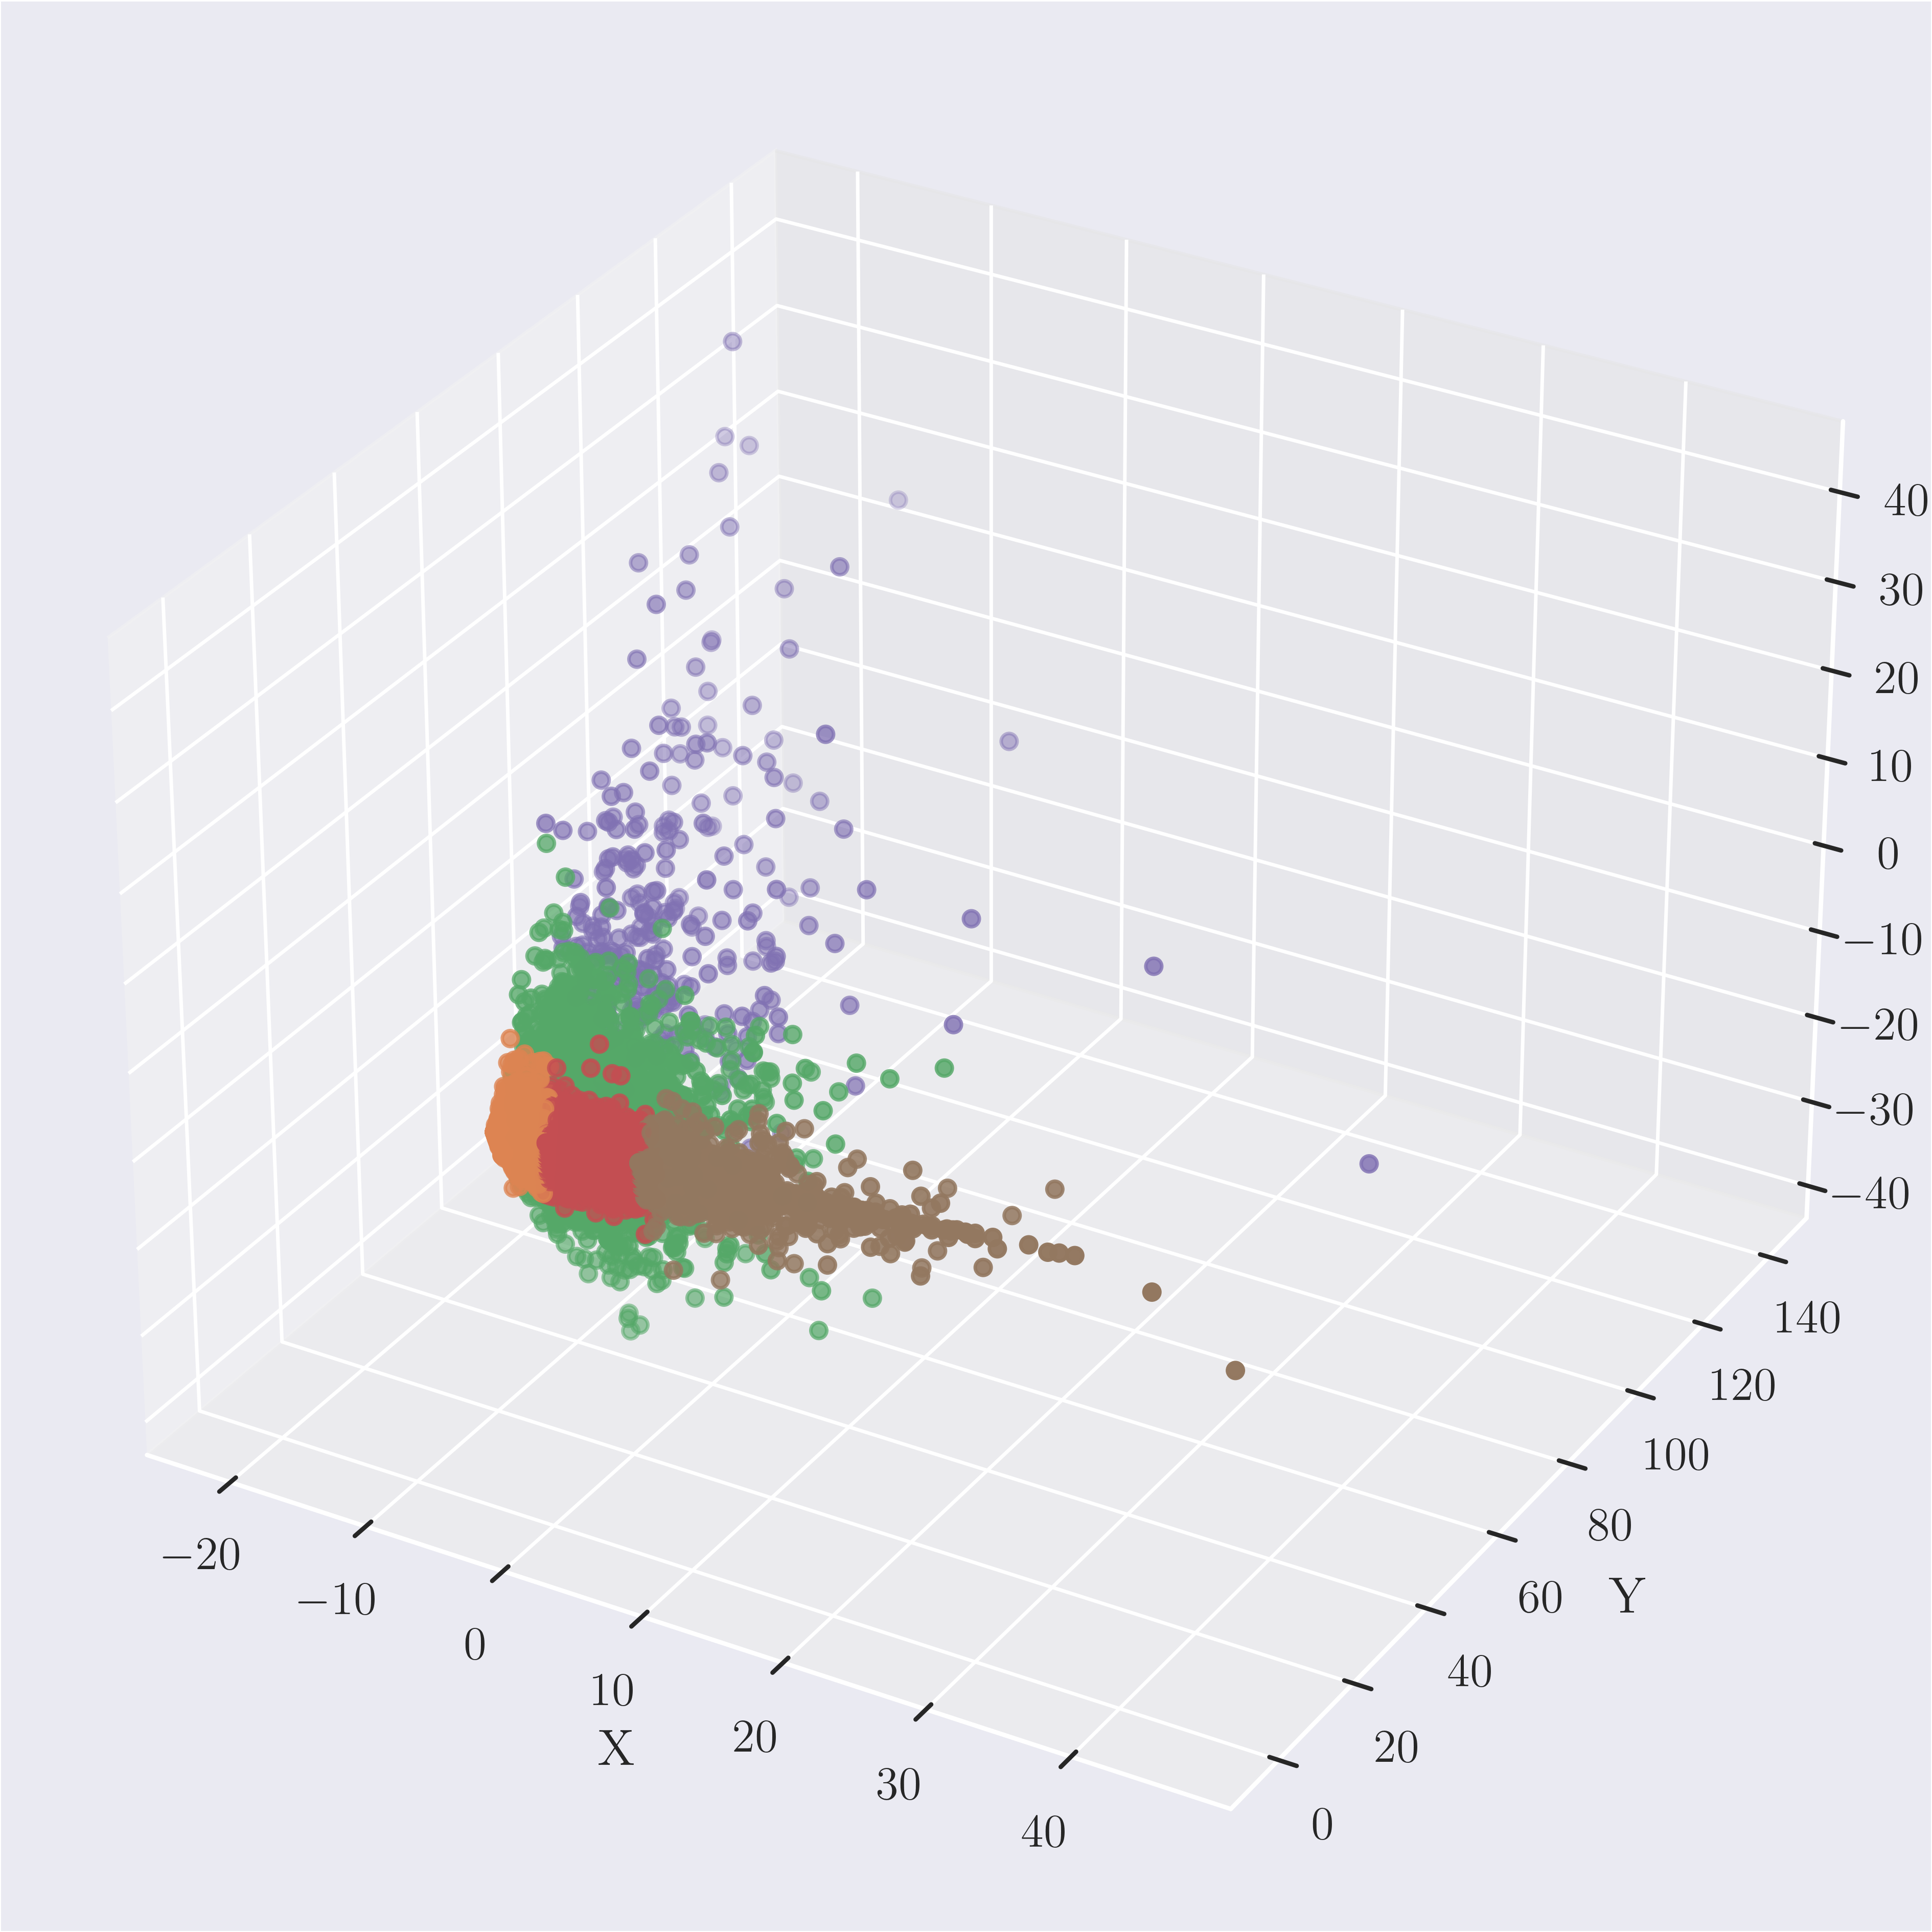
\includegraphics[width=0.99\textwidth]{3d_kmeans}
        \subcaption{K-Means++}
        \label{fig:013-a}
    \end{minipage}
    \begin{minipage}[c]{0.25\textwidth}
        \centering
        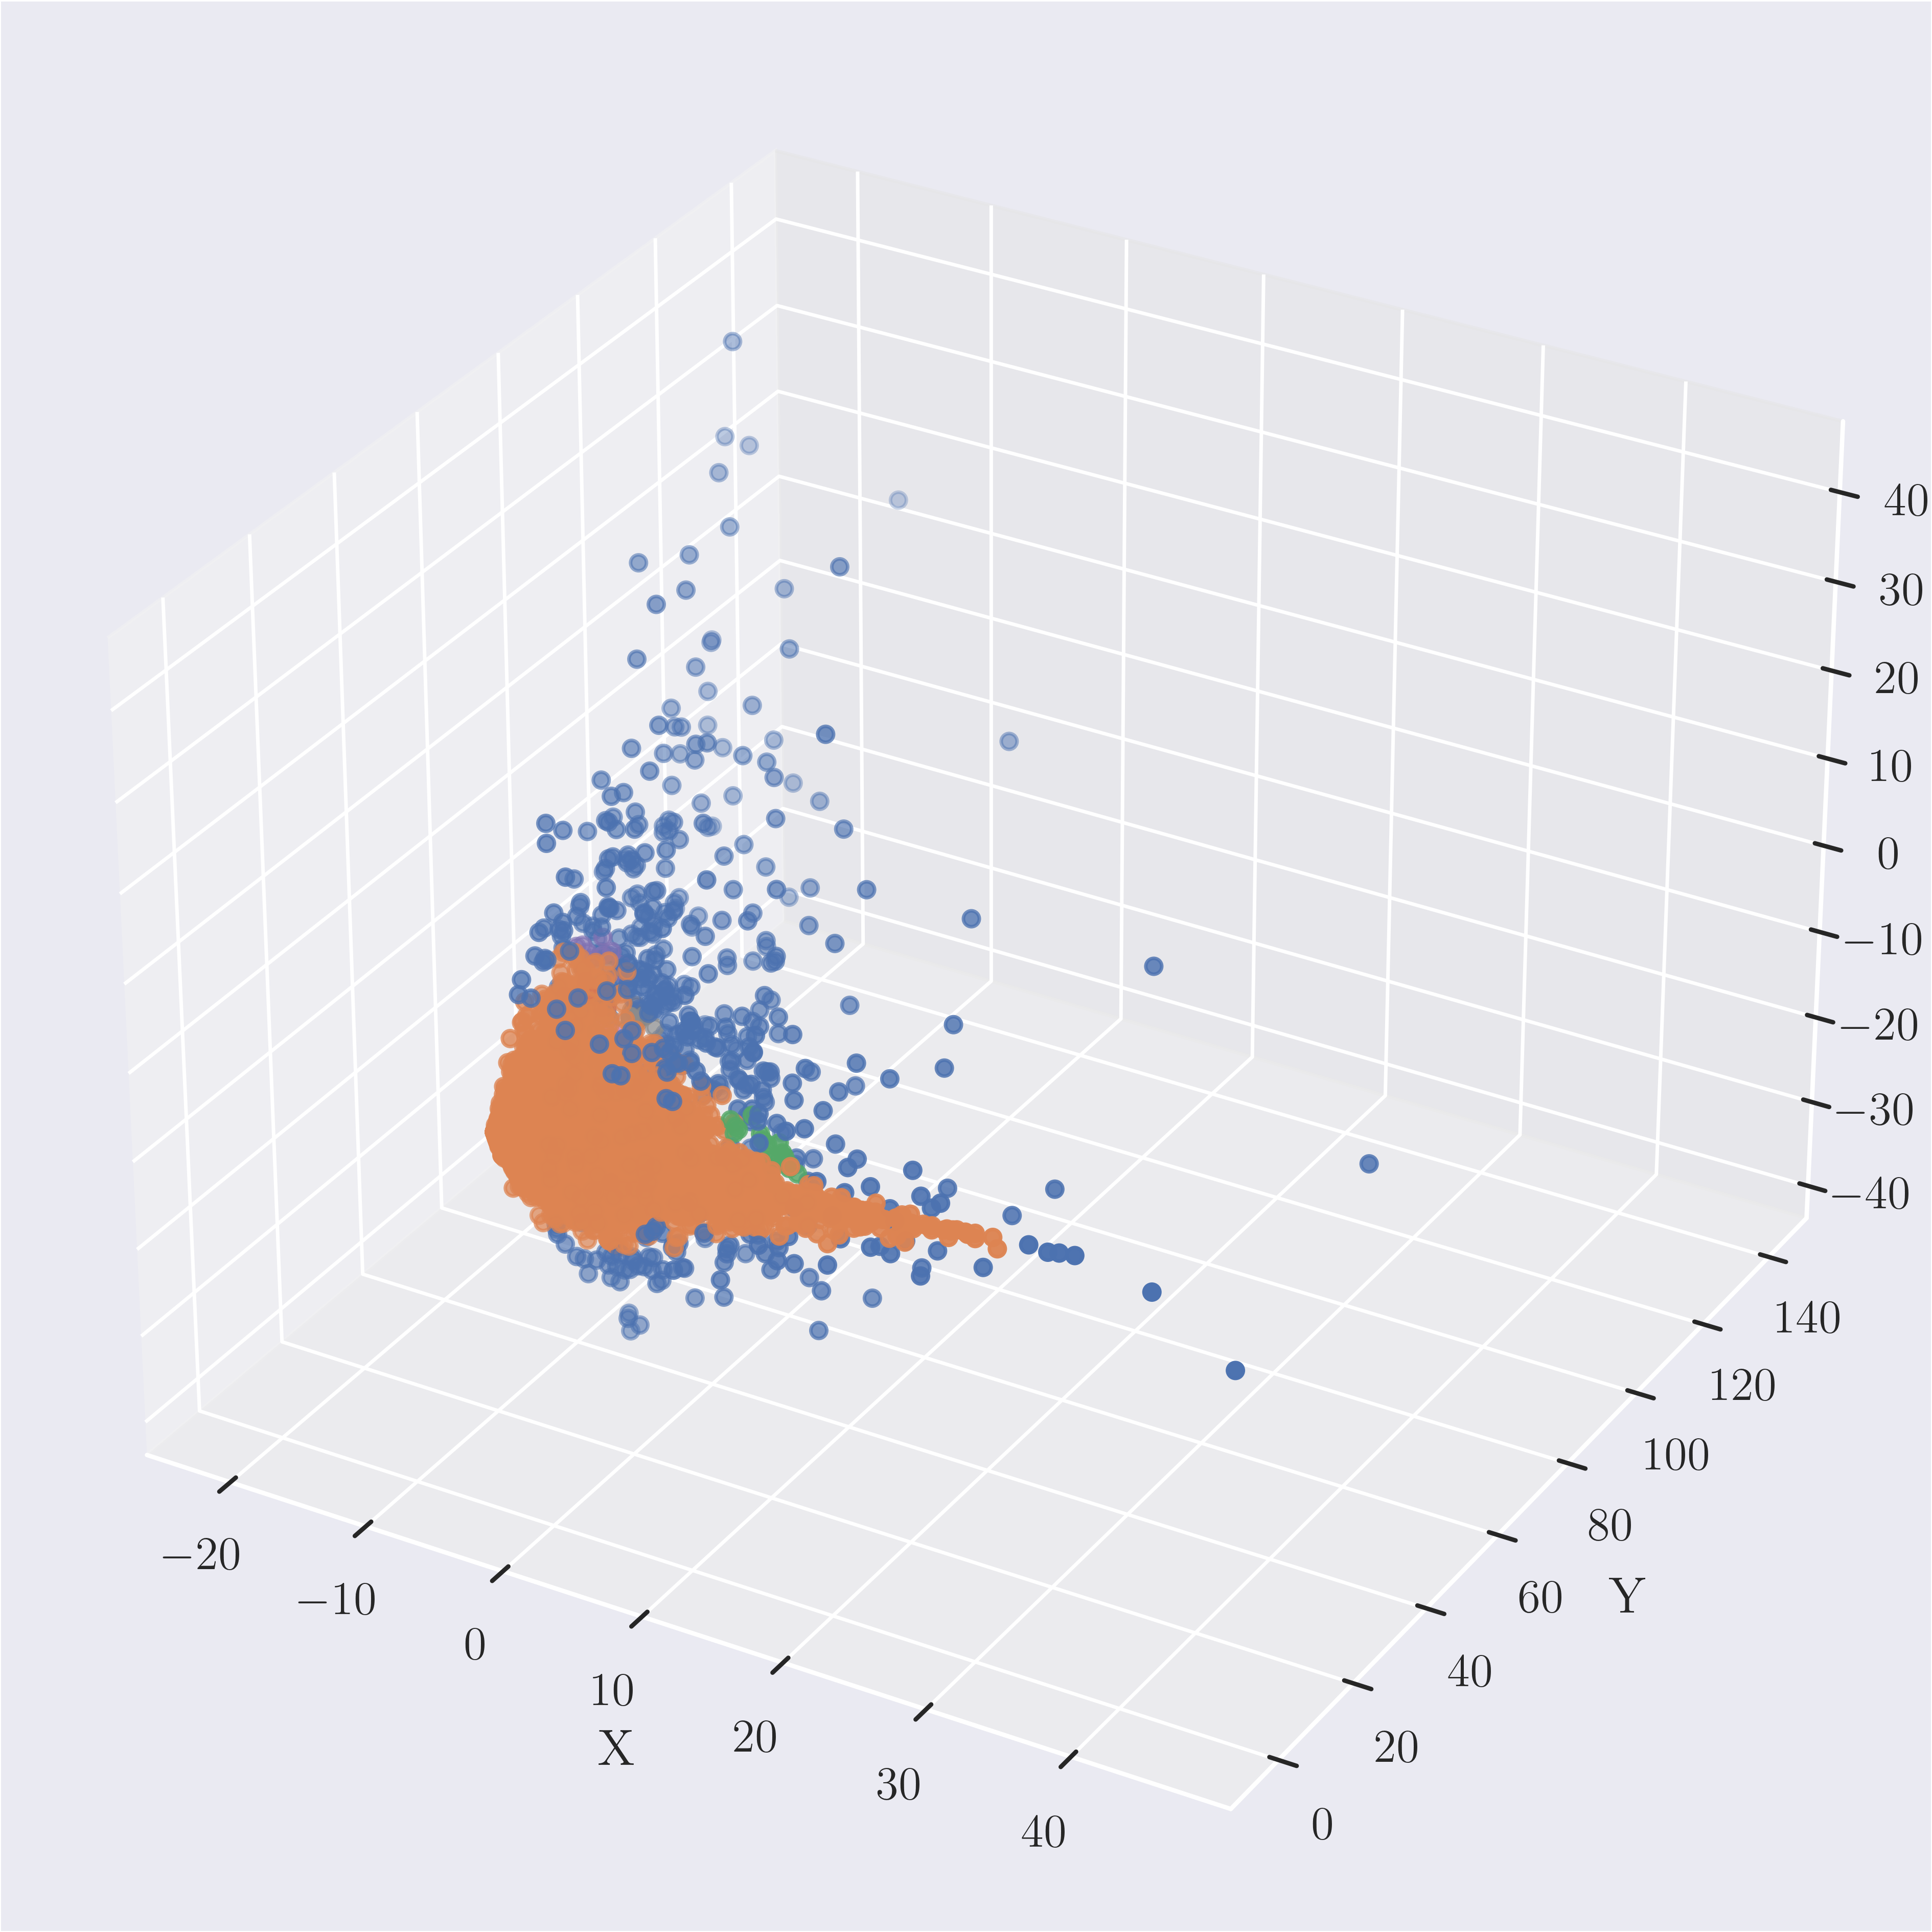
\includegraphics[width=0.99\textwidth]{3d_dbscan}
        \subcaption{DBSCAN}
        \label{fig:013-b}
    \end{minipage}
    \begin{minipage}[c]{0.25\textwidth}
        \centering
        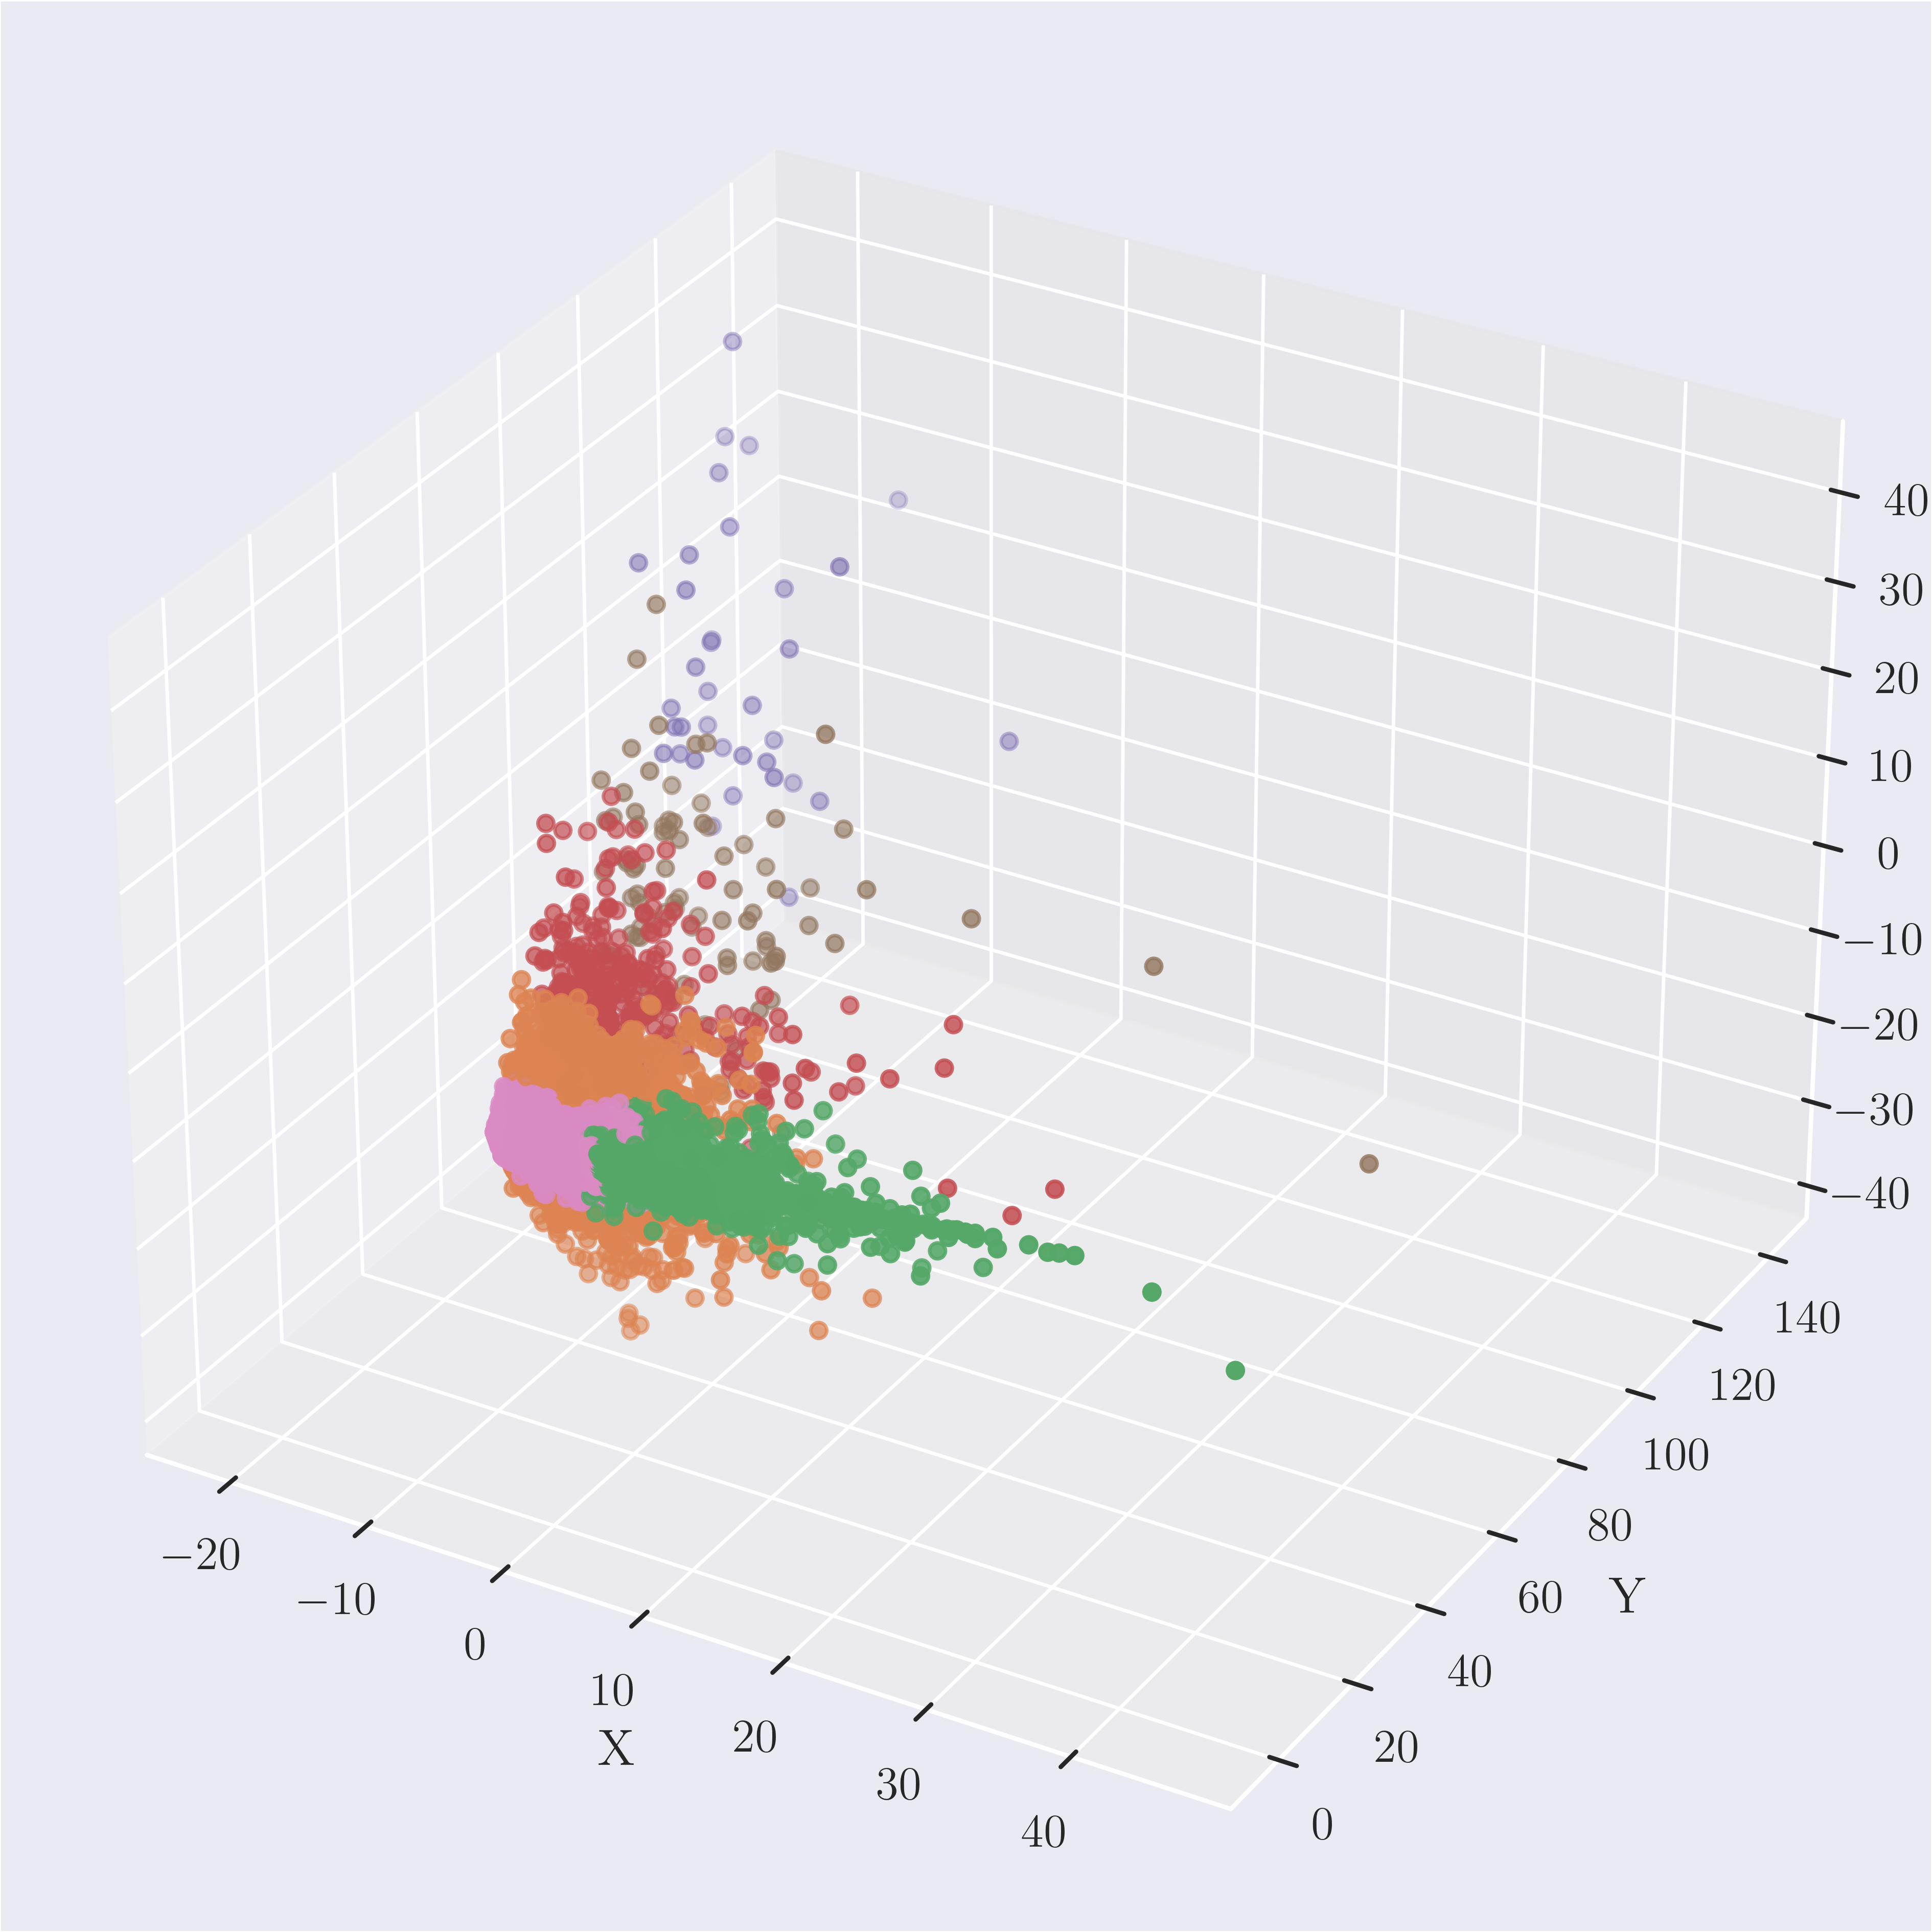
\includegraphics[width=0.99\textwidth]{3d_brc_agn}
        \subcaption{BIRCH+AGNES}
        \label{fig:013-c}
    \end{minipage}
    \caption{PCA三维散点图}
    \label{fig:013}
\end{figure}

\begin{figure}[!htbp]
    \centering
    \begin{minipage}[c]{0.27\textwidth}
        \centering
        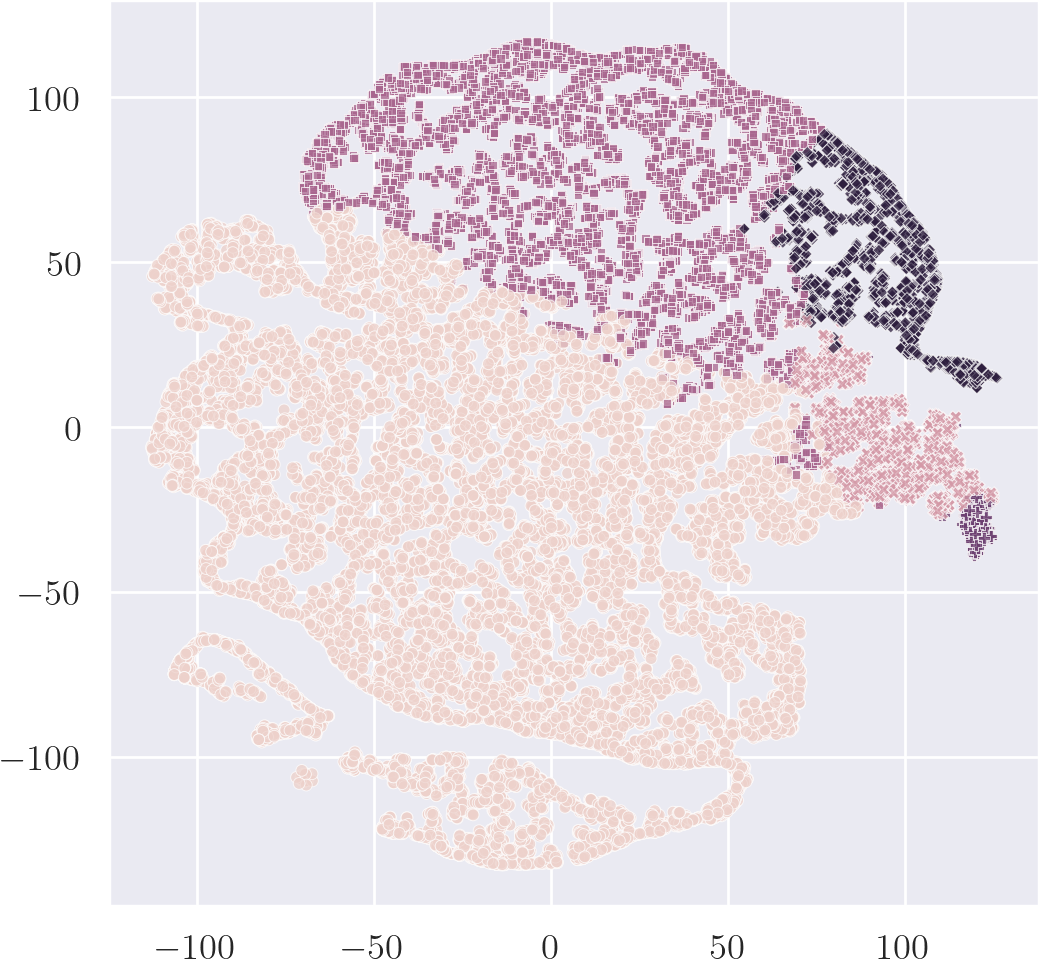
\includegraphics[width=0.99\textwidth]{2d_kmeans}
        \subcaption{K-Means++}
        \label{fig:014-a}
    \end{minipage}
    \begin{minipage}[c]{0.27\textwidth}
        \centering
        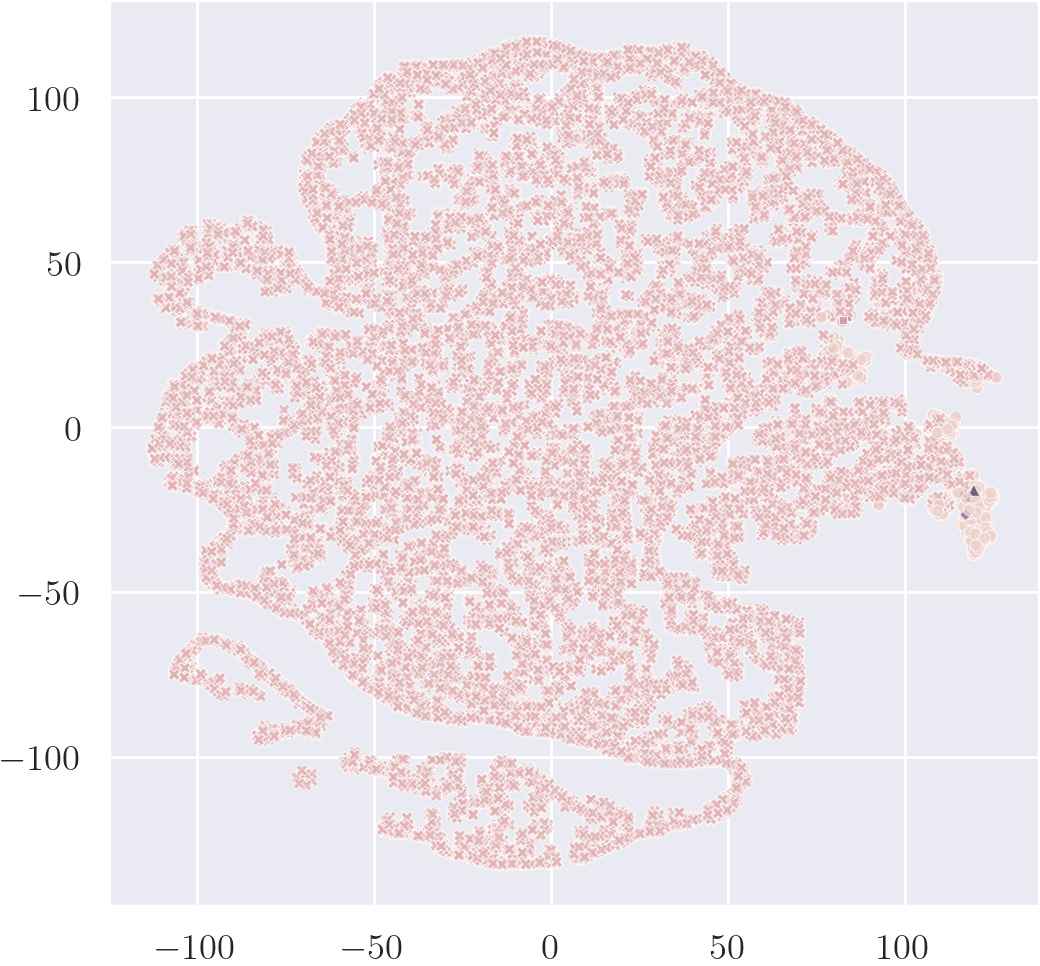
\includegraphics[width=0.99\textwidth]{2d_dbscan}
        \subcaption{DBSCAN}
        \label{fig:014-b}
    \end{minipage}
    \begin{minipage}[c]{0.27\textwidth}
        \centering
        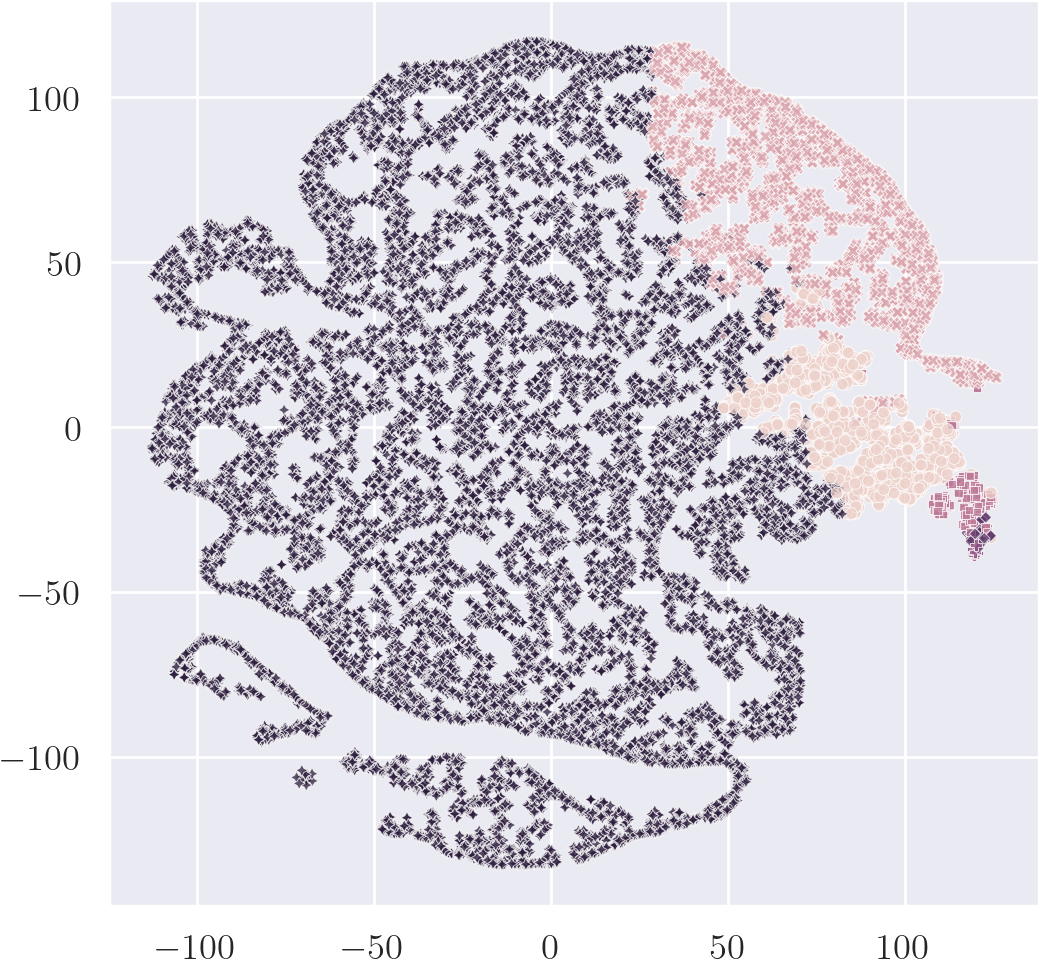
\includegraphics[width=0.99\textwidth]{2d_brc_agn}
        \subcaption{BIRCH+AGNES}
        \label{fig:014-c}
    \end{minipage}
    \caption{t-SNE二维散点图}
    \label{fig:014}
\end{figure}

散点图显示DBSCAN聚类较为笼统,K-Means++与BIRCH+AGNES类间区隔更清晰;从\cref{tab:007}~看,K-Means++更优,故根据K-Means++聚类结果对各用户群体画像。

\subsubsection{用户画像}

根据聚类结果进行数据可视化,可以获得5号人群对20种APP使用时长排序:

$A$类APP:2号 $\approx$ 0号 $\ge$ 1号 $\approx$ 4号 $\ge$ 3号

$B$类APP:2号 $\approx$ 0号 $\ge$ 4号 $\ge$ 1号 $\ge$ 3号

$C$类APP:3号 $\approx$ 1号 $\ge$ 2号 $\approx$ 0号 $\ge$ 4号

$D$类APP:0号 $\ge$ 2号 $\ge$ 1号 $\approx$ 4号 $\ge$ 3号

$E$类APP:0号 $\ge$ 2号 $\ge$ 1号 $\approx$ 4号 $\ge$ 3号

$F$类APP:4号 $\ge$ 2号 $\ge$ 1号 $\approx$ 3号 $\ge$ 0号

$G$类APP:2号 $\ge$ 0号 $\ge$ 1号 $\approx$ 4号 $\ge$ 3号

$H$类APP:2号 $\ge$ 0号 $\ge$ 1号 $\approx$ 4号 $\ge$ 3号

$I$类APP:2号 $\ge$ 0号 $\ge$ 4号 $\approx$ 1号 $\ge$ 3号

$J$类APP:2号 $\ge$ 0号 $\ge$ 4号 $\approx$ 1号 $\ge$ 3号

$K$类APP:2号 $\approx$ 0号 $\approx$ 4号 $\approx$ 1号 $\ge$ 3号

$L$类APP:2号 $\approx$ 0号 $\approx$ 4号 $\approx$ 1号 $\approx$ 3号

$M$类APP:2号 $\approx$ 0号 $\ge$ 4号 $\approx$ 1号 $\approx$ 3号

$N$类APP:2号 $\approx$ 0号 $\ge$ 4号 $\approx$ 1号 $\ge$ 3号

$O$类APP:2号 $\approx$ 0号 $\approx$ 4号 $\approx$ 1号 $\ge$ 3号

$P$类APP:2号 $\approx$ 4号 $\ge$ 0号 $\approx$ 1号 $\ge$ 3号

$Q$类APP:2号 $\approx$ 0号 $\ge$ 4号 $\approx$ 1号 $\ge$ 3号

$R$类APP:2号 $\approx$ 0号 $\ge$ 4号 $\approx$ 1号 $\ge$ 3号

$S$类APP:2号 $\approx$ 0号 $\approx$ 4号 $\ge$ 1号 $\ge$ 3号

$T$类APP:2号 $\approx$ 0号 $\ge$ 4号 $\approx$ 1号 $\ge$ 3号
\begin{figure}[!htbp]
    \centering
    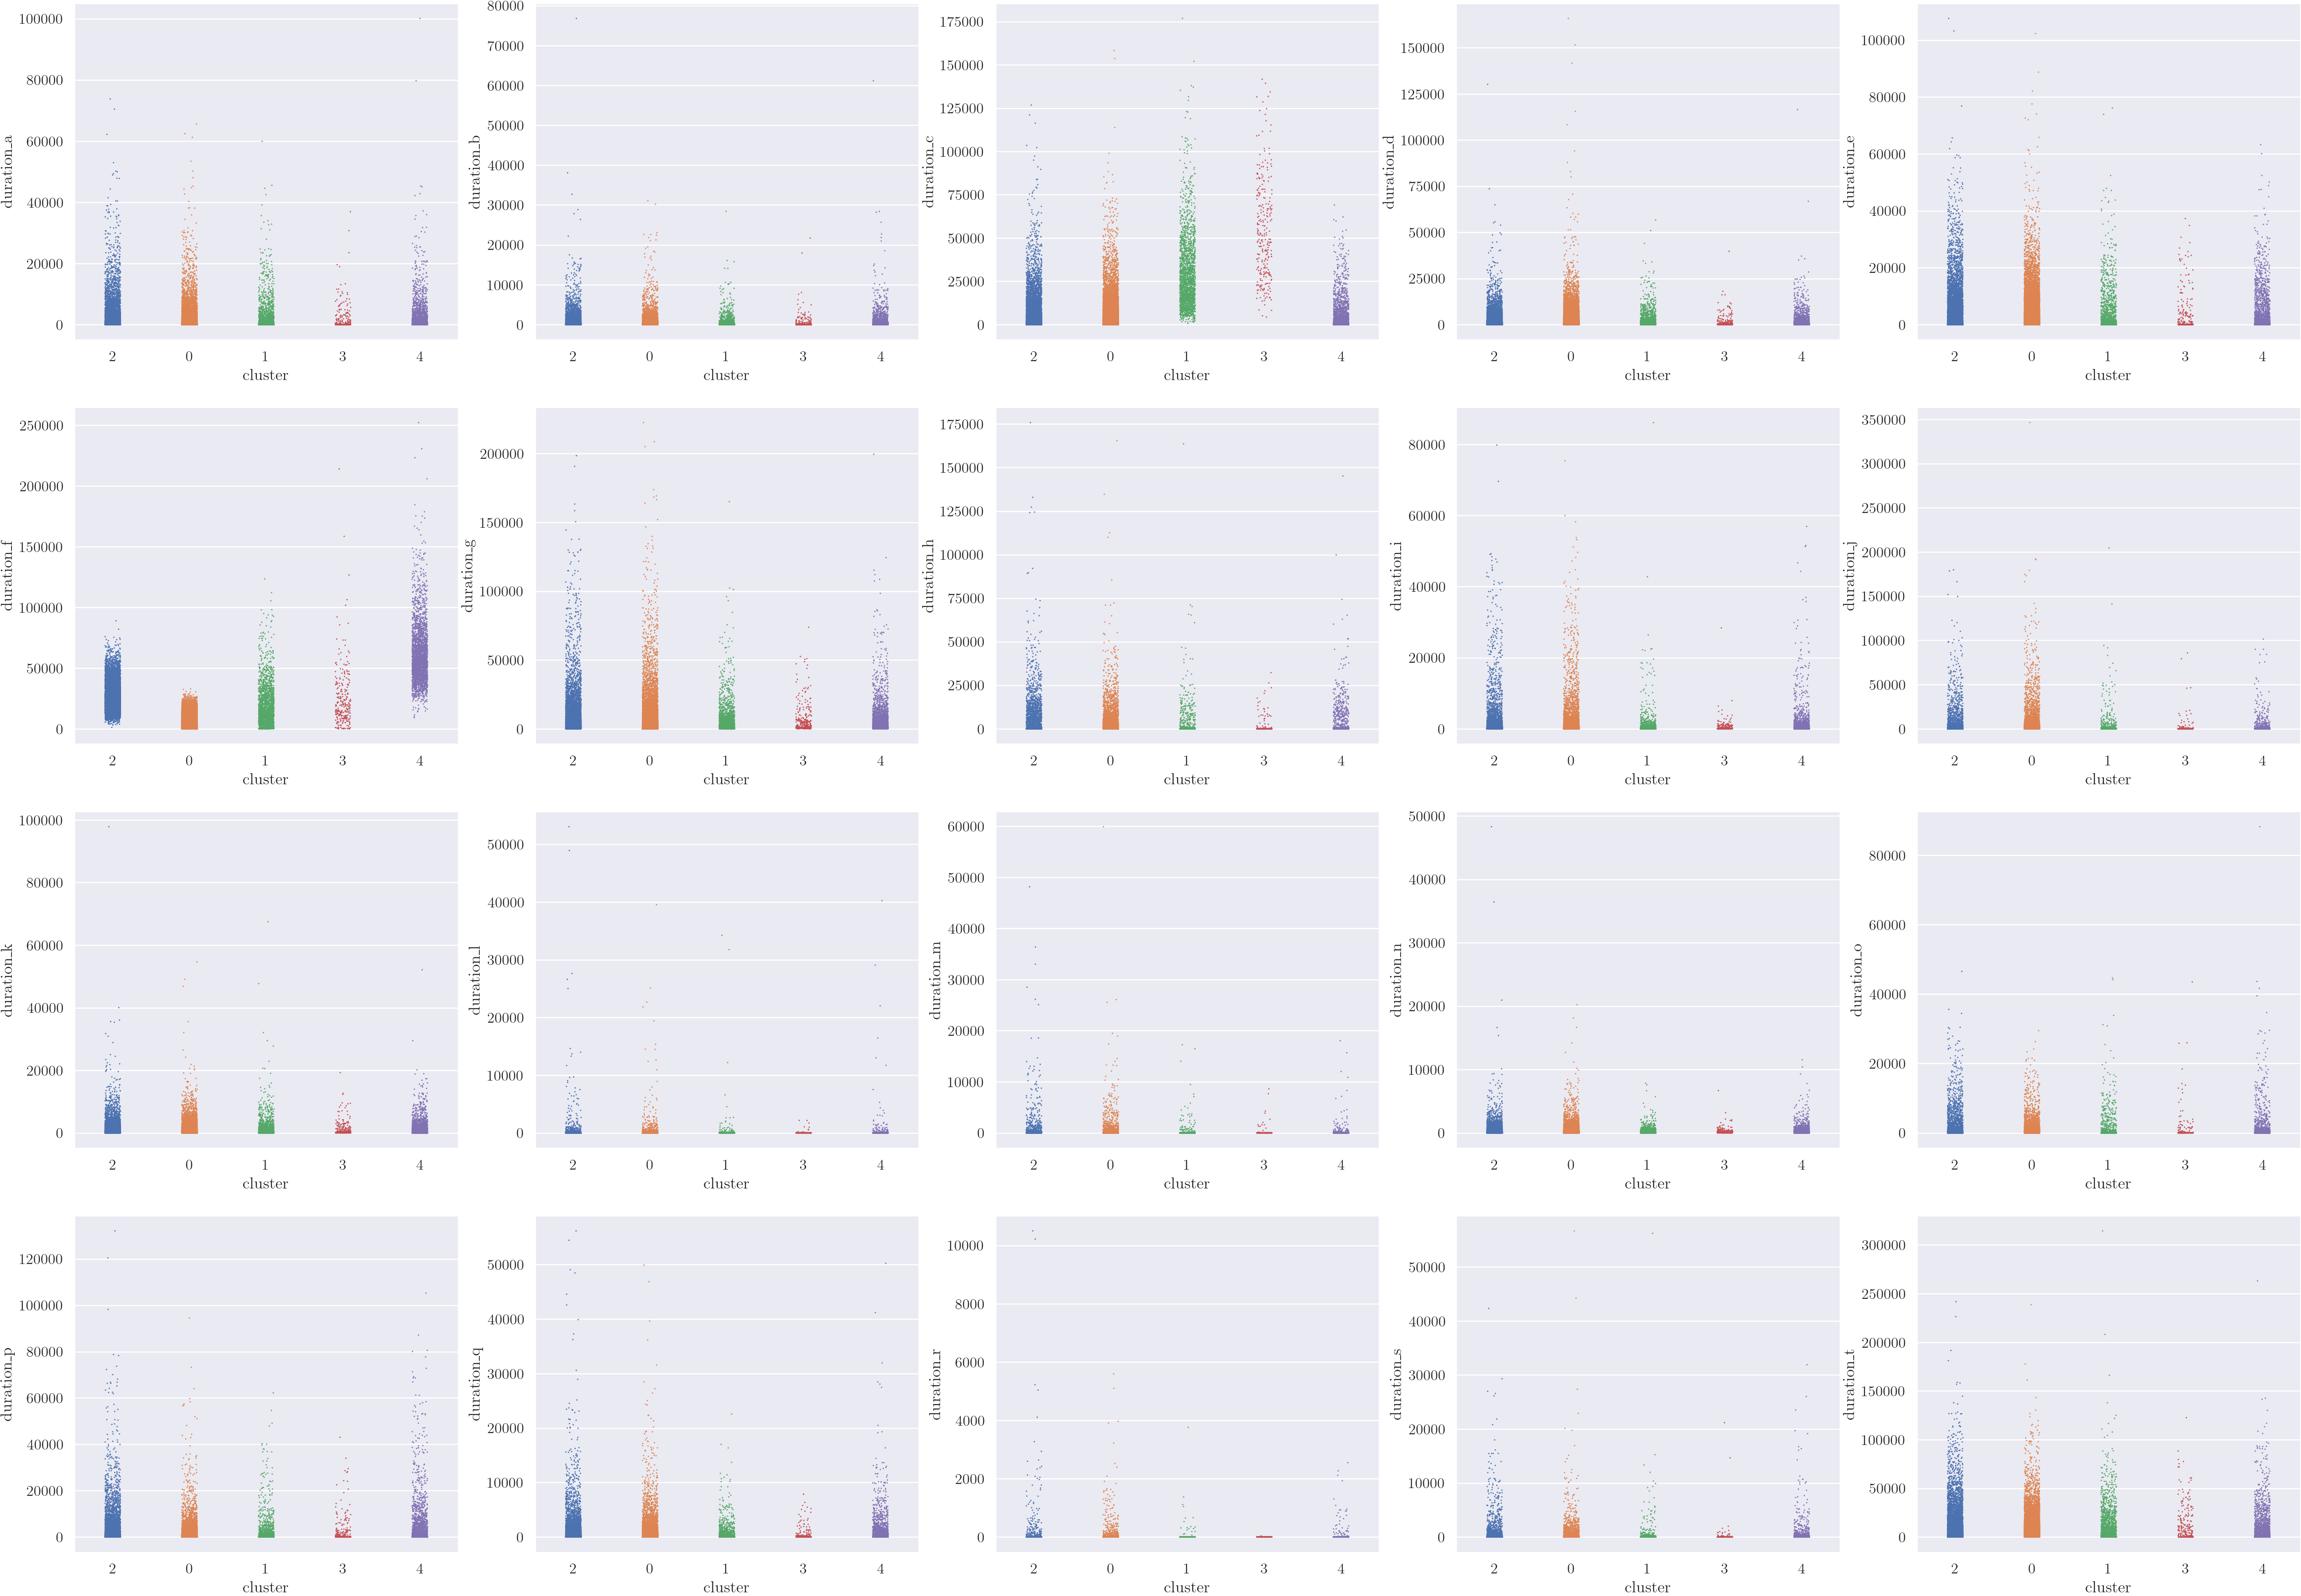
\includegraphics[width=.9\textwidth]{stripplot_duration_cluster}
    \caption{使用时长}
    \label{fig:015}
\end{figure}

\begin{figure}[!htbp]
    \centering
    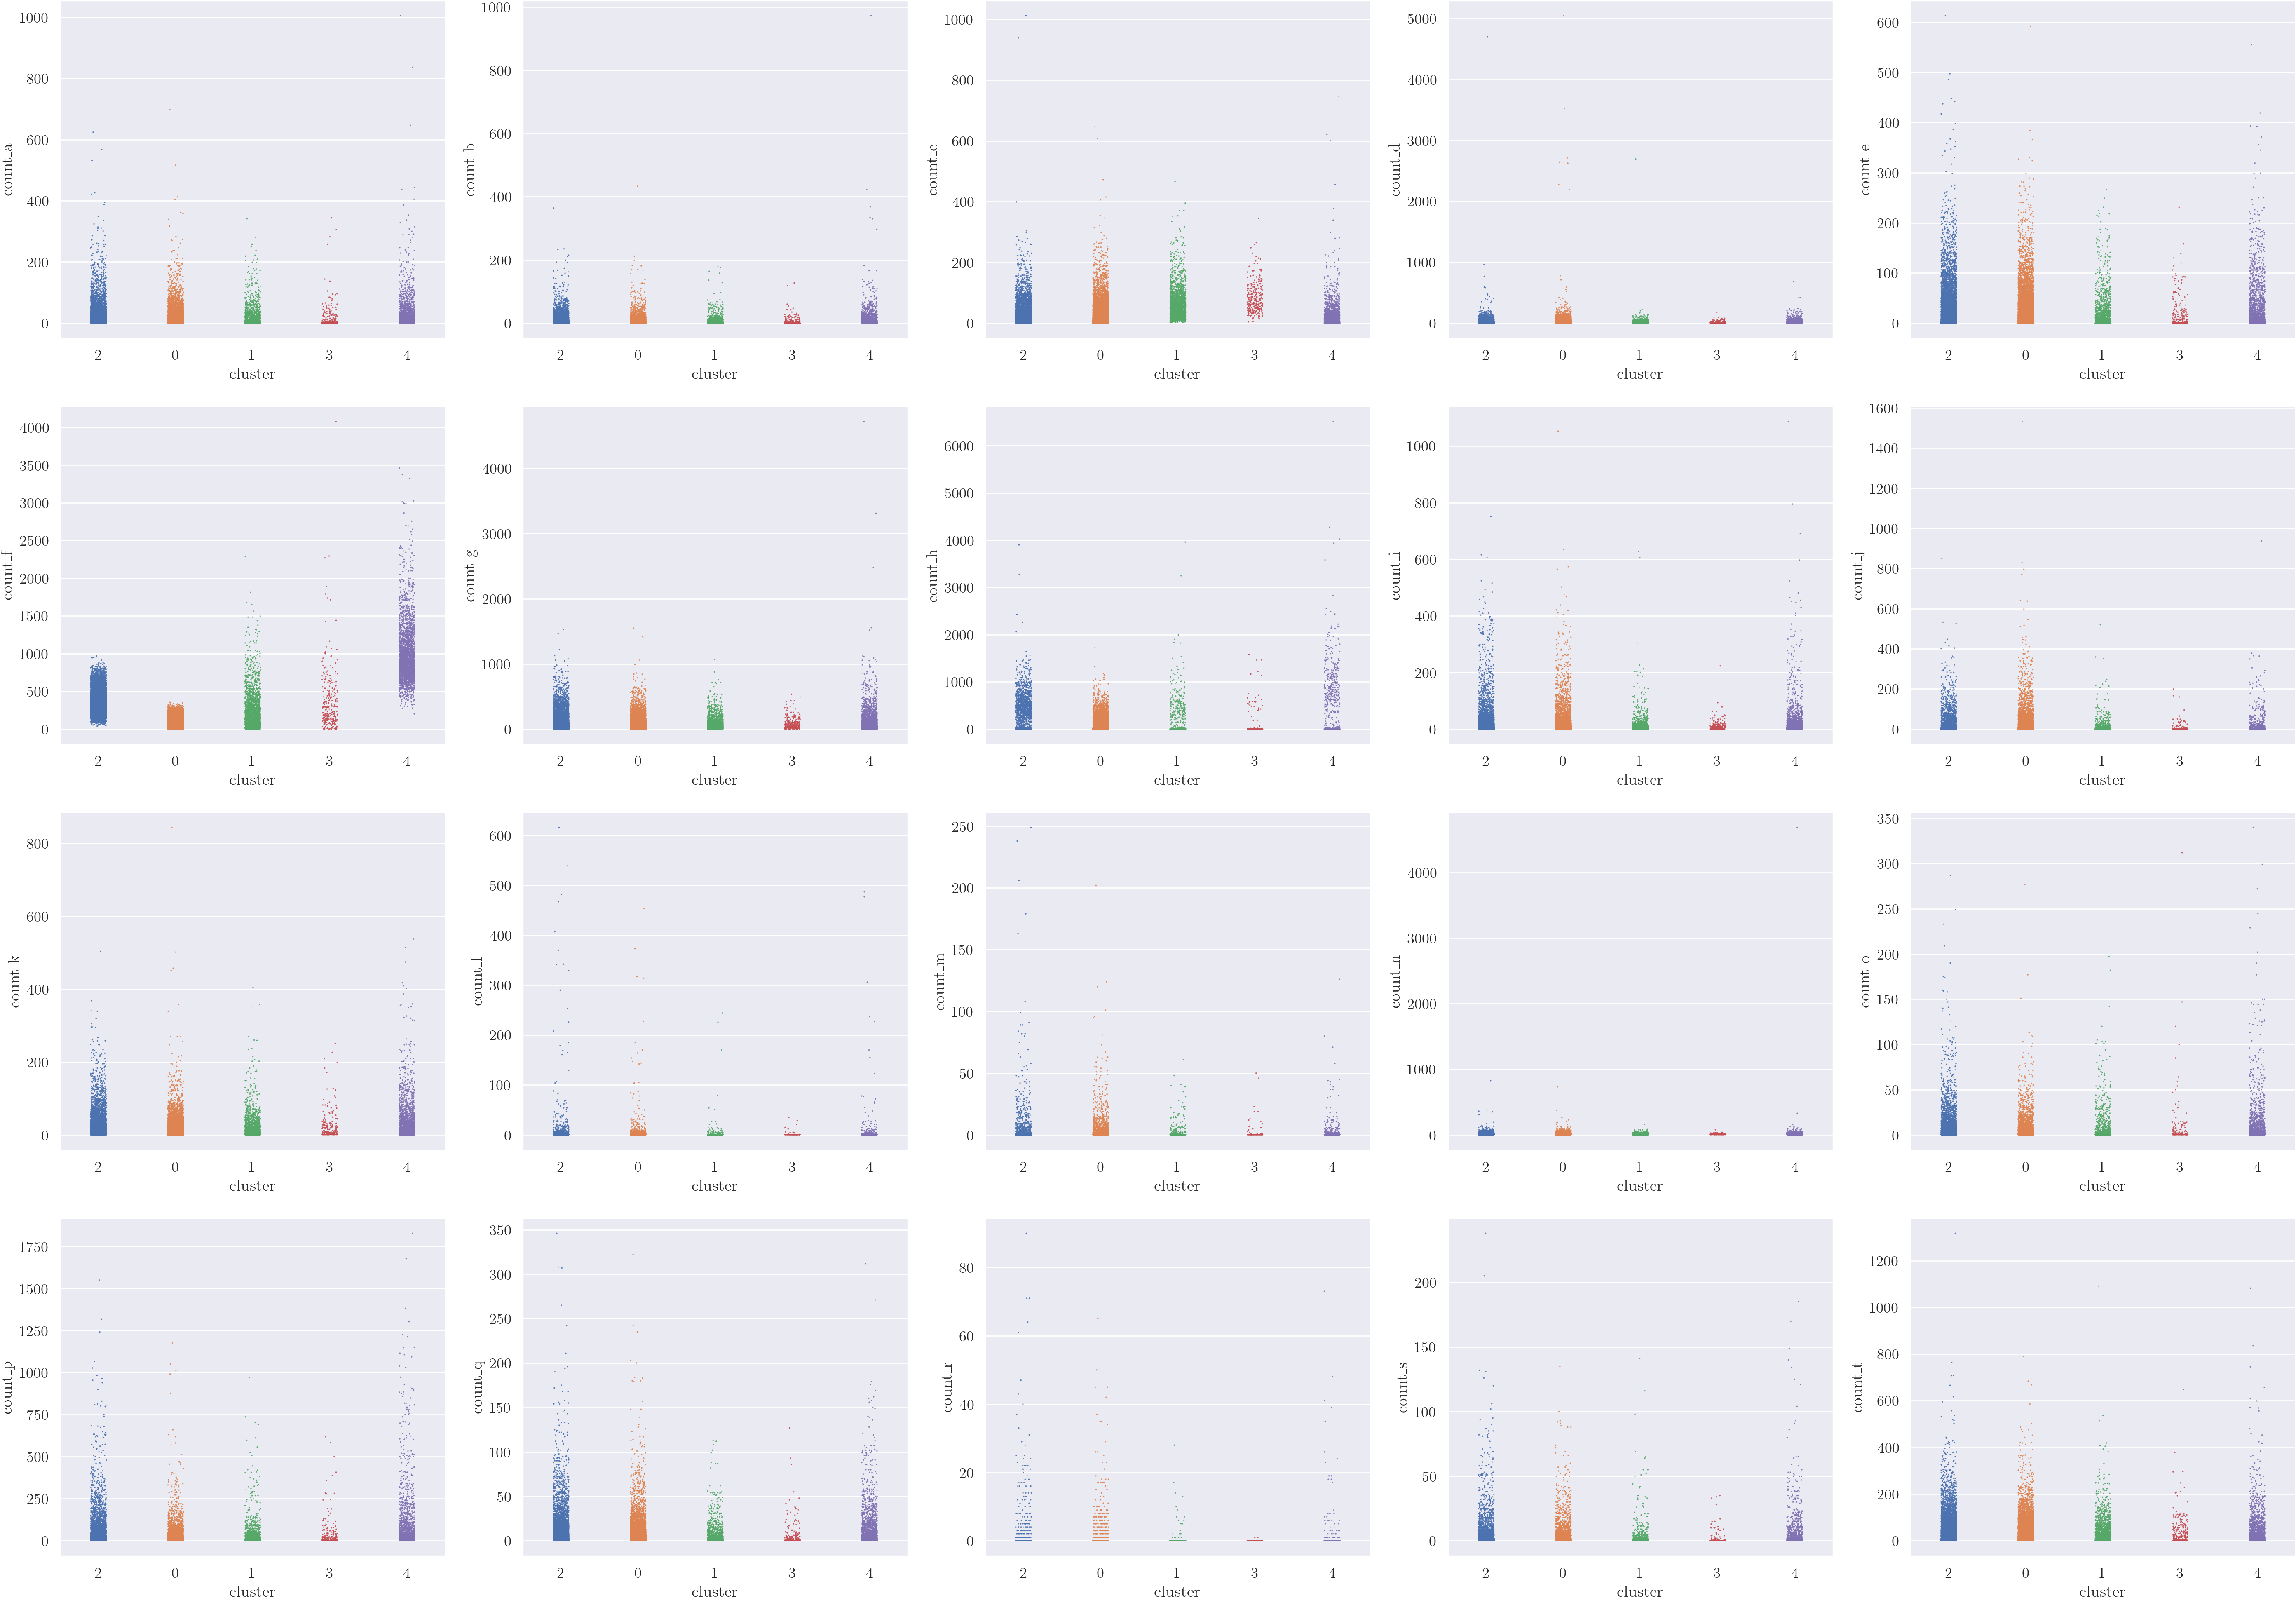
\includegraphics[width=.9\textwidth]{stripplot_count_cluster}
    \caption{使用频次}
    \label{fig:016}
\end{figure}

\begin{figure}[!htbp]
    \centering
    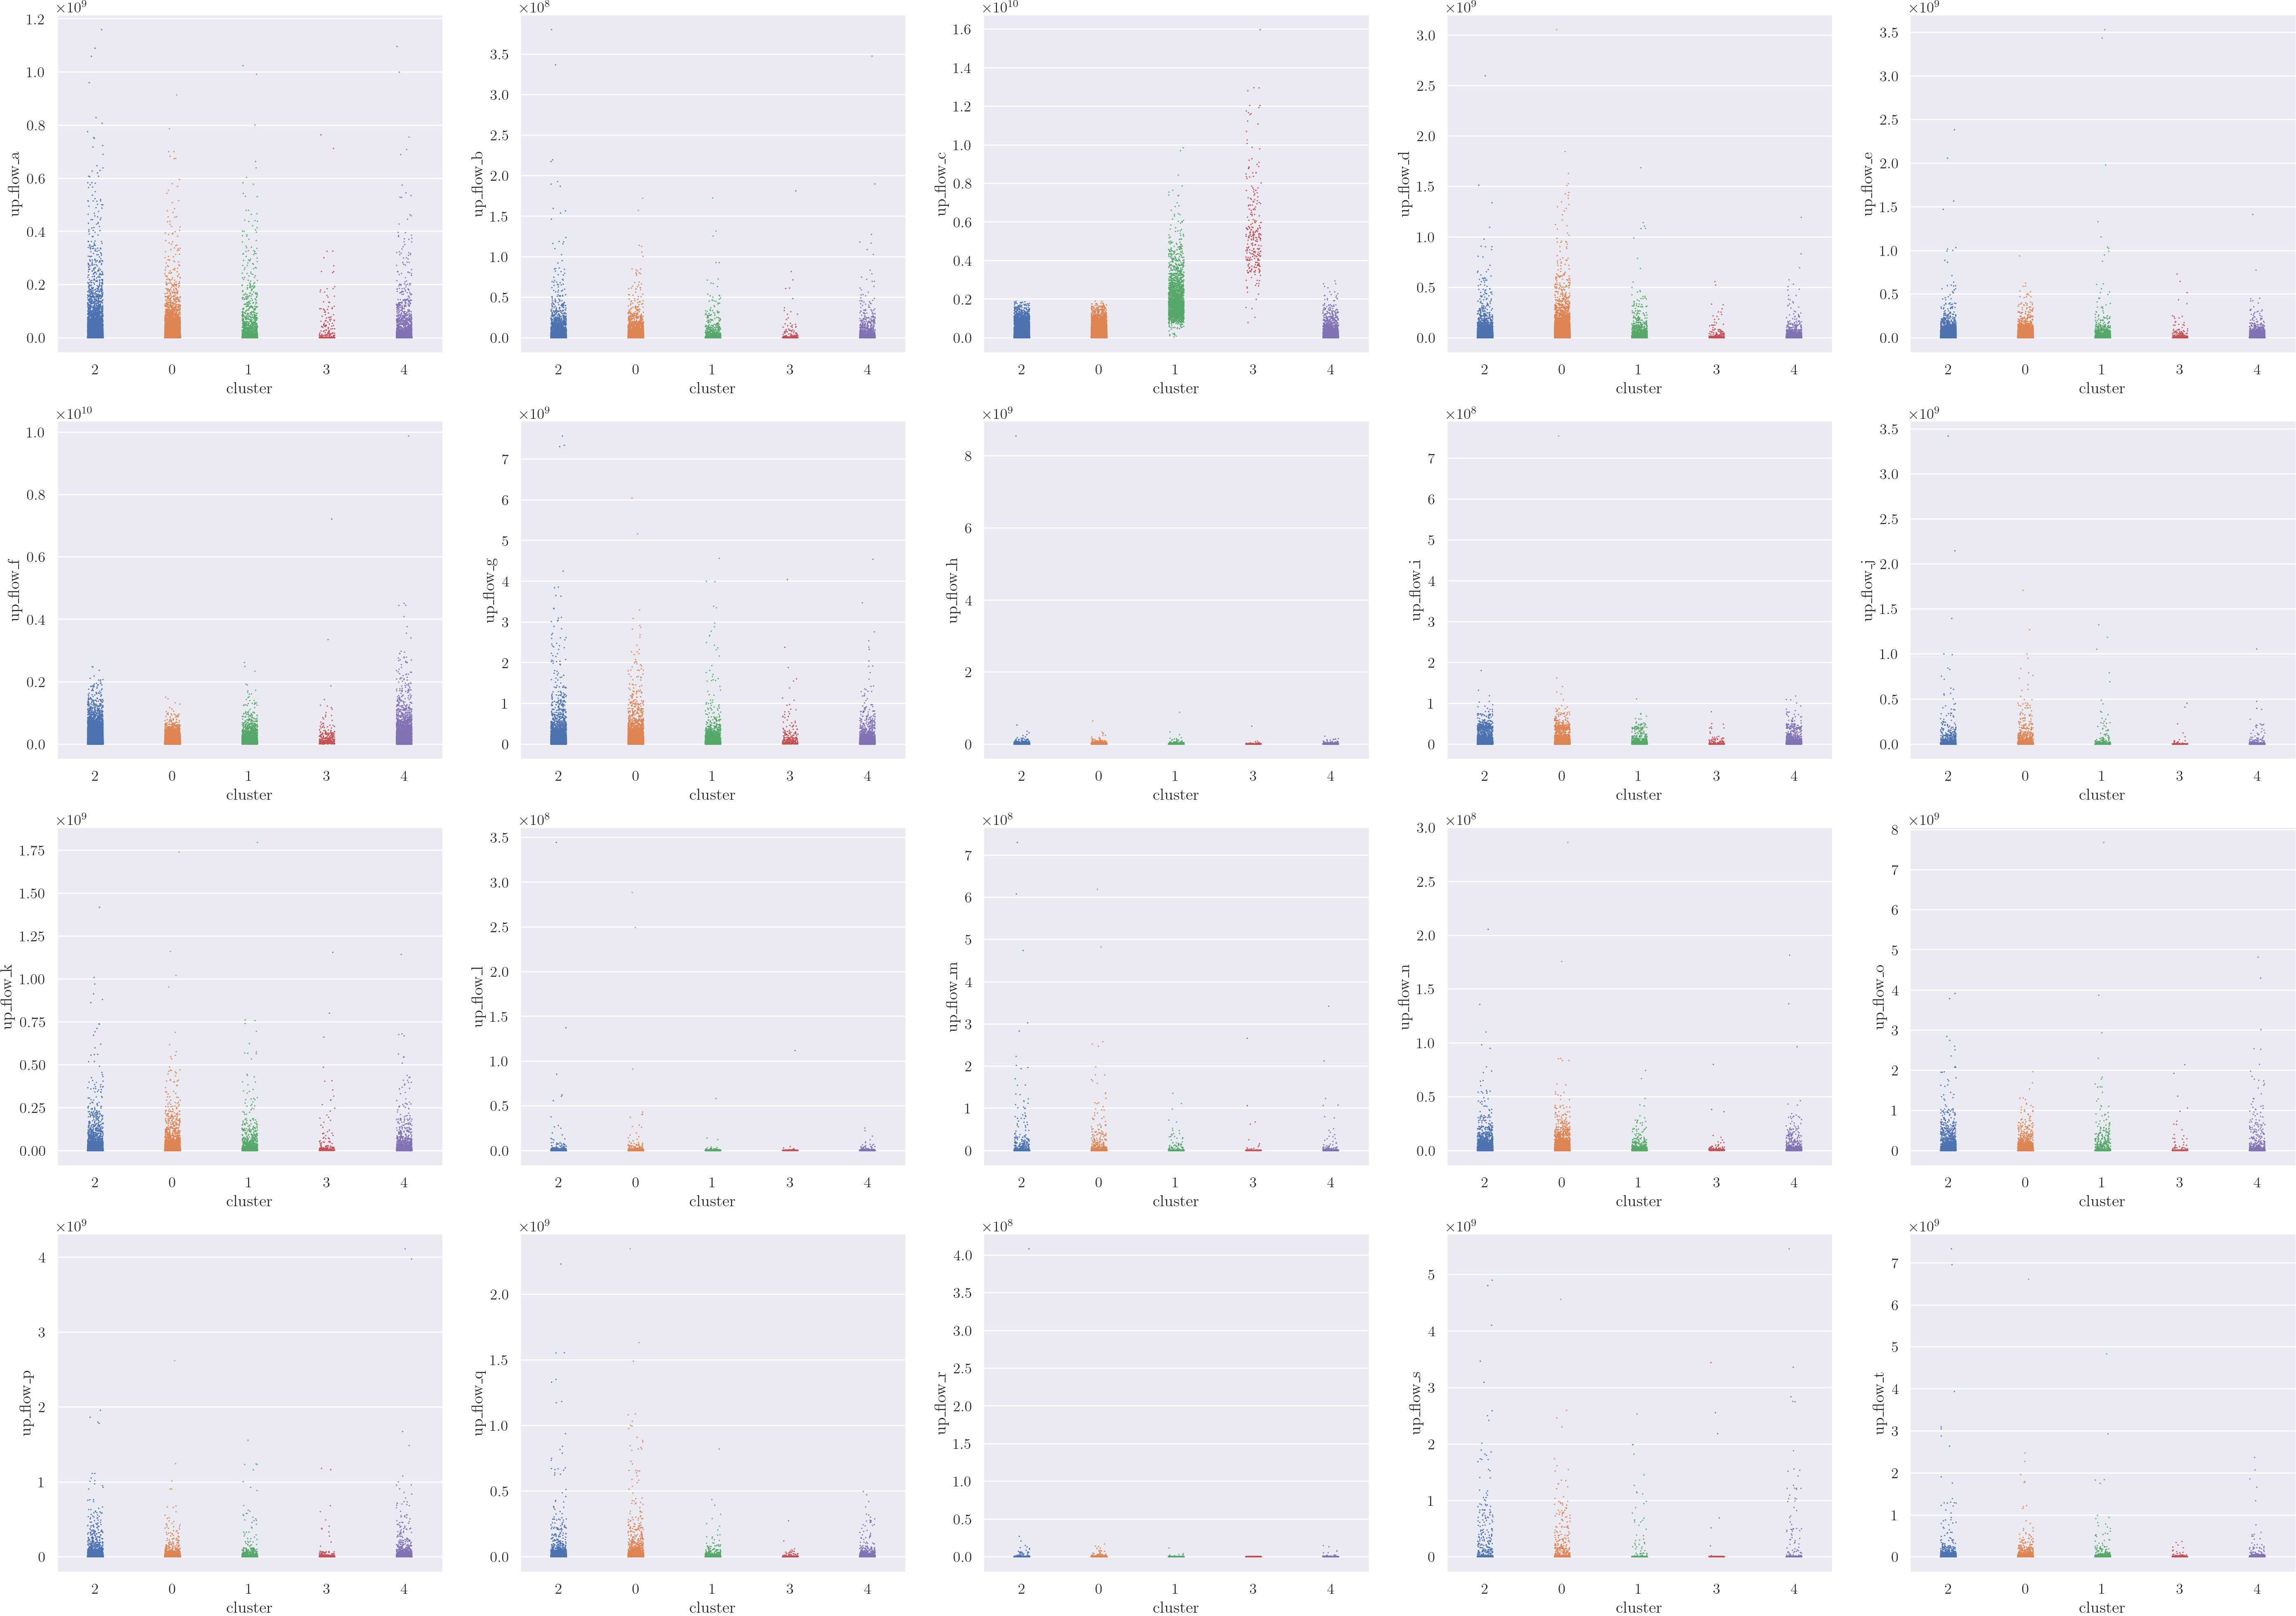
\includegraphics[width=.9\textwidth]{stripplot_up_flow_cluster}
    \caption{上行流量}
    \label{fig:018}
\end{figure}

\begin{figure}[!htbp]
    \centering
    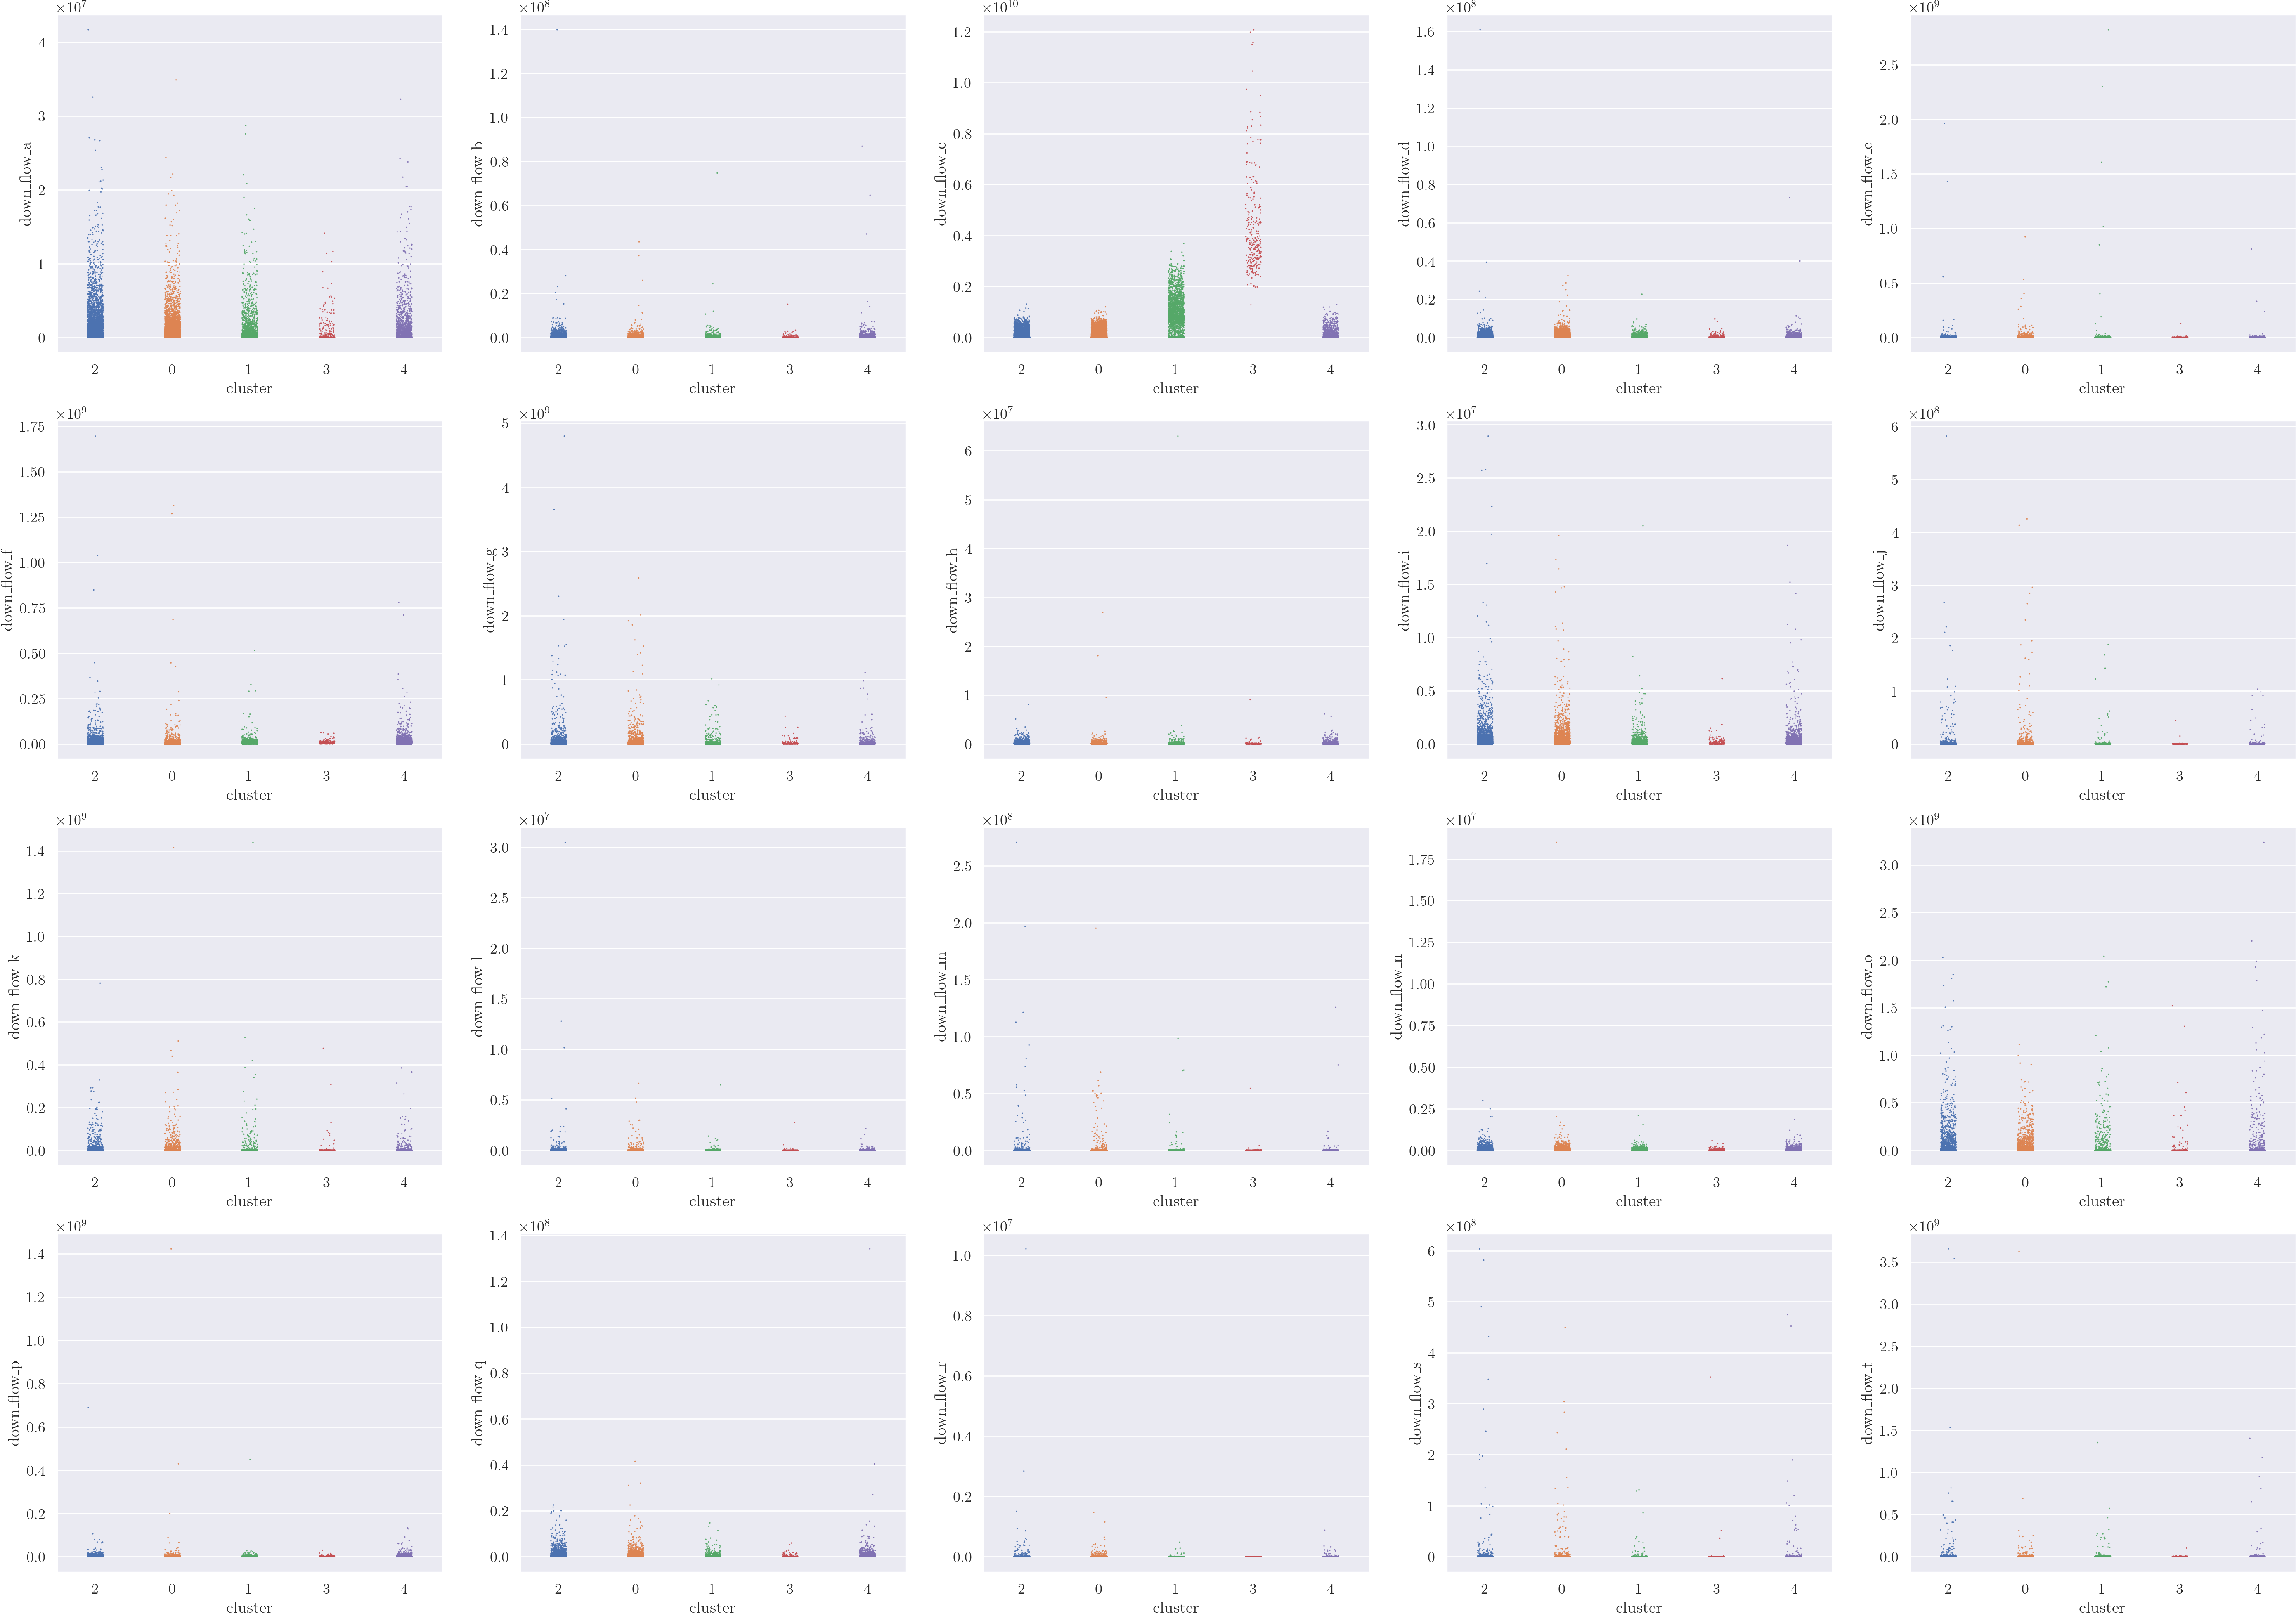
\includegraphics[width=.9\textwidth]{stripplot_down_flow_cluster}
    \caption{下行流量}
    \label{fig:019}
\end{figure}

就\cref{fig:008}~总体情况而言,4号用户群使用智能手机的频次最高,使用时长较高,可能需要时刻刷新手机;0号用户群使用智能手机的频次最低,时长最短,对手机依赖程度不强;1号、3号用户群使用流量最多;相对于4号而言,3号用户群不经常刷新手机,单次使用APP时间较长。

\begin{table}[!htbp]
    \caption{聚类各簇用户统计描述}\label{tab:008} \centering
    \begin{tabular}{lrrrr}
        \toprule[1.5pt]
        $cluster$ & $count\_sum$ & $duration\_sum$ & $up\_flow\_sum$ & $down\_flow\_sum$ \\
        \midrule[1pt]
        0         & 375.776880   & 43624           & 392653844       & 65333138          \\
        1         & 1177.867654  & 159571          & 5290795162      & 2128662377        \\
        2         & 1342.008467  & 122244          & 1131347214      & 167123031         \\
        3         & 1573.553903  & 232744          & 12630933652     & 8764644593        \\
        4         & 2931.083175  & 196532          & 1621400073      & 235777958         \\
        \bottomrule[1.5pt]
    \end{tabular}
\end{table}

就\cref{fig:020}~各类APP情况而言,1号、3号用户群似乎对C类APP“情有独钟”;F类APP使用情况最为参差,4号使用时长最长,降序依次是2号、3号、1号、0号。

\begin{figure}[!htbp]
    \centering
    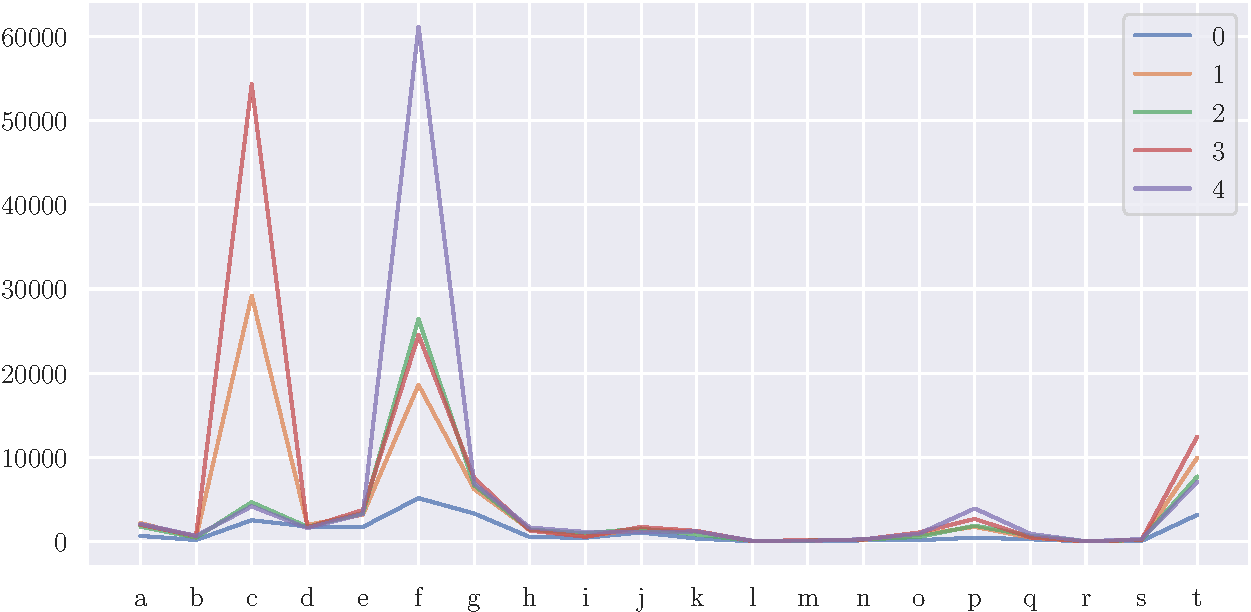
\includegraphics[width=.99\textwidth]{plot_profile}
    \caption{各类用户群对各类APP的使用时长(均值)}
    \label{fig:020}
\end{figure}

\newpage
\section{问题二:未来使用情况预测}

\subsection{评价指标与求解思路}

\subsubsection{评价指标}
对于二元分类任务(第一小问)而言,实际及预测标签输出均为二值变量(真或假,1或0)时,评价指标一般采用混淆矩阵(\cref{fig:confusion}~)定义:

\begin{figure}[!htbp]
    \centering
    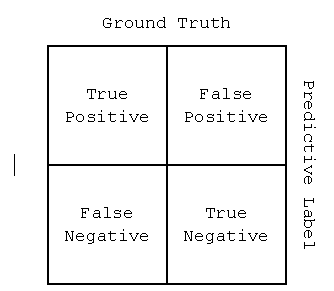
\includegraphics[width=.3\textwidth]{confusion}
    \caption{混淆矩阵}
    \label{fig:confusion}
\end{figure}

准确率(accuracy)表示正确预测的比率,表示预测正确的数据占所有资料的比率:
\begin{equation}
    acc = \frac{TP+TN}{TP+TN+FP+FN}
    \label{eq:acc}
\end{equation}

此外,精准率(precision)、召回率(recall)、调和平均F1值也经常作为评价指标:
\begin{equation}
    prec = \frac{TP}{TP+FP}
    \label{eq:prec}
\end{equation}

\begin{equation}
    recall = \frac{TP}{TP+FN}
    \label{eq:recall}
\end{equation}

\begin{equation}
    F_1 = \frac{2}{\frac{1}{prec}+\frac{1}{recall}}
    \label{eq:f1}
\end{equation}

对于回归任务(第二小问)而言,常用评价指标包括均方根误差(RMSE)、均方根对数误差(RMSLE)、平均绝对值误差(MAE)、决定系数($R^2$)等,本题采用NMSE:

\begin{equation}
    RMSE = \sqrt[]{
        \frac{1}{N} \sum_{i=1}^{N} (y_i-\hat{y_i})^2
    }
    \label{eq:rmse}
\end{equation}

\begin{equation}
    RMSLE = \sqrt[]{
    \frac{1}{N} \sum_{i=1}^{N} (\log(1+y_i)-\log(1+\hat{y_i}))^2
    }
    \label{eq:rmsle}
\end{equation}

\begin{equation}
    MAE = \frac{1}{N} \sum_{i=1}^{N} |y_i-\hat{y_i}|
    \label{eq:mae}
\end{equation}

\begin{align}
    R^2     & = 1- \frac{
        \sum_{i=1}^{N} (y_i-\hat{y_i})^2}{
    \sum_{i=1}^{N} (y_i-\bar{y_i})^2}         \\
    \bar{y} & =\frac{1}{N} \sum_{i=1}^{N} y_i
    \label{eq:r2}
\end{align}

\begin{equation}
    NMSE = \sqrt[]{\frac{
            \sum_{i=1}^{N} (y_i-\hat{y_i})^2}{
            \sum_{i=1}^{N} (y_i-\bar{y_i})^2}}
    \label{eq:nmse}
\end{equation}

公式中符号意义如下:

\begin{table}[!htbp]
    \caption{评价指标符号意义}\label{tab:equation} \centering
    \begin{tabular}{ccccc}
        \toprule[1.5pt]
        符号          & 意义                                            \\
        \midrule[1pt]
        $N$         & 资料笔数,本题代表1~21天出现的用户总数                         \\
        $i$         & $1, 2,\ldots, N$,为每笔资料的索引                     \\
        $y_i$       & 第$i$笔资料的实际值,如第$i$名用户第12至21天使用a类APP的实际有效日均使用时长 \\
        $\hat{y_i}$ & 第$i$笔资料的预测值,如第$i$名用户第12至21天使用a类APP的预测有效日均使用时长 \\
        \bottomrule[1.5pt]
    \end{tabular}
\end{table}

\subsubsection{系统Pipeline}

在使用机器学习建立模型解决第一小问与第二小问前,必须先确定模型输入与输出的固定格式与含义。从系统本身而言,问题二要求输入1~11天用户使用APP监测数据,输出12~21天用户是否使用A类APP以及日均使用时长。这一问题兼具“用户行为属性”与“时间序列属性”,我们可以将这一复杂问题在两个方向进行抽象、简化:

\begin{enumerate}
    \item 输入某用户前一天是否使用A类APP(类别),输出该用户后$1$天是否使用(类别)
    \item 输入某用户前$n$天是否使用A类APP(向量),输出该用户后$1$天是否使用(类别)
    \item 输入某用户前$n$天是否使用A类APP(向量),输出该用户后$n$天是否使用(向量)
    \item 输入某用户前$1$天的使用时长(标量),输出一个用户后$1$天的使用时长(标量)
    \item 输入某用户前$n$天的使用时长(向量),输出一个用户后$1$天的使用时长(标量)
    \item 输入某用户前$n$天的使用时长(向量),输出一个用户后$n$天的使用时长(向量)
\end{enumerate}

由于12~21天属于测试集,不可泄漏参与训练,因此天然缺失构建$n=10$的6号、3号求解框架,如果选取$n=3$或许不符合以7天为周期的社会性活动常识。因此,本文折衷资料数目与特征数目,提出了两种求解框架进行模式识别、特征挖掘:
\begin{enumerate}
    \item 输入某用户前$n$天的使用时长(向量),输出一个用户后$1$天的使用时长(标量),并通过预训练模型执行上游任务:滑动窗口覆盖21天,如\cref{fig:pipeline1}。
    \item 输入某用户前$n$天的使用时长(向量),输出一个用户后$m$天的使用时长(向量),并通过预训练模型执行上游任务:滑动窗口覆盖21天,如\cref{fig:pipeline2}。
\end{enumerate}

\begin{figure}[!htbp]
    \centering
    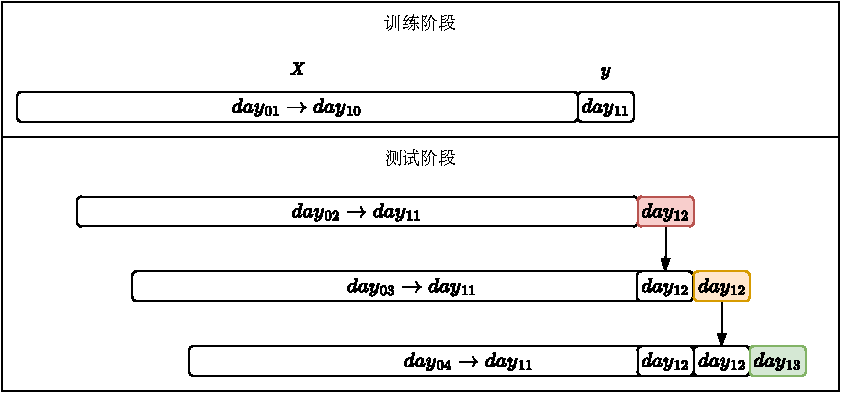
\includegraphics[width=.85\textwidth]{pipeline1}
    \caption{求解框架(一)}
    \label{fig:pipeline1}
\end{figure}

\begin{figure}[!htbp]
    \centering
    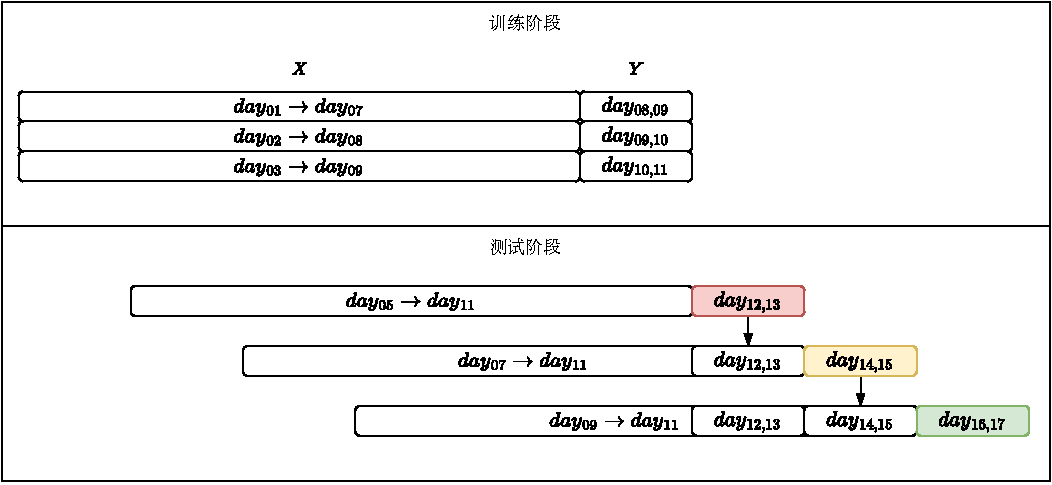
\includegraphics[width=.85\textwidth]{pipeline2}
    \caption{求解框架(二)}
    \label{fig:pipeline2}
\end{figure}

对于提出的两种求解框架,考虑到实现细节与篇幅页数的限制,下文仅讨论和展示框架(一),根据监测数据每日A类APP有效使用时长作为特征建立训练集、测试集,共计47345笔资料。

\subsection{超参数选择与预训练模型建立}

\subsubsection{建立KNN最近邻分类预测模型}

KNN将无类别标签样本归为最接近该点的$K$个样本点中最频繁使用的一类。本文在1~40所有奇数中,对$K$值进行网格搜索,在训练资料上对模型采用8折交叉验证,运行结果显示:$K=33$时,正确率最高可达$87.508\%$。

\subsubsection{建立LogisticRegression分类预测模型}

LogisticRegression也称“对数概率回归”,属于一种基于概率的判别模型。
在训练资料上对模型采用8折交叉验证,运行结果显示:模型在预训练资料上正确率平均为$87.31\%$。

\subsubsection{建立随机森林集成分类预测模型}

随机森林是一个集成装箱多个决策树的分类器,每棵树模型采用Bootstrap方式对特征进行采样。
本文对\cref{tab:010}~三类超参数进行网格搜索,在训练资料上对模型采用3折交叉验证,运行结果显示,设置下列超参数时,正确率最高可达$88.71\%$。

\begin{table}[!htbp]
    \caption{随机森林最佳超参数}\label{tab:010} \centering
    \begin{tabular}{cccccc}
        \toprule[1.5pt]
        超参数             & 取值 & 超参数                  & 取值 & 超参数          & 取值 \\
        \midrule[1pt]
        $n\_estimators$ & 60 & $min\_samples\_leaf$ & 7  & $max\_depth$ & 12 \\
        \bottomrule[1.5pt]
    \end{tabular}
\end{table}

\subsubsection{建立XGBoost集成回归预测模型}

XGBoost也是以决策树为基础的模型,采用梯度提升对多棵决策树进行组合,在准确率、运算速度、操作便利性上表现优秀。采用网格搜素超参数,在训练资料上对模型采用10折交叉验证,选择超参数如\cref{tab:011}时,在预训练资料上(给定1~10天,预测第11天)NMSE损失最小可达$1.52$。

\begin{table}[!htbp]
    \caption{XGBoost最佳超参数}\label{tab:011} \centering
    \begin{tabular}{cccccc}
        \toprule[1.5pt]
        超参数             & 取值 & 超参数          & 取值 & 超参数                  & 取值  \\
        \midrule[1pt]
        $n\_estimators$ & 30 & $max\_depth$ & 7  & $min\_child\_weight$ & 1.0 \\
        \bottomrule[1.5pt]
    \end{tabular}
\end{table}

\subsection{运行结果与改进方向}
\subsubsection{运行结果}

对于上游任务一“预测第12~21天是否会使用该类APP”,采用随机森林算法以第12天预测结果作为12~21天的代表,正确率仅有$68.4\%$。

对于上游任务二“预测第12~21天用户使用a类APP的有效日均使用时长”,采用XGBoost算法以滑动窗的形式依次获得12~21天A类APP每日有效使用时长,而后获得平均日均使用时长,NMSE低至0.932。

\subsubsection{改进方向}

未来的改进措施可以考虑将回归问题退化为分类问题,选择合适的阈值,当阈值大于某设定值时,记为使用该类APP,否则视为无效使用。同时,可以考虑Voting、Stacking等集成方式进一步提升模型效能。

%参考文献
\newpage
\begin{thebibliography}{9}
    \bibitem{机器学习} 周志华. 机器学习[M]. 北京. 清华大学出版社. 2016. 197-219
    \bibitem{高维数据的聚类分析} 何宏. 高维数据的聚类分析[M]. 上海. 上海交通大学出版社. 2022. 1-16
    \bibitem{数据仓库与数据挖掘} 陈志泊,韩慧,王建新,孙俏,聂耿青. 数据仓库与数据挖掘[M]. 北京. 清华大学出版社. 2009
    \bibitem{常乐} 常乐. 基于用户行为分析的用户画像系统设计与实现[D]. 北京邮电大学. 2020
    \bibitem{陈纯} 陈纯,龙瀛,黄贵恺. 屏幕使用时间与步行活动关系的探索性研究[J]. 景观设计学(中英文). 2021. 9(04):68-81
    \bibitem{成雪} 成雪,于冬梅,赵丽云等. 2016—2017年中国各省中小学生电子屏幕使用现状[J]. 卫生研究. 2023,52(03):382-387
    \bibitem{武慧娟} 武慧娟,赵天慧,孙鸿飞等. 基于支付意愿的数字阅读用户画像聚类研究[J]. 情报科学. 2022. 40(05)
    \bibitem{侯金凤} 侯金凤. 移动互联网下手机用户使用行为特征的研究[J]. 电脑知识与技术. 2016,12(07)
    \bibitem{韦磊} 韦磊. 基于移动终端数据的用户画像模型研究[D]. 江苏科技大学. 2021
    \bibitem{timeseries} Garg, R., \& Barpanda, S. Machine Learning Algorithms for Time Series Analysis and Forecasting[Z/OL]. arXiv preprint arXiv:2211.14387. https://arxiv.org/abs/2211.14387
    \bibitem{CH} T. Caliński, J Harabasz. A dendrite method for cluster analysis[J]. Communications in Statistics. 1974. 3:1, 1-27
    \bibitem{DB} Davies D L , Bouldin D W. A Cluster Separation Measure[J]. IEEE Transactions on Pattern Analysis and Machine Intelligence. 1979. PAMI-1(2):224-227
    \bibitem{SC} Peter R J . Silhouettes: A graphical aid to the interpretation and validation of cluster analysis[J]. Journal of Computational \& Applied Mathematics. 1987. 20
    \bibitem{sklearn} Swami A , Jain R. Scikit-learn: Machine Learning in Python[J]. Journal of Machine Learning Research. 2013, 12(10):2825-2830
    \bibitem{birch} Zhang T , Ramakrishnan R. Miron Livny: BIRCH: An Efficient Data Clustering Method for Very Large Databases[J]. ACM SIGMOD Record. 1999. 25(2)
    \bibitem{birch2} 赵玉艳,郭景峰,郑丽珍等. 一种改进的BIRCH分层聚类算法[J]. 计算机科学. 2008(03):180-182+208
    \bibitem{eps1} Sander J , Ester M , Kriegel H P ,et al. Density-Based Clustering in Spatial Databases: The Algorithm GDBSCAN and Its Applications[J]. Data Mining \& Knowledge Discovery. 1998. 2(2):169-194
    \bibitem{eps2} Schubert E , Sander J , Ester M ,et al. DBSCAN revisited, revisited: Why and how you should (still) use DBSCAN[J]. ACM Transactions on Database Systems, 2017, 42(3):1-21
    \bibitem{tsne} Maaten L J P V D , Hinton G E. Visualizing High-Dimensional Data using t-SNE[J]. Journal of Machine Learning Research. 2008. 9:2579-2605.
    % \bibitem[6] 论文集: \[序号\] 著者.篇名.主编.论文集名\[C\].出版地.出版者.出版年.起止页码
    % \bibitem[7] 科技报告:\[序号\]著者.题名\[R\]. 报告题名. 编号.出版地.出版者. 出版年.起止页码
    % \bibitem[8] 学位论文:\[序号\] 著者.题名\[D\].保存地点.授予年
    % \bibitem[9] 专利文献:\[序号\] 专利申请者.题名\[P\]. 国别.专利文献种类.专利号.出版日期
\end{thebibliography}
%附录
\newpage
\begin{appendices}

    \section{运行环境与环境依赖}
    代码在Python3.9.12,MacBook Air Apple M1 MacOS13.0.1 (22A400)测试无误。下载解压初赛数据集,将app\_class.csv、dayxx.txt放至Datasets文件夹中,在Visual Studio Code 或 Terminal 中运行 `preprocessing.py`的`generate\_pickle\_origin`,获得pickle格式的粗处理数据,对应2.1、2.2、2.3、2.4小节。

    除数据清洗、预处理源代码直接来自Python脚本,其余附录所列出的代码均由Jupyter Notebook记事本文件导出。
    \begin{lstlisting}[language=Python]
matplotlib~=3.7.2
numpy~=1.23.5
pandas~=2.0.3
scienceplots~=2.1.0
scikit_learn~=1.3.0
seaborn~=0.12.2
tqdm~=4.64.0
xgboost~=1.7.6
ydata_profiling~=4.3.1
    \end{lstlisting}

    \section{数据清洗、预处理源代码}
    \begin{lstlisting}[language=Python]
from tqdm.auto import tqdm
import pandas as pd
import os


def generate_pickle_origin(start_day=1, end_day=21):
    # 读取类型数据
    app = pd.read_csv(
        filepath_or_buffer='../Datasets/app_class.csv',
        header=None
    ).drop_duplicates()

    # 更新列标签
    app.columns = ['appid', 'app_class']

    # 新增一笔虚拟资料(NaN)
    app = pd.concat(
        objs=[pd.DataFrame({"appid": [-404], "app_class": ['NaN']}), app],
        ignore_index=True
    )

    # 约束数据格式
    app['app_class'] = app['app_class'].astype('category')
    app['appid'] = app['appid'].astype('category')

    # 初赛数据集day1~21
    for i in tqdm(range(start_day, end_day + 1)):
        # 读取监测数据
        df = pd.read_csv(
            filepath_or_buffer=f'../Datasets/day{str(i).zfill(2)}.txt',
            header=None
        ).drop_duplicates()

        # 更新列标签
        df.columns = ['uid', 'appid', 'app_type', 'start_day', 'start_time',
                        'end_day', 'end_time', 'duration', 'up_flow', 'down_flow']

        # 新增app_class,对于所属类别未知的APP,类别记作NaN
        df = df.merge(app, on='appid', how='left')
        df['app_class'] = df['app_class'].fillna('NaN')

        # 约束数据格式
        df['appid'] = df['appid'].astype('category')
        df['uid'] = df['uid'].astype('category')
        df['app_type'] = df['app_type'].astype('category')

        # df['start_time'] = pd.to_datetime(df['start_time'], format="%H:%M:%S")
        # df['end_time'] = pd.to_datetime(df['end_time'], format="%H:%M:%S")
        # 使用 pandas.Timestamp 将 `day` 和 `time` 合并
        # df['start_time_new'] = df.apply(
        #     lambda x: x['start_time'] + pd.Timedelta(x['start_day'] - 1, unit='D'), axis=1)
        # df['end_time_new'] = df.apply(
        #     lambda x: x['end_time'] + pd.Timedelta(x['end_day'] - 1, unit='D'), axis=1)

        df = df[['uid', 'appid', 'app_type', 'app_class', 'start_day', 'start_time',
                    'end_day', 'end_time', 'duration', 'up_flow', 'down_flow']]

        # 使用 pickle 存储
        df.to_pickle(f'../Datasets/day{str(i).zfill(2)}.pkl')


def generate_pickle_1(start_day=1, end_day=21):
    """
    数据融合:day01~day21
    建立特征:连接辅助表,新增app_class
    清洗数据:异常值、缺失值、重复值
    """

    # 读取类型数据
    app = pd.read_csv(
        filepath_or_buffer='../Datasets/app_class.csv',
        header=None
    ).drop_duplicates()

    # 更新列标签
    app.columns = ['appid', 'app_class']

    # 新增一笔虚拟资料(NaN)
    app = pd.concat(
        objs=[pd.DataFrame({"appid": [-404], "app_class": ['NaN']}), app],
        ignore_index=True
    )

    # 约束数据格式
    app['app_class'] = app['app_class'].astype('category')
    app['appid'] = app['appid'].astype('category')

    # 初赛数据集day1~21
    for i in tqdm(range(start_day, end_day + 1)):
        # 读取监测数据
        df = pd.read_csv(
            filepath_or_buffer=f'../Datasets/day{str(i).zfill(2)}.txt',
            header=None
        ).drop_duplicates()

        # 更新列标签
        df.columns = ['uid', 'appid', 'app_type', 'start_day', 'start_time',
                        'end_day', 'end_time', 'duration', 'up_flow', 'down_flow']

        # 问题:start_day为负数,甚至持续时间长达一千年
        df = df.query('start_day >=0 & duration <= 9159')

        # 新增app_class,对于所属类别未知的APP,类别记作NaN
        df = df.merge(app, on='appid', how='left')
        df['app_class'] = df['app_class'].fillna('NaN')
        # 问题:app_type 列存在中文
        df['app_class'] = df['app_class'].replace({'用户': 'usr', '预装': 'sys'})

        # 约束数据格式
        df['appid'] = df['appid'].astype('category')
        df['uid'] = df['uid'].astype('category')
        df['app_type'] = df['app_type'].astype('category')

        # df['start_time'] = pd.to_datetime(df['start_time'], format="%H:%M:%S")
        # df['end_time'] = pd.to_datetime(df['end_time'], format="%H:%M:%S")
        # 使用 pandas.Timestamp 将 `day` 和 `time` 合并
        # df['start_time_new'] = df.apply(
        #     lambda x: x['start_time'] + pd.Timedelta(x['start_day'] - 1, unit='D'), axis=1)
        # df['end_time_new'] = df.apply(
        #     lambda x: x['end_time'] + pd.Timedelta(x['end_day'] - 1, unit='D'), axis=1)

        df = df[['uid', 'appid', 'app_type', 'app_class', 'start_day', 'start_time',
                    'end_day', 'end_time', 'duration', 'up_flow', 'down_flow']]

        # 使用 pickle 存储
        df.to_pickle(f'../Datasets/day{str(i).zfill(2)}.pkl')

    \end{lstlisting}

    \section{数据探索:数据概览源代码}

    \begin{lstlisting}[language=Python]
#!/usr/bin/env python
# coding: utf-8
      
# # 载入套件


from typing import Dict
from tqdm.auto import tqdm

import numpy as np
import random
import pandas as pd
import ydata_profiling

import scienceplots
import matplotlib.pyplot as plt
import seaborn as sns
import matplotlib

import torch
import os

get_ipython().run_line_magic('matplotlib', 'inline')

pd.plotting.register_matplotlib_converters()
sns.set_style("whitegrid")
sns.set_palette("RdBu")
sns.set(
    rc={'text.usetex': True},
    font="serif",
    font_scale=1.2
)

days = {i: pd.read_pickle(f'../Datasets/day{str(i).zfill(2)}.pkl')
        for i in range(1, 22)}


# # 工具函数


SEED = 20230723


def same_seed(seed=SEED):
    random.seed(seed)
    os.environ['PYTHONHASHSEED'] = str(seed)
    np.random.seed(seed)
    torch.manual_seed(seed)
    torch.cuda.manual_seed(seed)
    torch.backends.cudnn.deterministic = True
    torch.backends.cudnn.benchmark = False
    if torch.cuda.is_available():
        torch.cuda.manual_seed_all(seed)


same_seed()


# # 辅助表格

# 辅助表格,常用APP类别
# 发现:原始表格存在重复值
app = pd.read_csv('../Datasets/app_class.csv', header=None).drop_duplicates()
app.columns = ['appid', 'app_class']

# 副本:不锁定数据格式
app_copy = app.copy()

# 约束数据格式
app['appid'] = app['appid'].astype('category')
app['app_class'] = app['app_class'].astype('category')

# 打印行列数、概况
print('app:', app.shape)
pd.DataFrame(app.value_counts('app_class'))
app.describe()



# 21天内监测数据中共有36435种app_id
appid = set({})
for i in range(1, 22):
    appid = appid.union(days[i]['appid'].unique())
len(appid)



# NaN
val = pd.DataFrame({'appid': list(appid)})
val = val.merge(app_copy, on='appid', how='left')
val[val['app_class'].isna()].shape



# a~t
val['app_class'].dropna().shape



sns.catplot(kind='count', data=val.sort_values(by='app_class'),
            x='app_class', height=3.5, aspect=10/3.5)

plt.savefig("../Thesis/figures/app_class_countplot_in_days.pdf",
            dpi=400, bbox_inches='tight', pad_inches=0)



pd.DataFrame(val.fillna('NaN').value_counts(
    ['app_class'])).sort_values(by='count')
 \end{lstlisting}

    \section{数据探索:类别变量代码}

    \begin{lstlisting}[language=Python]
#!/usr/bin/env python
# coding: utf-8

# # 载入套件

# In[1]:


from typing import Dict
from tqdm.auto import tqdm

import numpy as np
import random
import pandas as pd
import ydata_profiling

import scienceplots
import matplotlib.pyplot as plt
import seaborn as sns
import matplotlib

import torch
import os

get_ipython().run_line_magic('matplotlib', 'inline')

pd.plotting.register_matplotlib_converters()
sns.set_style("whitegrid")
sns.set_palette("RdBu")
sns.set(
    rc={'text.usetex': True},
    font="serif",
    font_scale=1.2
)

days = {i: pd.read_pickle(f'../Datasets/day{str(i).zfill(2)}.pkl')
        for i in range(1, 22)}


# # 监测表格
# 
# | 变量名        | 释义                          |
# |------------|-----------------------------|
# | uid        | 用户的id                       |
# | appid      | APP的id(与app_class文件中的第一列对应) |
# | app_type   | APP类型:系统自带、用户安装             |
# | start_day  | 使用起始天,取值1-30                |
# | start_time | 使用起始时间                      |
# | end_day    | 使用结束天                       |
# | end_time   | 使用结束时间                      |
# | duration   | 使用时长(秒)                     |
# | up_flow    | 上行流量                        |
# | down_flow  | 下行流量                        |

# # 单一变量

# In[2]:


# 发现:数据集存在中文['用户', '预装']
temp = days[2].select_dtypes('category').describe()
temp


# In[3]:


app_type = set({})
for i in range(1, 22):
    app_type = app_type.union(days[i]['app_type'].unique())
app_type


# In[4]:


for i in range(1, 22):
    days[i].replace({'用户': 'usr', '预装': 'sys'}, inplace=True)


# # 天数变化

# In[5]:


data = {'day': [], 'cat': [], 'val': []}
for i in range(1, 22):
    temp = days[i].select_dtypes('category').describe()
    # 日活跃用户
    data['day'].append(i)
    data['cat'].append('users')
    data['val'].append(temp.loc['unique', 'uid'])

    # 日志
    data['day'].append(i)
    data['cat'].append('logs')
    data['val'].append(temp.loc['count', 'uid'])

    # APP
    data['day'].append(i)
    data['cat'].append('apps')
    data['val'].append(temp.loc['unique', 'appid'])
temp = pd.DataFrame(data)


# In[6]:


for cat in ['logs', 'users', 'apps']:
    g = sns.relplot(kind='line',
                    data=temp[temp['cat'] == cat],
                    x='day',
                    y='val',
                    marker='o')
    g.set(
        ylabel=f'val_{cat}',
        xticks=range(1, 22)
    )
    plt.savefig(f'../Thesis/figures/relplot_line_day_val_{cat}.pdf',
                dpi=400,
                bbox_inches='tight',
                pad_inches=0)


# # 变量关联

# In[7]:


# dfs = []
# for i in range(1, 22):
#     dfs.append(days[i][['appid', 'app_type', 'app_class']].drop_duplicates())
# ((pd.concat(dfs, ignore_index=True)).drop_duplicates()
#  ).to_pickle('../Datasets/app.pkl')


# In[8]:


app = pd.read_pickle('../Datasets/app.pkl')
app['appid'] = app['appid'].astype('category')
app.select_dtypes('category').describe()


# In[9]:


app.groupby('appid').count().query('app_class == 2')


# In[10]:


days[1][(days[1]['appid'] == 4) & (days[1]['app_type'] == 'usr')
        & (days[1]['uid'] == '91C16B1FE338DA085CB0B0840D8C6BA5')]


# In[11]:


g = sns.catplot(kind='count', data=app.query("app_class != 'NaN'"), x='app_class',
                hue='app_type', hue_order=['usr', 'sys'],
                height=5, aspect=10/5)
plt.yscale('log')
plt.savefig("../Thesis/figures/catplot_count_app_class.pdf",
            dpi=400, bbox_inches='tight', pad_inches=0.005)


    \end{lstlisting}

    \section{数据探索:数值变量代码}
    \begin{lstlisting}[language=Python]
#!/usr/bin/env python
# coding: utf-8

# # 载入套件

# In[1]:


from typing import Dict
from tqdm.auto import tqdm

import numpy as np
import random
import pandas as pd
import ydata_profiling

import scienceplots
import matplotlib.pyplot as plt
import seaborn as sns
import matplotlib

import torch
import os

get_ipython().run_line_magic('matplotlib', 'inline')

pd.plotting.register_matplotlib_converters()
sns.set_style("whitegrid")
sns.set_palette("RdBu")
sns.set(
    rc={'text.usetex': True},
    font="serif",
    font_scale=1.2
)

days = {i: pd.read_pickle(f'../Datasets/day{str(i).zfill(2)}.pkl')
        for i in range(1, 22)}

# 继承自2.2数据探索之类别变量
for i in range(1, 22):
    days[i]['app_type'] = days[i]['app_type'].replace(
        {'用户': 'usr', '预装': 'sys'})


# # 单一变量

# In[2]:


days[1].select_dtypes('number').describe()


# In[3]:


fig, axes = plt.subplots(1, 3, figsize=(13.5, 5))

for i, x in enumerate(['duration', 'up_flow', 'down_flow']):
    g = sns.boxenplot(data=days[1], y=x, orient='v', ax=axes[i])
    g.set(
        yscale='log'
    )

plt.savefig("../Thesis/figures/boxenplot_duration_day01.pdf",
            dpi=400, bbox_inches='tight', pad_inches=0.005)


# In[4]:


boss = 0
for i in range(1, 22):
    boss = max(boss, days[i]['duration'].quantile(0.9998))
boss


# In[5]:


# days[1].query("uid == '64B3E40461C56847F35DB46D55707EA4'").sort_values(
#     by='end_time')


# In[6]:


# days[1].query("uid == '1F1EF788E30A9EA8E8CB52059A4B02A0'").sort_values(
#     by='end_time')


# In[7]:


days[19].query("app_class == 'a' & duration > 20000")


# In[8]:


# 发现:有‘僵尸用户’(请求/活跃程度极低,监控记录中app_class均为NaN)
days[1][days[1]['uid'] == '3B0AAFBD3213D6DB0CCB17EDEAE80C38']


# In[9]:


# 数据清洗
for i in range(1, 22):
    days[i] = days[i].query('duration <= 9159')


# In[10]:


days[1].select_dtypes('number').describe()


# In[52]:


fig, axes = plt.subplots(1, 5, figsize=(28, 4))
ax = axes[0]
g = sns.histplot(
    data=days[1].pivot_table(
        index='uid',
        values='appid',
        aggfunc='count',
    ),
    ax=ax,
    x='appid'
)


ax = axes[1]
g = sns.histplot(
    data=days[1].pivot_table(
        index='uid',
        values='duration',
        aggfunc=np.sum
    ),
    ax=ax,
    x='duration'
)


ax = axes[2]
g = sns.histplot(
    data=days[1].pivot_table(
        index='uid',
        values='up_flow',
        aggfunc=np.sum
    ),
    ax=ax,
    x='up_flow',
)
g.set(
    xscale='log'
)

ax = axes[3]
g = sns.histplot(
    data=days[1].pivot_table(
        index='uid',
        values='down_flow',
        aggfunc=np.sum
    ),
    ax=ax,
    x='down_flow',
)
g.set(
    xscale='log'
)

ax = axes[4]
g = sns.histplot(
    data=pd.DataFrame(pd.DataFrame(
        days[1].groupby('uid').size()).to_records()),
    ax=ax,
    x='0',
)

plt.savefig("../Thesis/figures/histplots_appid_duration_upflow_downflow_lines.pdf",
            dpi=400, bbox_inches='tight', pad_inches=0.005)    
    \end{lstlisting}

    \section{问题一:量化指标代码}
    \begin{lstlisting}[language=Python]
#!/usr/bin/env python
# coding: utf-8

# # 载入套件

# In[ ]:


from typing import Dict
import numpy as np
import pandas as pd

import ydata_profiling
import scienceplots
import matplotlib.pyplot as plt
import seaborn as sns
import matplotlib

get_ipython().run_line_magic('matplotlib', 'inline')

pd.plotting.register_matplotlib_converters()
plt.style.use(['fivethirtyeight', 'science', 'grid'])
sns.set(
    rc={'text.usetex': True},
    font="serif",
    font_scale=1.2
)


# In[ ]:


days = {i: pd.read_pickle(f'../Datasets/day{str(i).zfill(2)}.pkl')
        for i in range(1, 22)}


# # 使用时长

# In[ ]:


dfs = []
value = 'duration'
for i in range(1, 8):
    pt = days[i].pivot_table(
        index='uid',
        columns='app_class',
        values=value,
        aggfunc=np.sum,
        fill_value=0
    )

    feature = pd.DataFrame(pt.to_records())
    feature.columns = [
        f'{value}_{i}' if i != 'uid' else i for i in feature.columns]
    feature.drop(columns=f'{value}_NaN', inplace=True)
    feature['day'] = i
    dfs.append(feature)

feature_duration = pd.concat(dfs, ignore_index=True).groupby([
    'uid']).sum().drop(columns='day')
feature_duration


# # 上行流量

# In[ ]:


dfs = []
value = 'up_flow'
for i in range(1, 8):
    pt = days[i].pivot_table(
        index='uid',
        columns='app_class',
        values=value,
        aggfunc=np.sum,
        fill_value=0
    )

    feature = pd.DataFrame(pt.to_records())
    feature.columns = [
        f'{value}_{i}' if i != 'uid' else i for i in feature.columns]
    feature.drop(columns=f'{value}_NaN', inplace=True)
    feature['day'] = i
    dfs.append(feature)

feature_upflow = pd.concat(dfs, ignore_index=True).groupby([
    'uid']).sum().drop(columns='day')
feature_upflow


# # 下行流量

# In[ ]:


dfs = []
value = 'down_flow'
for i in range(1, 8):
    pt = days[i].pivot_table(
        index='uid',
        columns='app_class',
        values=value,
        aggfunc=np.sum,
        fill_value=0
    )

    feature = pd.DataFrame(pt.to_records())
    feature.columns = [
        f'{value}_{i}' if i != 'uid' else i for i in feature.columns]
    feature.drop(columns=f'{value}_NaN', inplace=True)
    feature['day'] = i
    dfs.append(feature)

feature_downflow = pd.concat(dfs, ignore_index=True).groupby([
    'uid']).sum().drop(columns='day')
feature_downflow


# # 使用频次

# dfs = []
# value = 'count'
# for i in range(1, 8):
#     pt = days[i].pivot_table(
#         index='uid',
#         columns='app_class',
#         values='duration',
#         aggfunc='count',
#         fill_value=0
#     )
# 
#     feature = pd.DataFrame(pt.to_records())
#     feature.columns = [
#         f'{value}_{i}' if i != 'uid' else i for i in feature.columns]
#     feature.drop(columns=f'{value}_NaN', inplace=True)
#     feature['day'] = i
#     dfs.append(feature)
# 
# feature_count = pd.concat(dfs, ignore_index=True).groupby([
#     'uid']).sum().drop(columns='day')
# feature_count
# 

# # 特征融合
# 
# 前7日各类 APP 使用时长、使用频次、上行流量、下行流量

# In[ ]:


features = pd.DataFrame(pd.concat([feature_duration, feature_upflow,
                                    feature_downflow, feature_count], axis=1).to_records())
features.to_pickle('../Datasets/features_q1.pkl')

        
    \end{lstlisting}

    \section{问题一:聚类算法代码}

    \begin{lstlisting}[language=Python]
#!/usr/bin/env python
# coding: utf-8

# # 载入套件

# In[1]:


from sklearn.decomposition import PCA
from sklearn.cluster import KMeans
from sklearn import metrics
from sklearn.cluster import DBSCAN

from typing import Dict
from tqdm.auto import tqdm

import numpy as np
import random
import pandas as pd
import ydata_profiling

import scienceplots
import matplotlib.pyplot as plt
import seaborn as sns
import matplotlib
import matplotlib.cm as cm

import torch
import os

get_ipython().run_line_magic('matplotlib', 'inline')

pd.plotting.register_matplotlib_converters()
sns.set_style("whitegrid")
sns.set_palette("RdBu")
sns.set(
    rc={'text.usetex': True},
    font="serif",
    font_scale=1.2
)

SEED = 20230723


def same_seed(seed=SEED):
    random.seed(seed)
    os.environ['PYTHONHASHSEED'] = str(seed)
    np.random.seed(seed)
    torch.manual_seed(seed)
    torch.cuda.manual_seed(seed)
    torch.backends.cudnn.deterministic = True
    torch.backends.cudnn.benchmark = False
    if torch.cuda.is_available():
        torch.cuda.manual_seed_all(seed)


same_seed()


# ## 数据预处理

# In[2]:


features = pd.read_pickle('../Datasets/features_q1.pkl')
for aspect in ['duration', 'up_flow', 'down_flow', 'count']:
    cols = [i for i in features.columns if i.startswith(aspect)]
    features[cols] = (features[cols] - features[cols].values.mean()) /         features[cols].values.std()


# ### 皮尔逊相关系数

# In[3]:


# corr = features.drop(columns='uid').corr()
# mask = np.triu(np.ones_like(corr, dtype=bool))
# f, ax = plt.subplots(figsize=(11, 9))
# sns.heatmap(corr, mask=mask, cmap=sns.color_palette("coolwarm"), vmax=.3, center=0,
#             square=True, linewidths=.5, cbar_kws={"shrink": .5})

# plt.savefig("../Thesis/figures/heatmap_features.pdf",
#             dpi=400, bbox_inches='tight', pad_inches=0.005)


# ### 主成分分析

# In[4]:


# pca = PCA()
# pca.fit(features.drop(columns='uid'))
# fs = np.arange(pca.n_components_)[:40]

# plt.figure(figsize=(10, 3))
# g = sns.barplot(x=fs, y=pca.explained_variance_[:40])

# plt.savefig("../Thesis/figures/barplot_pca_features.pdf",
#             dpi=400, bbox_inches='tight', pad_inches=0.005)


# In[5]:


pca = PCA(n_components=3)
pca.fit(features.drop(columns='uid'))
transformed = pca.transform(features.drop(columns='uid'))
X = transformed


# # 聚类分析

# ## 原型聚类:K-Means++

# In[6]:


# Ks = range(2, 52)
# inertias = []
# scores = []

# for k in Ks:
#     model = KMeans(n_clusters=k, random_state=0, n_init="auto", max_iter=1000)
#     model.fit(X)
#     inertias.append(model.inertia_)
#     scores.append(metrics.calinski_harabasz_score(X, model.labels_))

# fig, axes = plt.subplots(1, 2, figsize=(12, 5.5))

# g = sns.lineplot(x=Ks, y=inertias, marker='o', ax=axes[0])
# g.set(
#     xlabel='number of clusters',
#     ylabel='inertia'
# )

# g = sns.lineplot(x=Ks, y=scores,
#                  marker='o', ax=axes[1])
# g.set(
#     xlabel='number of clusters',
#     ylabel='calinski harabasz score'
# )

# plt.savefig("../Thesis/figures/lineplot_Ks_inertias_CH.pdf",
#             dpi=400, bbox_inches='tight', pad_inches=0.005)


# In[7]:


labels_kmeans = KMeans(n_clusters=5, random_state=0,
                        n_init="auto", max_iter=1000).fit_predict(transformed)
labels_kmeans


# In[8]:


labels_kmeans.shape


# ## 密度聚类:DBSCAN

# In[15]:


# from sklearn.neighbors import NearestNeighbors

# # ref: https://stackoverflow.com/questions/15050389/estimating-choosing-optimal-hyperparameters-for-dbscan
# k = 2 * X.shape[-1] - 1
# nbrs = NearestNeighbors(n_neighbors=k, radius=1.0).fit(X)
# distances, indices = nbrs.kneighbors(X)
# distances = np.sort(distances, axis=0)
# distances = distances[:, k-1]

# g = sns.relplot(
#     distances,
#     kind='line'
# )

# plt.axhline(y=2, linestyle=':')

# g.set(
#     xlabel='Index of Users in the dataset',
#     ylabel='Sorted {}-nearest Neighbor Distance'.format(k)
# )

# plt.savefig("../Thesis/figures/relplot_knn_distances.pdf",
#             dpi=400, bbox_inches='tight', pad_inches=0.005)


# In[16]:


db = DBSCAN(eps=2, min_samples=6).fit(X)
labels_dbscan = db.labels_

# Number of clusters in labels, ignoring noise if present.
n_clusters_ = len(set(labels_dbscan)) - (1 if -1 in labels_dbscan else 0)
n_noise_ = list(labels_dbscan).count(-1)

print(f"Estimated number of clusters: {n_clusters_}")
print(f"Estimated number of noise points: {n_noise_}")


# In[17]:


set(labels_dbscan)


# In[18]:


counter = {}
for i in labels_dbscan:
    counter[i] = counter.get(i, 0)+1
counter


# ##  层次聚类:BRICH

# In[11]:


from sklearn.cluster import Birch
import numpy as np
from matplotlib import pyplot as plt
from scipy.cluster.hierarchy import dendrogram
from sklearn.cluster import AgglomerativeClustering

brc = Birch(n_clusters=None)
brc.fit(transformed)
labels_brc = brc.labels_
centroids = brc.subcluster_centers_

model = AgglomerativeClustering(n_clusters=6)
model = model.fit(centroids)


# In[12]:


# def plot_dendrogram(model, **kwargs):
#     # Create linkage matrix and then plot the dendrogram

#     # create the counts of samples under each node
#     counts = np.zeros(model.children_.shape[0])
#     n_samples = len(model.labels_)
#     for i, merge in enumerate(model.children_):
#         current_count = 0
#         for child_idx in merge:
#             if child_idx < n_samples:
#                 current_count += 1  # leaf node
#             else:
#                 current_count += counts[child_idx - n_samples]
#         counts[i] = current_count

#     linkage_matrix = np.column_stack(
#         [model.children_, model.distances_, counts]
#     ).astype(float)

#     # Plot the corresponding dendrogram
#     dendrogram(linkage_matrix, **kwargs)


# plt.figure(figsize=(15, 15))
# plt.title("Hierarchical Clustering Dendrogram")
# # plot the top p levels of the dendrogram
# plot_dendrogram(model, truncate_mode="level", p=6)
# plt.xlabel("Number of points in node")
# plt.xticks(rotation=90)
# plt.savefig("../Thesis/figures/dendrogram.pdf",
#             dpi=400, bbox_inches='tight', pad_inches=0.005)


# In[13]:


labels_brc_agn = []
for i in labels_brc:
    labels_brc_agn.append(model.labels_[i])


# In[14]:


set(labels_brc_agn)


# # 算法比较

# ## 内部评价指标

# In[17]:


data = {
    'Method': ['K-Means++', 'DBSCAN', 'BIRCH+AGNES'],
    'Calinski-Harabasz': [],
    'Davies-Bouldin': [],
    'Silhouette': []
}

for labels in [labels_kmeans, labels_dbscan, labels_brc_agn]:
    data['Calinski-Harabasz'].append(
        metrics.calinski_harabasz_score(transformed, labels))
    data['Davies-Bouldin'].append(
        metrics.davies_bouldin_score(transformed, labels)
    )
    data['Silhouette'].append(
        metrics.silhouette_score(transformed, labels)
    )

df = pd.DataFrame(data)


# In[ ]:


print(df.to_latex())


# ## 3D

# In[ ]:


fig = plt.figure(figsize=(10, 10))
ax = fig.add_subplot(projection='3d')

ys = transformed[:, 0]
xs = transformed[:, 1]
zs = transformed[:, 2]
ax.scatter(xs, ys, zs,
            color=[f'C{i+1}' for i in labels_brc_agn])

ax.set_xlabel('X')
ax.set_ylabel('Y')
ax.set_zlabel('Z')

plt.savefig("../Thesis/figures/3d_brc_agn.png",
            dpi=500, bbox_inches='tight', pad_inches=0.005)


# ## t-SNE

# In[20]:


# from sklearn.manifold import TSNE

# # 大概需要运行5分钟
# X_embedded = TSNE(n_components=2, learning_rate='auto',
#                   random_state=0).fit_transform(transformed)
# np.save('t_SNE_X.npy', X_embedded)

X_embedded = np.load('../Datasets/t_SNE_X.npy')
x, y = X_embedded[:, 0], X_embedded[:, 1]


# In[22]:


label = labels_dbscan
plt.figure(figsize=(6, 6))
sns.scatterplot(
    x=x,
    y=y,
    hue=label,
    size=0.2,
    style=label,
    alpha=0.75,
)
plt.legend([], [], frameon=False)
plt.savefig("../Thesis/figures/2d_dbscan.png",
            dpi=200, bbox_inches='tight', pad_inches=0.005)


# In[ ]:




        
    \end{lstlisting}

    \section{问题一:用户画像代码}

    \begin{lstlisting}[language=Python]
#!/usr/bin/env python
# coding: utf-8

# # 载入套件

# In[1]:


from sklearn.decomposition import PCA
from sklearn.cluster import KMeans
from sklearn import metrics
from sklearn.cluster import DBSCAN

from typing import Dict
from tqdm.auto import tqdm

import numpy as np
import random
import pandas as pd
import ydata_profiling

import scienceplots
import matplotlib.pyplot as plt
import seaborn as sns
import matplotlib
import matplotlib.cm as cm

import torch
import os

get_ipython().run_line_magic('matplotlib', 'inline')

pd.plotting.register_matplotlib_converters()
sns.set_style("whitegrid")
sns.set_palette("RdBu")
sns.set(
    rc={'text.usetex': True},
    font="serif",
    font_scale=1.2
)

SEED = 20230723


def same_seed(seed=SEED):
    random.seed(seed)
    os.environ['PYTHONHASHSEED'] = str(seed)
    np.random.seed(seed)
    torch.manual_seed(seed)
    torch.cuda.manual_seed(seed)
    torch.backends.cudnn.deterministic = True
    torch.backends.cudnn.benchmark = False
    if torch.cuda.is_available():
        torch.cuda.manual_seed_all(seed)


same_seed()

features = pd.read_pickle('../Datasets/features_q1.pkl')
for aspect in ['duration', 'up_flow', 'down_flow', 'count']:
    cols = [i for i in features.columns if i.startswith(aspect)]
    features[cols] = (features[cols] - features[cols].values.mean()) /         features[cols].values.std()

pca = PCA(n_components=3)
pca.fit(features.drop(columns='uid'))
transformed = pca.transform(features.drop(columns='uid'))
X = transformed

model = KMeans(n_clusters=5, random_state=0,
               n_init="auto", max_iter=1000)
labels_kmeans = model.fit_predict(transformed)
labels_kmeans


# In[2]:


features = pd.read_pickle('../Datasets/features_q1.pkl')
features['cluster'] = labels_kmeans
features['cluster'] = features['cluster'].apply(lambda x: str(x))
features


# # 可视化

# In[3]:


fig, axes = plt.subplots(4, 5, figsize=(35, 25))
aspect = 'duration'

for ax, y in zip(axes.flatten(), [i for i in features.columns if i.startswith(aspect)]):
    sns.stripplot(
        ax=ax,
        data=features,
        x='cluster',
        y=y,
        hue="cluster",
        size=1.2,
        alpha=0.95
    )

    ax.legend([], [], frameon=False)

plt.savefig("../Thesis/figures/stripplot_duration_cluster.png",
            dpi=200, bbox_inches='tight', pad_inches=0.005)


# In[4]:


fig, axes = plt.subplots(4, 5, figsize=(35, 25))
aspect = 'count'

for ax, y in zip(axes.flatten(), [i for i in features.columns if i.startswith(aspect)]):
    sns.stripplot(
        ax=ax,
        data=features,
        x='cluster',
        y=y,
        hue="cluster",
        size=1.2,
        alpha=0.95
    )

    ax.legend([], [], frameon=False)

plt.savefig("../Thesis/figures/stripplot_count_cluster.png",
            dpi=200, bbox_inches='tight', pad_inches=0.005)


# In[5]:


fig, axes = plt.subplots(4, 5, figsize=(35, 25))
aspect = 'up_flow'

for ax, y in zip(axes.flatten(), [i for i in features.columns if i.startswith(aspect)]):
    sns.stripplot(
        ax=ax,
        data=features,
        x='cluster',
        y=y,
        hue="cluster",
        size=1.2,
        alpha=0.95
    )

    ax.legend([], [], frameon=False)

plt.savefig("../Thesis/figures/stripplot_up_flow_cluster.png",
            dpi=200, bbox_inches='tight', pad_inches=0.005)


# In[6]:


fig, axes = plt.subplots(4, 5, figsize=(35, 25))
aspect = 'down_flow'

for ax, y in zip(axes.flatten(), [i for i in features.columns if i.startswith(aspect)]):
    sns.stripplot(
        ax=ax,
        data=features,
        x='cluster',
        y=y,
        hue="cluster",
        size=1.2,
        alpha=0.95
    )

    ax.legend([], [], frameon=False)

plt.savefig("../Thesis/figures/stripplot_down_flow_cluster.png",
            dpi=200, bbox_inches='tight', pad_inches=0.005)


# # 数值

# In[7]:


features[['cluster']].value_counts()


# In[8]:


features.shape


# In[9]:


for aspect in ['duration', 'count', 'up_flow', 'down_flow']:
    features[f'{aspect}_sum'] = 0
    for i in [i for i in features.columns if i.startswith(aspect)]:
        features[f'{aspect}_sum'] += features[i]


# In[10]:


pt = features.drop(columns='uid').pivot_table(
    index='cluster',
    aggfunc=np.mean
)

c = 'a'
pt[[f'count_{c}', f'duration_{c}', f'up_flow_{c}', f'down_flow_{c}']]


# In[11]:


x = range(20)
plt.figure(figsize=(10, 5))
for i in range(5):
    y = pt[[i for i in features.columns if i.startswith(
        'duration') and 'sum' not in str(i)]].iloc[i]
    plt.plot(x, y, c=f'C{i}', label=i, alpha=0.75)
plt.xticks(range(20), list("abcdefghijklmnopqrst"))
plt.legend()
plt.savefig("../Thesis/figures/plot_profile.pdf",
            dpi=200, bbox_inches='tight', pad_inches=0.005)
    \end{lstlisting}

    \section{问题二:训练资料代码}

    \begin{lstlisting}[language=Python]
#!/usr/bin/env python
# coding: utf-8

# In[28]:


from typing import Dict
from tqdm.auto import tqdm

from sklearn.decomposition import PCA
from sklearn.cluster import KMeans
from sklearn import metrics
from sklearn.cluster import DBSCAN

import numpy as np
import random
import pandas as pd
import ydata_profiling

import scienceplots
import matplotlib.pyplot as plt
import seaborn as sns
import matplotlib

import torch
import os

get_ipython().run_line_magic('matplotlib', 'inline')

pd.plotting.register_matplotlib_converters()
sns.set_style("whitegrid")
sns.set_palette("RdBu")
sns.set(
    rc={'text.usetex': True},
    font="serif",
    font_scale=1.2
)


# # 特征建立

# In[29]:


days = {i: pd.read_pickle(f'../Datasets/day{str(i).zfill(2)}.pkl')
        for i in range(1, 22)}


# In[30]:


dfs = []
for i in range(1, 22):
    pt = pd.DataFrame(pd.DataFrame(days[i].pivot_table(
        index='uid',
        values='duration',
        columns='app_class',
        aggfunc=np.sum
    )['a']).to_records())
    pt['day'] = i
    dfs.append(pt)

features = pd.DataFrame(pd.concat(dfs, ignore_index=True).pivot_table(
    index='uid',
    values='a',
    columns='day',
).fillna(0).to_records())


# In[31]:


# features_q2 = features.merge(
#     features_user2cluster, on='uid', how='left').fillna(404)

# features_q2['cluster'] = features_q2['cluster'].astype('int')
# features_q2['cluster'] = features_q2['cluster'].astype('str')
# features_q2['cluster'] = features_q2['cluster'].replace({
#     '0': 'AA', '1': 'BB', '2': 'CC', '3': 'DD', '4': 'EE', '404': 'NaN'
# })


# In[35]:


features.to_pickle('../Datasets/features_q2.pkl')


# In[36]:


features
    \end{lstlisting}

    \section{问题二:分类问题代码}
    \begin{lstlisting}[language=Python]
#!/usr/bin/env python
# coding: utf-8

# # 载入套件

# In[1]:


from sklearn.model_selection import train_test_split
from sklearn.ensemble import RandomForestClassifier
from sklearn.metrics import accuracy_score
from sklearn.model_selection import cross_validate
from sklearn.linear_model import LogisticRegression
from sklearn.preprocessing import OneHotEncoder
from sklearn.model_selection import KFold, cross_val_score
from sklearn.metrics import confusion_matrix, classification_report
from sklearn.model_selection import train_test_split
from sklearn.neighbors import KNeighborsClassifier
from sklearn.model_selection import GridSearchCV

from typing import Dict
from tqdm.auto import tqdm

from sklearn.decomposition import PCA
from sklearn.cluster import KMeans
from sklearn import metrics
from sklearn.cluster import DBSCAN

import numpy as np
import random
import pandas as pd
import ydata_profiling

import scienceplots
import matplotlib.pyplot as plt
import seaborn as sns
import matplotlib

import torch
import os

get_ipython().run_line_magic('matplotlib', 'inline')

pd.plotting.register_matplotlib_converters()
sns.set_style("whitegrid")
sns.set_palette("RdBu")
sns.set(
    rc={'text.usetex': True},
    font="serif",
    font_scale=1.2
)


# In[2]:


df = pd.read_pickle('../Datasets/features_q2.pkl')


# # 分类问题

# ## KNN

# In[ ]:


cols = [str(i) for i in range(1, 11)]
X = df[cols].values
y = df['11'].apply(lambda x: 1 if x > 0 else 0).values

kf = KFold(n_splits=8, shuffle=True, random_state=42)
param_grid = {"n_neighbors": np.arange(1, 40, 2)}

knn_cv = GridSearchCV(KNeighborsClassifier(), param_grid, cv=kf)
knn_cv.fit(X, y)

print("Tuned knn paramaters: {}".format(knn_cv.best_params_))
print("Tuned knn score: {}".format(knn_cv.best_score_))


# ## LogisticRegression

# In[ ]:


cols = [str(i) for i in range(1, 11)]
X = df[cols].values
y = df['11'].apply(lambda x: 1 if x > 0 else 0).values

logistic_regression = LogisticRegression()
cv_results = cross_validate(logistic_regression, X, y, cv=8)


# In[ ]:


sorted(cv_results.keys())


# In[ ]:


cv_results['test_score'].mean()


# ## 随机森林

# In[7]:


import pandas as pd
from sklearn.model_selection import train_test_split
from sklearn.ensemble import RandomForestClassifier
import matplotlib.pyplot as plt

cols = [str(i) for i in range(1, 11)]
X = df[cols].values
y = df['11'].apply(lambda x: 1 if x > 0 else 0).values

rf = RandomForestClassifier(random_state=2)

# Define the dictionary 'params_rf'
params_rf = {
    'n_estimators': [50, 60, 70, 80],
    'min_samples_leaf': [6, 7, 8],
    'max_depth': [11, 12, 13]
}

# Instantiate grid_rf
grid_rf = GridSearchCV(estimator=rf,
                       param_grid=params_rf,
                       scoring='accuracy',
                       cv=3,
                       verbose=1,
                       n_jobs=-1)

grid_rf.fit(X, y)

# Extract the best estimator
best_model = grid_rf.best_estimator_
grid_rf.best_params_


# In[6]:


grid_rf.best_score_


# # 模型存储

# In[8]:


import joblib

joblib.dump(best_model, "../Datasets/best_model_rf.joblib")

    \end{lstlisting}

    \section{问题二:回归问题代码}

    \begin{lstlisting}[language=Python]
#!/usr/bin/env python
# coding: utf-8

# # 载入套件

# In[1]:


from sklearn.model_selection import train_test_split
from sklearn.ensemble import RandomForestClassifier
from sklearn.metrics import accuracy_score
from sklearn.model_selection import cross_validate
from sklearn.linear_model import LogisticRegression
from sklearn.preprocessing import OneHotEncoder
from sklearn.model_selection import KFold, cross_val_score
from sklearn.metrics import confusion_matrix, classification_report
from sklearn.model_selection import train_test_split
from sklearn.neighbors import KNeighborsClassifier
from sklearn.model_selection import GridSearchCV
from xgboost import XGBRegressor

from typing import Dict
from tqdm.auto import tqdm

from sklearn.decomposition import PCA
from sklearn.cluster import KMeans
from sklearn import metrics
from sklearn.cluster import DBSCAN

import numpy as np
import random
import pandas as pd
import ydata_profiling

import scienceplots
import matplotlib.pyplot as plt
import seaborn as sns
import matplotlib

import torch
import os

get_ipython().run_line_magic('matplotlib', 'inline')

pd.plotting.register_matplotlib_converters()
sns.set_style("whitegrid")
sns.set_palette("RdBu")
sns.set(
    rc={'text.usetex': True},
    font="serif",
    font_scale=1.2
)


# In[2]:


df = pd.read_pickle('../Datasets/features_q2.pkl')


# # 回归问题

# In[3]:


cols = [str(i) for i in range(1, 11)]
X = df[cols]
y = df['11']


# In[4]:


def NMSE(y_pred, y_true):
    return (((y_pred-y_true)**2).sum()/((y_pred-np.mean(y_true))**2).sum())**(1/2)


# In[5]:


import itertools

# 準備用於調整的參數【第二次迭代,粒度更细】
param_space = {
    'n_estimators': [10, 20, 30],
    'max_depth': [3, 5, 7],
    'min_child_weight': [1.0, 2.0, 4.0],
}

# 產生超參數 max_depth 與 min_child_weight 的所有組合
param_combinations = itertools.product(param_space['n_estimators'],
                                       param_space['max_depth'],
                                       param_space['min_child_weight'])

# 用 List 保存各參數組合以及各組合的分數
params = []
scores = []

# 對各參數組合的模型進行交叉驗證
# 即网格搜索(Grid Search),也就是超参数的暴力搜索
for n_estimators, max_depth, min_child_weight in param_combinations:

    score_folds = []
    # 進行交叉驗證
    # 將訓練資料分成10分,其中一個作為驗證資料,並不斷輪替交換
    kf = KFold(n_splits=10, shuffle=True, random_state=654321)
    for tr_idx, va_idx in kf.split(X):
        # 將資料分為訓練資料與驗證資料
        tr_x, va_x = X.iloc[tr_idx], X.iloc[va_idx]
        tr_y, va_y = y.iloc[tr_idx], y.iloc[va_idx]

        # 建立 xgboost 模型並進行訓練
        model = XGBRegressor(n_estimators=n_estimators, random_state=123456,
                             max_depth=max_depth, min_child_weight=min_child_weight)
        model.fit(tr_x, tr_y)

        # 驗證資料的預測值與 logloss 評價指標
        va_pred = model.predict(va_x)
        score_folds.append(NMSE(va_pred, va_y))

    # 將各 fold 的評價指標進行平均
    score_mean = np.mean(score_folds)

    # 保存參數的組合以及其相對應的評價指標
    params.append({'n_estimators': n_estimators,
                  'max_depth': max_depth, 'min_child_weight': min_child_weight})
    scores.append(score_mean)

# 找出將評價指標分數最佳的參數組合
best_idx = np.argsort(scores)[0]
best_param = params[best_idx]

print(best_param)


# In[7]:


scores


# # 模型存储

# In[8]:


model = XGBRegressor(n_estimators=30,
                     random_state=123456,
                     max_depth=7,
                     min_child_weight=1.0)

model.fit(X, y)


# In[10]:


model.predict(X)


# In[9]:


import joblib

joblib.dump(model, "../Datasets/best_model_xg.joblib")


# In[ ]:





    \end{lstlisting}

    \section{问题二: 模型评价代码}
    \begin{lstlisting}[language=Python]
#!/usr/bin/env python
# coding: utf-8

# # 载入套件

# In[11]:

from sklearn.model_selection import train_test_split from sklearn.ensemble
import RandomForestClassifier from sklearn.metrics import accuracy_score from
sklearn.model_selection import cross_validate from sklearn.linear_model import
LogisticRegression from sklearn.preprocessing import OneHotEncoder from
sklearn.model_selection import KFold, cross_val_score from sklearn.metrics
import confusion_matrix, classification_report from sklearn.model_selection
import train_test_split from sklearn.neighbors import KNeighborsClassifier from
sklearn.model_selection import GridSearchCV

from typing import Dict from tqdm.auto import tqdm

from sklearn.decomposition import PCA from sklearn.cluster import KMeans from
sklearn import metrics from sklearn.cluster import DBSCAN

import numpy as np import random import pandas as pd import ydata_profiling

import scienceplots import matplotlib.pyplot as plt import seaborn as sns
import matplotlib

import torch import os import joblib

get_ipython().run_line_magic('matplotlib', 'inline')

pd.plotting.register_matplotlib_converters() sns.set_style("whitegrid")
sns.set_palette("RdBu") sns.set( rc={'text.usetex': True}, font="serif",
font_scale=1.2 )

df = pd.read_pickle('../Datasets/features_q2.pkl')

data = df[[str(i) for i in range(12, 22)]] y_true_q21 =
pd.DataFrame(data.sum(axis=1).apply(lambda x: 1 if x > 0 else 0)) y_true_q22 =
pd.DataFrame(data.sum(axis=1)/10)

# In[12]:

def NMSE(y_pred, y_true): return
(((y_pred-y_true)**2).sum()/((y_pred-np.mean(y_true))**2).sum())**(1/2)

# # 分类

# In[4]:

loaded_rf = joblib.load("../Datasets/best_model_rf.joblib")

# In[5]:

y_pred_q21 = loaded_rf.predict( df[[str(i) for i in range(2, 12)]].values )

# In[6]:

y_pred_q21.shape

# In[7]:

accuracy_score(y_true_q21, y_pred_q21)

# # 回归

# In[19]:

loaded_xg = joblib.load("../Datasets/best_model_xg.joblib")

# In[20]:

for i in range(12, 22): start_day = i-10 cols = [str(i) for i in
range(start_day, i)] X_test = df[cols].values y_pred =
loaded_xg.predict(X_test) print(y_pred.max()) df[str(i)] = y_pred

y_pred_q22 = pd.DataFrame(df[[str(i) for i in range(12, 22)]].sum(axis=1)/10)

# In[22]:

NMSE(y_pred_q22, y_true_q22)

# # 新·分类

# In[37]:

y_pred_q21_new = y_pred_q22[0].apply(lambda x: 1 if x > 300 else 0)

# In[38]:

accuracy_score(y_pred_q21_new, y_true_q21)

# In[ ]:



    \end{lstlisting}

\end{appendices}

\end{document}